
\documentclass[cn,10pt,math=newtx,citestyle=gb7714-2015,bibstyle=gb7714-2015]{elegantbook}

\title{ 计算最优传输 }
\subtitle{ Computational Optimal Transport }

\setcounter{tocdepth}{3}

\logo{logo-blue.png}
\cover{cover.jpg}

% 本文档命令
\usepackage{array}
\usepackage{float}
\usepackage{bbm}
\usepackage{bbold}
\usepackage[ruled]{algorithm2e}
\usepackage[linewidth=1pt]{mdframed}

\setcounter{tocdepth}{1}

\setCJKfamilyfont { zhhei   } { SimHei          }
\NewDocumentCommand \heiti    { } { \CJKfamily { zhhei   } }

\newcommand{\ccr}[1]{\makecell{{\color{#1}\rule{1cm}{1cm}}}}

\definecolor{customcolor}{RGB}{32,178,170}
\colorlet{coverlinecolor}{customcolor}

\begin{document}

\maketitle
\frontmatter

\tableofcontents

\mainmatter

\chapter{简介}

生活和科学中的大多数决定都是由“最短路原则”引导的:当一个商品,一个人,或者一个信息比特出现在某个给定点,并且需要被送往某个目标点时,人们总是希望能花费最少的精力完成。直觉上说,在平面上走直线是最优的,而在更复杂的度量空间中,走测地线曲线是最优的。OT理论将这样的直觉加以推广。我们不局限于一次仅移动一个物品,我们考虑同时将若干个物品(或者关于它的一个连续分布)从一个配置移动到另一个。正如学校老师可能会说的,安排运输一群人,使每个人都到达特定的位置,比运输单独一个人要困难得多。事实上,考虑一组物品或者一个分布,需要用到更高等的数学工具,它由Monge在1781年首次提出。但是,不管这个数学形式看起来多么复杂,这个问题与我们的日常生活却是息息相关的。运输一些人、一些商品,或一些信息,很少有人会一个一个运输。所有的大型经济学问题,例如物流规划问题、产品规划问题、网络路由问题等等,都涉及到分布的移动。分布的移动是所有关于最优传输的文献资料都会提及的内容。事实上,Tolston[1930], Hitchcock[1941]和Kantorovich[1942]都是受到实际问题启发而研究最优传输的。仅仅几十年过去,1980年代之后,得益于Brenier[1991]等人的工作,这些数学家被人们重新认识。OT理论与凸函数理论、偏微分方程与统计学都有着深刻的联系,这为研究工作提供了一片沃土。在千年轮回之际,计算机、图像、数据科学等领域的众多研究人员终于认识到OT的强大。OT理论为研究不同语境甚至是抽象语境中的分布提供了一个强有力的工具,让研究人员能以特征包或描述符的形式比较他们容易获得的分布。

最优传输已经有一些参考书,包括Villani在2003年和2009年分别出版的两本专著,Rachev和Ruschendorf在1998年出版的著作,和Santambrogio在2015年最新出版的著作。正如这些书所示,最优传输理论中更加形式化和抽象化的概念值得写上几百页。而现在,最优传输已经逐步被定位成了一个应用工具。我们从计算的视角出发去平衡丰富的文献资料,以数据科学中的应用为中心,聚焦于图像科学与机器学习。从这个意义上说,我们的动机追随了Kolouri等人在2017年发表的综述,但我们尝试覆盖更多的内容。最终,我们的目标是给出与OT的高效计算相关的主要理论概览,并且花更多的篇幅介绍如何将这些理论应用于计算。第2,3,4,9,10章的主体部分致力于介绍由OT在离散概率空间中诱导出的几何结构。对于有能力的读者,我们也在对应章节的灰色方框中,给出了离散测度最优传输的一般化数学解释。离散测度是由离散点的位置、每个点的概率权重所定义的。离散点的位置通常落在一个连续的度量空间中,这为随机现象的建模提供了第二个自由度。最后,最富技术性的内容在深灰色框中给出,这部分内容考虑的测度更为一般,甚至不一定离散,他们具有关于基测度的密度。而这部分内容是传统的OT理论教材都会讲的,但其实它在实际应用中的作用不大。第5至8章主要处理离散与连续测度的相互作用,因此它面向更偏向于数学的读者。

截至本书完成时,计算最优传输仍是一个极度活跃的领域。因此还有各种各样的相关话题是我们在本书中没有触及的。列举部分如下(不分先后顺序):分布式稳健优化,一种基于最小化数据测度的最差经验误差来进行参数估计的方法,其中最差经验误差由输入数据的Wasserstein距离所定义;蒙特卡洛采样算法在Wasserstein几何结构中的收敛性;使用Monge-Amp\`ere方程解低维欧氏度量OT问题的数值方法(仅在注记2.25中简要提及)。

\newpage

\section{符号说明}

\begin{itemize}
    \item $\mathbb{[}n\mathbb{]}$:整数集$\{1,2,...,n\}$。
    \item $\mathbbm{1}_{n,m}$:所有元素都为$1$的$n\times m$实矩阵。$\mathbbm{1}_n$:全一向量。
    \item $\mathbb{I}_n$:$n$阶单位矩阵。
    \item $diag(u)$:一个方阵,其对角线上元素是向量$u$中的元素,其余位置为$0$。
    \item $\sum_n$:$n$元概率单纯形,即$\mathbb{R}_+^{n}$中的所有概率向量。
    \item $(\mathbf{a,b})$:单纯形$\sum_n\times \sum_m$中的直方图。
    \item $(\alpha,\beta)$:定义在空间$(\mathcal{X,Y})$上的测度。
    \item $\frac{\text{d}\alpha}{\text{d}\beta}$:测度$\alpha$关于$\beta$的相对密度。
    \item $\rho_\alpha=\frac{\text{d}\alpha}{\text{d} x}$:测度$\alpha$关于Lebesgue测度的密度。
    \item $(\alpha=\sum_i \mathbf{a}_i\delta_{x_i}),\beta=\sum_j \mathbf{b}_j \delta_{y_j}$:离散测度,其中支点$x_1,...,x_n\in \mathcal{X}$,$y_1,...,y_m\in \mathcal{Y}$。
    \item $c(x,y)$:测地代价,它引出$\alpha,\beta$各支点之间的代价矩阵$\mathbf{C}_{ij}=(c(x_i,y_j))_{i,j}$。
    \item $\pi$:$\alpha$与$\beta$之间的耦合测度,即满足$\forall A\subset \mathcal{X},\pi(A\times \mathcal{Y})=\alpha(A)$,且$\forall B\subset \mathcal{Y},\pi(\mathcal{X} \times B)=\beta(B)$。对于离散测度而言,$\pi=\sum_{i,j}\mathbf{P}_{i,j}\delta_{(x_i,y_j)}$。
    \item $\mathcal{U}(\alpha,\beta)$:耦合测度构成的集合。离散测度对应有$\mathbf{U(a,b)}$。
    \item $\mathcal{R}(c)$:可行对偶势集合,离散测度对应有$\mathbf{R(C)}$。
    \item $T:\mathcal{X}\to\mathcal{Y}$:Monge映射,除特殊说明,总是满足$T_\#\alpha=\beta$。
    \item $(\alpha_t)_{t=0}^1$:动态测度,满足$\alpha_{t=0}=\alpha_0$且$\alpha_{t=1}=\alpha_1$。
    \item $v$:Benamou-Brenier公式中的速度;$J=\alpha v$:动量。
    \item $(f,g)$:对偶势,对于离散测度有对偶变量$(\mathbf{f,g})$。
    \item $(\mathbf{u,v})\overset{\text{def}}{=} (e^{\mathbf{f}/\varepsilon},e^{\mathbf{g}/\varepsilon})$:Sinkhorn标度。
    \item $\mathbf{K}\overset{\text{def}}{=}e^{-\mathbf{C}/\varepsilon}$:Sinkorn算法中的Gibbs核。
    \item $s$:类$\mathcal{W}_1$问题的流(非收敛约束下的优化)。
    \item $L_{\mathbf{C}}(\mathbf{a,b})$与$\mathcal{L}_{\mathcal{C}}(\mathcal{a,b})$:由离散概率向量$(\mathbf{a,b})$与距离矩阵$\mathbf{C}$所确定的OT问题最优解的值。(或由一般概率测度$\alpha,\beta$与任意测度$c$所确定的OT问题最优解的值)
    \item $W_{p}(\mathbf{a,b})$与$\mathcal{W}_{p}(\mathcal{a,b})$:关于测地距离矩阵$\mathbf{D}$与测地距离$d$的Wasserstein-$p$距离。
    \item $\lambda\in\sum_S$:用来计算$S$个测度质心的权重向量。
    \item $\langle \cdot, \cdot\rangle$:欧氏空间中的向量内积。或矩阵的Frobenius内积:$\langle A,B\rangle\overset{\text{def}}{=}tr(A^TB)$,其中$A,B$是相同大小的矩阵。
    \item $f\oplus g(x,y)\overset{\text{def}}{=}f(x)+g(y)$,其中函数$f:\mathcal{X}\to \mathbb{R},\;g:\mathcal{Y}\to \mathbb{R}$。
    \item $\mathbf{f}\oplus \mathbf{g}\overset{\text{def}}{=}\mathbf{f}\mathbbm{1}_m^T+\mathbbm{1}_n\mathbf{g}^T\in\mathbb{R}^{n\times m}$,其中向量$\mathbf{f}\in\mathbb{R}^n,\;\mathbf{g}\in\mathbb{R}^m$。
    \item $\alpha \otimes \beta$是空间$\mathcal{X}\times \mathcal{Y}$中的积测度,即 $\int_{\mathcal{X}\times \mathcal{Y}} g(x,y) \text{d}(\alpha \otimes \beta)(x,y)\overset{\text{def}}{=} \int_{\mathcal{X}\times \mathcal{Y}} g(x,y)\text{d}\alpha(x)\text{d}\beta(y)$。
    \item $\mathbf{a}\otimes \mathbf{b}\overset{\text{def}}{=}\mathbf{ab}^T\in \mathbb{R}^{n\times m}$。
    \item $\mathbf{u}\odot \mathbf{v}=(\mathbf{u}_i\mathbf{v}_i)\in\mathbb{R}^n$,其中$(\mathbf{u},\mathbf{v})\in (\mathbb{R}^n)^2$。
    
\end{itemize}

\chapter{理论基础}
本章介绍最优传输的基础知识,首先介绍最优匹配与离散概率向量耦合的相关概念,并一般化至一般概率测度。初读可以先忽略一般概率测度与离散概率向量之间的细微差异,而聚焦于离散概率向量(即直方图)之间的计算,这是阅读第3、4章中的算法唯一所需的前置知识。稍有经验的读者可以考虑一般测度上的计算公式,对问题产生更深入的理解,以期在困难情境(例如:移动点云,或由连续密度定义的统计数据)中应用OT。

\section{直方图与测度}

我们对“直方图”与“概率向量”不做区分,它们是一个东西,后文中这两个词语可能会经常换着使用。概率向量$\mathbf{a}\in\sum_n$,其中$\sum_n$是概率单纯形:
\begin{equation*}
    \sum\nolimits_n \overset{\text{def}}{=} \left\{ \mathbf{a}\in\mathbb{R}_+^n:\sum_{i=1}^n\mathbf{a}_i=1 \right\}
\end{equation*}

本书的很大篇幅都将讨论由单纯形上的最优传输诱导的几何结构。

\begin{postulate}[离散测度]

一个具有权重向量$\mathbf{a}$与\footnote{译者注:设$\alpha$是$\mathcal{X}$上的概率测度,其支点集是指$\text{supp}(\alpha)\overset{\text{def}}{=}\left\{x\in\mathcal{X}:\forall x\text{的开邻域}U, \alpha(U)\neq 0\right\}$}支点$x_1,...,x_n\in\mathcal{X}$的离散测度表示为:
\begin{equation}
    \label{2.1}
    \alpha=\sum_{i=1}^n \mathbf{a}_i\delta_{x_i}
\end{equation}

其中$\delta_{x}$是位置$x$上的Dirac函数,直观上是一块无限聚集于点$x$的单位质量。当$\mathbf{a}\in\sum_n$时,上式给出的$\alpha$是一个概率测度;更一般些,当$\mathbf{a}$各分量非负时,$\alpha$是一个正测度。为避免出现没有质量的位置导致退化问题,我们约定,在考虑离散测度时,$\mathbf{a}$的各分量总是正的。

\end{postulate}

\begin{postulate}[一般测度]

OT可以用同一个框架处理离散和连续的测度,这是一个非常方便的特性。为此,我们考虑空间$\mathcal{X}$上的Radon测度集$\mathcal{M(X)}$。这个集合的正式定义需要空间$\mathcal{X}$具有一个距离度量,记作$d$。我们可以通过将连续函数$f\in\mathcal{C(X)}$在\footnote{译者注:拉冬(Radon)测度是指满足下述两个条件的测度:\\1)内正规性:$\forall\text{开集}U,\alpha(U)=\sup\limits_{K\subset U,K\text{是紧集}}\alpha(K)$\\2)局部有限性:$\forall x\in \mathcal{X},\exists \text{开邻域}U,\text{s.t.} \alpha(U)<\infty$}Radon测度上积分来得知这个测度本身。

$f\in\mathcal{C(X)}$在离散测度$\alpha$上的积分定义为如下求和:
\begin{equation*}
    \int_\mathcal{X} f(x)\text{d} \alpha(x)=\sum_{i=1}^n \mathbf{a}_if(x_i)
\end{equation*}

对于一般的测度,例如在$\mathcal{X}=\mathbb{R}^d$上,可以定义关于Lebesgue测度的密度函数$\text{d} \alpha(x)=\rho_\alpha(x)\text{d}x$,通常记为$\rho_\alpha=\frac{\text{d} \alpha}{\text{d} x}$,于是有:
\begin{equation*}
    \forall h\in\mathcal{C}(\mathbb{R}^d),\quad \int_{\mathbb{R}^d}h(x)\text{d}\alpha(x)=\int_{\mathbb{R}^d}h(x)\rho_\alpha(x)\text{d}x
\end{equation*}

一个任意测度$\alpha\in\mathcal{M(X)}$(不必具有密度函数,也不必是Dirac和的形式)的定义是基于这样一个事实:任意一个连续函数$f\in\mathcal{C(X)}$都可以在这个测度上积分,得到$\int_\mathcal{X} f(x)\text{d}\alpha(x)\in\mathbb{R}$。若$\mathcal{X}$不是紧空间,则必须假设$f$的支点集是紧集,或至少$f$在无穷处收敛于$0$。因此,在某种意义上,测度比函数更“不规则”,而比分布更“规则”。例如,Dirac函数的导数不是一个测度。我们记$\mathcal{X}$上所有正测度的集合为$\mathcal{M_+(X)}$。记所有概率测度的集合为$\mathcal{M}^1_+(\mathcal{X})$。也就是说任何一个$\alpha\in\mathcal{M}^1_+(\mathcal{X})$都是正测度,且满足$\alpha(\mathcal{X})=\int_\mathcal{X}\text{d}\alpha=1$。图2.1给出了不同类别测度的可视化结果。

\end{postulate}

\begin{figure}[H]
    \centering
    \includegraphics[width=0.7\textwidth]{figure/fig2.1.png}
    \caption{一维、二维情形下的离散分布$\alpha=\sum_{i=1}^n \mathbf{a}_i\delta_{x_i}$(蓝色:均匀分布;红色:任意离散分布)与具有密度函数的分布$\text{d} \alpha(x)=\rho_\alpha(x)\text{d}x$。一维离散分布用针头图表示,针长表示$\mathbf{a}_i$;二维离散分布用点云表示,半径表示$\mathbf{a}_i$。}
    \label{图2.1}
\end{figure}

\section{任务分配与蒙日(Monge)问题}

给定代价矩阵$(\mathbf{C}_{i,j})_{i\in \mathbb{[}n\mathbb{]},j\in \mathbb{[}m\mathbb{]}}$, 假设$n=m$,\textbf{最优任务分配问题}考虑在$n$阶置换$\text{Perm}(n)$种寻找一个双射$\sigma$,以求解:
\begin{equation}
    \label{2.2}
    \min\limits_{\sigma\in\text{Perm}(n)} \frac{1}{n}\sum_{i=1}^n \mathbf{C}_{i,\sigma(i)}
\end{equation}

对于上述问题,很自然地会想到枚举所有排列来求最优。然而,$\text{Perm}(n)$是一个大小高达$n!$的集合,因此枚举排列法只适用于小规模问题。例如,当$n$不超过$70$时,枚举的集合就已经多于$10^{100}$个元素。只有找到一种在置换集上优化代价函数的高效算法,才能解决上述问题。这个算法我们将在3.7节中讨论。

\begin{postulate}[唯一性]
注意到最优分配问题可能存在多个最优解。例如,假设$n=m=2$,点的位置形成一个平面单位正方形,如图2.2所示,代价矩阵是两两之间的距离。在这个例子种,只存在两种分配方案,并且都是最优。
\end{postulate}

\begin{figure}[H]
    \centering
    \includegraphics[width=0.7\textwidth]{figure/fig2.2.png}
    \caption{左图:蓝色是$\alpha$分布的支点,红色是$\beta$分布的支点,两两之间距离相等,即构成单位正方形。因此,匹配$\sigma=(1,2)$(实线)和$\sigma=(2,1)$(虚线)都是最优的。右图:蒙日映射能构建蓝色的$\alpha$分布和红色的$\beta$分布之间的联系。支点的权重用图中圆盘的面积表示。这个映射是$T(x_1)=T(x_2)=y_2,\;T(x_3)=y_3,\;T(x_i)=y_1(4\leq i\leq 7)$。}
    \label{图2.2}
\end{figure}

\begin{postulate}[离散测度的蒙日问题]
考虑离散测度
\begin{equation}
    \label{2.3}
    \alpha=\sum_{i=1}^n \mathbf{a}_i\delta_{x_i}\quad \text{and} \quad \beta=\sum_{j=1}^m\mathbf{b}_j\delta_{y_i}
\end{equation}

\textbf{蒙日问题}考虑为每个$x_i$分配一个点$y_j$,并将它的质量全部移动过去,从而将$\alpha$的质量分布移动成$\beta$的质量分布。即:映射$T:\{x_1,...,x_n\}\to \{y_1,...,y_m\}$,满足:
\begin{equation}
    \label{2.4}
    \forall j\in\mathbb{[}m\mathbb{]},\quad \mathbf{b}_j=\sum_{i:T(x_i)=y_j}\mathbf{a}_i
\end{equation}

我们也可以写成紧形式:$T_\#\alpha=\beta$。由于$\mathbf{b}$的各分量都是正的,因此这个映射必须是满射。考虑代价由$\mathcal{X}\times \mathcal{Y}$上的函数$c(x,y)$定义的代价,这个映射将最小化传输代价,即
\begin{equation}
    \label{2.5}
    \min\limits_T \left\{\sum_i c(x_i,T(x_i)):T_\#\alpha=\beta\right\}
\end{equation}

这样的离散点之间的映射显然是能被编码的,假设所有的$x$与$y$都不同,使用索引映射$\sigma:\mathbb{[}n\mathbb{]}\to \mathbb{[}m\mathbb{]}$,从而$j=\sigma(i)$,于是传输过程的质量守恒可以表述为:
\begin{equation*}
    \sum_{i\in\sigma^{-1}(j)}\mathbf{a}_i=\mathbf{b}_j
\end{equation*}

其中$\sigma^{-1}(j)$是$j$在索引映射$\sigma$下的原像集。当$n=m$且质量均匀分布(即$\mathbf{a}_i=\mathbf{b}_j=1/n$)时,质量守恒约束表明$T$是一个双射,满足$T(x_i)=y_{\sigma(i)}$,此时蒙日问题与最优分配问题等价,其代价矩阵为:
\begin{equation*}
    \mathbf{C}_{i,j}\overset{\text{def}}{=} c(x_i,y_j)
\end{equation*}

当$n\neq m$时,撇去最优性不谈,离散测度之间的蒙日映射甚至不一定存在。这个情况会在权重向量不相容时发生,且在目标测度的支点多于源测度支点时必然发生。例如,图2.2的右图展示了$\alpha$到$\beta$的一个蒙日映射,但是不存在从$\beta$到$\alpha$的蒙日映射。

\end{postulate}

\begin{postulate}[前推算子]
考虑一个连续映射$T:\mathcal{X}\to\mathcal{Y}$,定义其对应的前推算子$T_\#:\mathcal{M(X)}\to \mathcal{M(Y)}$。对离散测度(2.1)而言,前推算子简单地相当于移动支点位置:
\begin{equation*}
    T_\#\alpha\overset{\text{def}}{=} \sum_i \mathbf{a}_i\delta_{T(x_i)}
\end{equation*}

对于更一般的测度,例如具有密度函数的测度,前推算子在描述空间修改(或传输)上发挥了重要作用。其正式的定义如下。

\end{postulate}

\begin{definition}[前推]
给定映射$T:\mathcal{X}\to\mathcal{Y}$,对某测度$\alpha\in\mathcal{M(X)}$,其前推测度$\beta=T_\#\alpha\in\mathcal{M(Y)}$应满足:
\begin{equation}
    \label{2.6}
    \forall h\in\mathcal{C(Y)},\quad \int_\mathcal{Y}h(y)\text{d}\beta(y)=\int_\mathcal{X}h(T(x))\text{d}\alpha(x)
\end{equation}

等价的,对任意可测集$B\subset\mathcal{Y}$,我们有:
\begin{equation}
    \label{2.7}
    \beta(B)=\alpha(\{x\in\mathcal{X}:T(x)\in B\})=\alpha(T^{-1}(B))
\end{equation}

注意到$T_\#$保持质量守恒,且保持正的质量恒为正,所以只要$\alpha\in\mathcal{M}_+^1(\mathcal{X})$,就有$T_\#\alpha\in\mathcal{M}_+^1(\mathcal{Y})$。

\end{definition}

直观上,一个可测映射$T:\mathcal{X}\to\mathcal{Y}$可以被视为将一个概率空间中的单点移动到另一个空间中的函数。而$T_\#$是$T$的扩展,它将$\mathcal{X}$中的一整个概率测度移向$\mathcal{Y}$中的一个新概率测度。算子$T_\#$将测度$\alpha$中的每个质量单元“向前推”,通过映射$T$将质量单元变成$\mathcal{Y}$中的单位单元。不难注意到前推算子$T_\#:\mathcal{M}_+^1(\mathcal{X})\to \mathcal{M}_+^1(\mathcal{Y})$是线性的,也就是说对$\mathcal{X}$中的任两个测度$\alpha_1,\alpha_2$,总有$T_\#(\alpha_1+\alpha_2)=T_\#\alpha_1+T_\#\alpha_2$。

\begin{postulate}[多元密度的前推]
若式(2.6)中的概率测度定义在$\mathbb{R}^d$上,且具有密度函数$(\rho_\alpha,\rho_\beta)$,假设$T$是光滑的双射,那么前推算子在密度函数上的作用就相当于积分变量的线性代换,即有:
\begin{equation}
	\label{2.8}
	\rho_\alpha(x)=|\text{det}(T'(x))|\rho_\beta(T(x))
\end{equation}

其中$T'(x)\in \mathbb{R}^{d\times d}$是$T$的雅可比(Jacobi)矩阵。于是有:
\begin{equation*}
	|\text{det}(T'(x))|=\frac{\rho_\alpha(x)}{\rho_\beta(T(x))}
\end{equation*}

\end{postulate}

\begin{postulate}[一般测度的蒙日问题]
离散测度的蒙日问题(2.5)可以推广到一般测度$(\alpha,\beta)$上。空间$(\mathcal{X,Y})$可由映射$T:\mathcal{X}\to\mathcal{Y}$连接,最小化:
\begin{equation}
	\label{2.9}
	\min\limits_T \left\{\int_\mathcal{X}c(x,T(x))\text{d}\alpha(x):T_\#\alpha=\beta\right\}
\end{equation}

其中$T_\#$是注记2.5中定义的前推算子。约束$T_\#\alpha=\beta$保证了$T$将$\alpha$中的质量推向$\beta$
\end{postulate}

\begin{postulate}[前推与拉回的对比]

读者千万不能混淆测度的前推$T_\#$和函数的拉回$T^\#:\mathcal{C(Y)}\to\mathcal{C(X)}$。拉回是一种类似函数之间的“扭曲”,它是定义在$\mathcal{C(Y)}$上的一个线性映射,满足$T^\# g=g\circ T$。前推与拉回是互为伴随的,事实上我们有:
\begin{equation*}
    \forall (\alpha,g)\in \mathcal{M(X)}\times \mathcal{C(Y)},\quad \int_\mathcal{Y}g\text{d}(T_\# \alpha)=\int_\mathcal{X} (T^\# g)\text{d}\alpha
\end{equation*}

注意,即使$(\alpha,\beta)$关于某个固定测度(例如:$\mathbb{R}^d$上的勒贝格测度)有分布函数$(\rho_\alpha,\rho_\beta)$,$T_\# \alpha$也并不以$T^\# \rho_\beta$为密度函数,这是由于式(2.8)中雅可比矩阵的存在。这解释了为什么在图像配准中应用OT应当特别小心,因为它不能被当作一种图像扭曲方法来使用。图2.3阐释了前推与拉回的区别。

\end{postulate}

\begin{figure}[H]
    \centering
    \includegraphics[width=0.8\textwidth]{figure/fig2.3.png}
    \caption{前推算子与拉回算子的对比。前推算子$T_\#$作用在测度上,拉回算子$T^\#$作用在函数上,图中是密度函数。}
    \label{图2.3}
\end{figure}

\begin{postulate}[测度与随机向量]
    拉冬测度可以被认为是一个随机变量的分布函数。一个$\mathcal{X}$上的随机变量$X$实际上是抽象概率空间$(\Omega,\mathbb{P})$中的一个映射$X:\Omega\to\mathcal{X}$,它的分布函数$\alpha$是拉冬测度$\alpha\in\mathcal{M}_+^1(\mathcal{X})$,满足$\mathbb{P}(X\in A)=\alpha(A)=\int_A \text{d}\alpha(x)$。等价地,它是$\mathbb{P}$通过$X$前推的结果,$\alpha=X_\#\mathbb{P}$。应用前推算子得到$\beta=T_\# \alpha$,其中$T:\mathcal{X}\to \mathcal{Y}$。根据式(2.6),这就等价于定义另一个随机变量$Y=T(X):\omega\in\Omega\to T(X(\omega))\in Y$,然后$\beta$是$Y$的分布函数。从$Y$中拉出一个样本$y$可以通过计算$y=T(x)$得到,其中$x$是从$X$中拉出的样本。
\end{postulate}

\section{康托洛维奇(Kantorovich)松弛}

在研究离散测度,例如实际问题中抽象出来的离散测度时,最优分配问题及其推广——蒙日问题,并不总是好用的。事实上,由于最优分配问题在形式上是一个确定置换的问题,它只能用于比较\textit{相同大小}的\textit{均匀分布}直方图。对于非均匀的质量分布而言,一个直接的推广是蒙日问题,但其满足质量守恒式(2.4)的解可能不存在。此外,蒙日问题(2.5)是一个组合问题,它的可行解集,即使能关于所有符合质量守恒的前推测度连续参数化\footnote{译者注:这句话有点拗口,应该是说,将问题的解视为关于参数$\beta$的函数,其关于$\beta$连续。其中$\beta$是满足质量守恒、且能由$\alpha$前推得到的测度。},也是非凸的。上述两个原因导致原始形式的问题非常难解。

康托洛维奇观点的关键之处是松弛传输的确定性(即源点$x_i$必须被运送至另一个位置$y_{\sigma(i)}$或$T(x_i)$)。康托洛维奇认为任何点$x_i$上的质量都应该是可分的,可以被分开运往多个目标位置。康托洛维奇破除了质量传输必须是确定性传输的观点,而以概率性传输的观点取而代之,这个观点以“质量可分性”(一个源位置的质量可分往多个目标位置)而被人们所熟知。这个观点使问题更加灵活,因此问题的解不再由置换$\sigma$或映射$T$来表示,而是取而代之地用一个耦合矩阵$\mathbf{P}\in\mathbb{R}_+^{n\times m}$表示,其中$\mathbf{P}_{i,j}$表示从$x_i$位置移到$y_j$位置的质量。耦合矩阵需要符合的条件具有比蒙日映射需要符合的条件更为简单的形式:
\begin{equation}
    \label{2.10}
    \mathbf{U(a,b)}\overset{\text{def}}{=} \left\{ \mathbf{P}\in\mathbb{R}_+^{n\times m}:\mathbf{P}\mathbbm{1}_m=\mathbf{a} \quad \text{and} \quad \mathbf{P}^T\mathbbm{1}_n=\mathbf{b} \right\}
\end{equation}

上式中的矩阵-向量运算是指:
\begin{equation*}
    \mathbf{P}\mathbbm{1}_m=\left( \sum_j \mathbf{P}_{i,j} \right)_i\in \mathbb{R}^n \quad \text{and} \quad \mathbf{P}^T\mathbbm{1}_n=\left(\sum_i \mathbf{P}_{i,j}\right)_j\in \mathbb{R}^m
\end{equation*}

矩阵集$\mathbf{U(a,b)}$是有界的,又由于它$n+m$个等式约束所定义,因此它是一个凸多面体(有限矩阵集中的一个凸包)。

此外,蒙日公式(如图2.2右图所示)是不对称的,但康托洛维奇松弛化公式总是对称的,这是因为耦合矩阵$\mathbf{P}\in\mathbf{U(a,b)}$当且仅当$\mathbf{P}^T\in\mathbf{U(b,a)}$。现记康托洛维奇最优传输问题为:
\begin{equation}
    \label{2.11}
    L_\mathbf{C}(\mathbf{a,b})\overset{\text{def}}{=}\min\limits_{\mathbf{P}\in\mathbf{U(a,b)}} \langle\mathbf{C,P}\rangle \overset{\text{def}}{=} \sum_{i,j} \mathbf{C}_{i,j}\mathbf{P}_{i,j}
\end{equation}

这是一个线性规划(见第3章),正如规划问题中普遍存在的情况,它的最优解不一定唯一。

\begin{postulate}[矿石与工厂问题]

康托洛维奇问题有一个非常直观的应用。假设我们有$n$个仓库和$m$个工厂,仓库里有一些工厂需要的原材料,$i$号仓库有$\mathbf{a}_i$单位的原材料,$j$号工厂需要$\mathbf{b}_j$单位的原材料。将$a$单位原材料从$i$号仓库运往$j$号工厂的费用为$a\times \mathbf{C}_{i,j}$。有一个运输公司包揽了原材料的运送,他们希望运输成本能最小化。

在上述问题中,我们可以通过求解(2.11)得到一个传输矩阵$\mathbf{P}^\star$,其中$\mathbf{P}^\star_{i,j}$表示从仓库$i$运往仓库$j$的原材料单位数,那么$\langle P^\star ,C\rangle$就是运输公司的运输成本。

\end{postulate}

\textbf{耦合矩阵为置换矩阵的情形. } 考虑一个置换$\sigma\in\text{Perm}(n)$,记$\mathbf{P}_\sigma$为其对应的置换矩阵:
\begin{equation}
    \label{2.12}
    \forall (i,j)\in\mathbb{[}n\mathbb{]}^2,\quad (\mathbf{P}_\sigma)_{i,j}=\left\{ \begin{array}{l}1/n \quad \text{if} \quad j=\sigma_i,\\ 0 \quad \text{otherwise}.\end{array} \right.
\end{equation}

不难验证
\begin{equation*}
    \langle \mathbf{C},\mathbf{P}_\sigma \rangle = \frac{1}{n}\sum_{i=1}^n \mathbf{C}_{i,\sigma(i)}
\end{equation*}

这表明最优分配问题(2.2)可以表述成康托洛维奇问题(2.11)的形式,唯一的区别是需要限制$\mathbf{P}$为一个置换矩阵:
\begin{equation*}
    \min\limits_{\sigma\in\text{Perm}(n)}\frac{1}{n}\sum_{i=1}^n \mathbf{C}_{i,\sigma(i)}=\min\limits_{\sigma\in\text{Perm}(n)} \langle \mathbf{C},\mathbf{P}_\sigma \rangle
\end{equation*}

不难验证:置换矩阵集是克霍夫(Birkhoff)多面体集$\mathbf{U}(\mathbbm{1}_n/n,\mathbbm{1}_n/n)$的严格子集。事实上,对任意一置换$\sigma$,我们有$\mathbf{P}_\sigma \mathbbm{1}=\mathbbm{1}_n$以及$\mathbf{P}^T_\sigma \mathbbm{1}=\mathbbm{1}_n$,然而$\mathbbm{1}_n\mathbbm{1}_n^T/n^2$是一个耦合矩阵但不是置换矩阵。因此,考虑所有传输矩阵时,$\langle \mathbf{C,P}\rangle$的最小值一定比只考虑所有排列矩阵时更小,即:
\begin{equation*}
    L_\mathbf{C}(\mathbbm{1}_n/n,\mathbbm{1}_n/n)\leq \min\limits_{\sigma\in\text{Perm}(n)}\langle \mathbf{C},\mathbf{P}_\sigma \rangle
\end{equation*}

下面这条命题表明两个问题的最优解实际上是一样的。也就是说,均匀离散测度$\mathbf{a}=\mathbf{b}=\mathbbm{1}_n/n$的康托洛维奇问题(2.11),总存在一个解,其耦合矩阵为置换矩阵。因此,考虑最优分配问题时,康托洛维奇松弛是一个紧的松弛。图2.4左边展示了在二维空间下这个特殊情形中最优匹配的例子。

\begin{proposition}[康托洛维奇匹配]
若$m=n$且$\mathbf{a}=\mathbf{b}=\mathbbm{1}_n/n$,则问题(2.11)存在一个\footnote{译者注:后文中提到的“最优匹配”,是指这个最优解矩阵所诱导的$x_i$与$y_j$的对应关系。}最优解$\mathbf{P}_{\sigma^\star}$,它是一个置换矩阵,且置换$\sigma^\star$是问题(2.2)中的最优置换。
\end{proposition}

\begin{proof}
伯克霍夫定理\footnote{由伯克霍夫(Birkhoff)在1946年证明}表明,$\mathbf{U}(\mathbbm{1}_n/n,\mathbbm{1}_n/n)$的极值点集就是置换矩阵集。线性规划的一个基本定理\footnote{见Bertsimas和Tsitsiklis在1997年发表的论文中的Theorem 2.7}表明,多面体上线性函数的极小点若只有有限个,则其必能在多面体的极值点处达到。证毕。
\end{proof}

\begin{figure}[H]
    \centering
    \includegraphics[width=0.7\textwidth]{figure/fig2.4.png}
    \caption{最优匹配与一般耦合的对比。图中$x_i$与$y_j$之间有连线表示(2.11)的解中耦合矩阵的$\mathbf{P}_{i,j}$项非零。左图:在命题2.1假设下的解,是一个最优匹配。右图:无法由最优匹配得解,需要用康托洛维奇耦合矩阵来连接两个任意的离散分布。}
    \label{图2.4}
\end{figure}

\begin{postulate}[离散测度的康托洛维奇问题]

考虑具有式(2.3)形式的两个离散测度$\alpha,\beta$,我们将$\alpha,\beta$支点两两之间的传输代价存储在矩阵$\mathbf{C}$中,即$\mathbf{C}_{i,j}=c(x_i,y_j)$,定义:
\begin{equation}
    \label{2.13}
    \mathcal{L}_c(\alpha,\beta)\overset{\text{def}}{=}L_\mathbf{C}(\mathbf{a,b})
\end{equation}

因此,离散测度的康托洛维奇最优传输公式和它们对应的概率权重向量的康托洛维奇问题是一致的,只不过费用矩阵$\mathbf{C}$取决于$\alpha$与$\beta$的支点。在某些情况下,符号$\mathcal{L}(\alpha,\beta)$是非常有用的,它既体现了二者概率权重的依赖程度,也体现了二者支点的依赖程度,后者是通过代价函数$c$被考虑进来的。

\end{postulate}

\begin{postulate}[最优分配与最优耦合的应用]

最优传输方案(康托洛维奇耦合矩阵,或蒙日问题有解时的蒙日映射)在数据科学中有诸多应用,尤其是在图像处理中。例如:对比度均衡化[Delon,2004]、纹理合成[Gutierrez等人, 2017]。OT在图像科学中的重要应用有图像匹配[Zhu等人, 2007, Wang等人, 2013, Museyko等人, 2009, Li等人, 2013]、图像融合[Courty等人, 2016]、医学影像[Wang等人, 2011]与形状配准[Makihara and Yagi, 2010, Lai and Zhao, 2017, Su等人, 2015]、图像水印[Mathon等人, 2014]。在天文物理学中,OT被用来重建远古宇宙[Frisch等人, 2002]。OT也被用于音乐转录[Flamary等人, 2016],在经济学中也广泛用于解释匹配数据[Galichon, 2016]。最后,我们应当了解到,用OT技术对传输映射的计算过程(或受其启发的其它方法),在采样[Reich, 2013, Oliver, 2014]和贝叶斯推断[Kim等人, 2013, El Moselhy and Marzouk, 2012]中也是很有用的。

\end{postulate}

\begin{postulate}[一般测度的康托洛维奇问题]

下面将把(2.13)中$\mathcal{L}_c$的定义推广到一般测度。考虑以积空间上的联合分布$\pi\in\mathcal{M}_+^1(\mathcal{X}\times \mathcal{Y})$作为耦合子。离散情形是我们设积测度具有$\pi=\sum_{i,j}\mathbf{P}_{i,j}\delta_{(x_i,y_j)}$形式时的特殊情况。在一般情况下,(2.10)的质量守恒式应当被重写为联合概率分布的边值约束:
\begin{equation}
    \label{2.14}
    \mathcal{U}(\alpha,\beta)\overset{\text{def}}{=}\left\{ \pi\in\mathcal{M}_+^1(\mathcal{X}\times \mathcal{Y}):P_{\mathcal{X}\#}\pi=\alpha\quad \text{and} \quad P_{\mathcal{Y}\#}\pi=\beta \right\}
\end{equation}

其中$P_{\mathcal{X}\#}$与$P_{\mathcal{Y}\#}$是投影映射$P_{\mathcal{X}}(x,y)=x$与$P_{\mathcal{Y}}(x,y)=y$的前推算子(见定义2.1)。图2.5展示了在不同类型的问题中,耦合子约束对应的具体含义。若使用(2.7)式的定义,边值约束等价于说$\pi(A\times \mathcal{Y})=\alpha(A)$与$\pi(\mathcal{X} \times B)=\beta(B)$对任意的$A\subset \mathcal{X}$与$B\subset\mathcal{Y}$均成立。这样一来,康托洛维奇问题(2.11)就被推广为:
\begin{equation}
    \label{2.15}
    \mathcal{L}_c(\alpha,\beta)\overset{\text{def}}{=}\min\limits_{\pi\in\mathcal{U}(\alpha,\beta)}\int_{\mathcal{X}\times \mathcal{Y}}c(x,y)\text{d}\pi(x,y)
\end{equation}

这是测度空间上的无穷维线性规划。若$(\mathcal{X,Y})$是紧空间且$c$连续,则不难证明问题的解总是存在。事实上,在测度的若拓扑下,$\mathcal{U}(\alpha,\beta)$是紧集,$\pi\mapsto \int c\text{d}\pi$在这个拓扑下是连续函数,且约束集非空(例如:$\alpha\otimes\beta\in\mathcal{U}(\alpha,\beta)$)。图2.6展示了求解(2.15)得到的离散或连续情形中的最优耦合子。图2.7展示了一维空间中最优耦合子的其他例子,包括离散或离散的边值。

\end{postulate}

\begin{figure}[H]
    \centering
    \includegraphics[width=0.7\textwidth]{figure/fig2.5.png}
    \caption{康托洛维奇最优传输的三种主要场景下,输入映射$(\alpha,\beta)$与耦合子$\mathcal{U}(\alpha,\beta)$的示意图。第5章致力于解决半离散(semidiscrete)情形。}
    \label{图2.5}
\end{figure}

\begin{figure}[H]
    \centering
    \includegraphics[width=0.8\textwidth]{figure/fig2.6.png}
    \caption{左图:对一维空间中具有密度函数的测度求解(2.14)得到的“连续的”耦合子$\pi$,它沿着蒙日映射的图线$(x,T(x))$(图中黑色曲线)。右图:对具有(2.3)形式的离散测度求解(2.11)得到的“离散的”耦合子$T$,其中正的元素$T_{i,j}$用黑色圆圈在位置$(i,j)$中画出,其半径正比于$T_{i,j}$。}
    \label{图2.6}
\end{figure}

\begin{figure}[H]
    \centering
    \includegraphics[width=0.8\textwidth]{figure/fig2.7.png}
    \caption{一维空间中最优耦合的四个简单例子,上面表示映射,下面表示耦合子。此例子受L\'evy与Schwindt[2018]的启发。}
    \label{图2.7}
\end{figure}

\begin{postulate}[从概率论角度的理解]

接注记2.9,康托洛维奇问题可以被理解成寻找随机变量的问题。事实上,问题(2.15)等价于:
\begin{equation}
    \label{2.16}
    \mathcal{L}_c(\alpha,\beta)\overset{\text{def}}{=}\min\limits_{(X,Y)} \left\{ \mathbb{E}_{(X,Y)}(c(X,Y)):X\sim \alpha, Y\sim \beta \right\}
\end{equation}

其中$(X,Y)$是$\mathcal{X}\times \mathcal{Y}$上的随机变量,$X\sim\alpha$表示随机变量$X$服从的分布可以测度形式表示为$\alpha$($Y\sim\beta$同理)。于是$(X,Y)$服从的分布为积空间$\mathcal{X}\times \mathcal{Y}$上的$\pi\in\mathcal{U}(\alpha,\beta)$。

\end{postulate}

\section{最优传输的度量性质}

OT的一个重要特性就是,只要距离矩阵满足特定的条件,它就能导出直方图或概率测度之间的距离定义。事实上,OT可以被理解为将点之间的距离提升成直方图或测度之间的距离的一种典型方法。

我们首先考虑一个情况,使用Rubner等人首次提出的一个术语,固定“测地度量”矩阵$\mathbf{C}$,表明两两位置之间的传输成本,并且在我们在若干个直方图的比较中共用同一个$\mathbf{C}$。下面这条命题表明,OT给出了支点为这些特定位置的直方图之间的距离。

\begin{proposition}
设$n=m,\;p\geq 1,\; \mathbf{C}=\mathbf{D}^d=(\mathbf{D}_{i,j}^p)_{i,j}\in\mathbb{R}^{n\times m}$,其中$\mathbf{D}$是$\mathbb{[}n\mathbb{]}$上的距离矩阵,即:

\begin{enumerate}
    \item $\mathbf{D}\in\mathbb{R}_+^{n\times n}$是对称的
    \item $\mathbf{D}_{i,j}=0$当且仅当$i=j$
    \item $\forall (i,j,k)\in\mathbb{[}n\mathbb{]}^3$,$\mathbf{D}_{i,k}\leq \mathbf{D}_{i,j}+\mathbf{D}_{j,k}$
\end{enumerate}

则
\begin{equation}
    \label{2.17}
    W_p(\mathbf{a,b})\overset{\text{def}}{=}L_{\mathbf{D}^p}(\mathbf{a,b})^{1/p}
\end{equation}

(注意$W_p$依赖于$\mathbf{D}$)定义了$\sum_n$上的瓦瑟斯坦(Wasserstein)-$p$距离,即:$W_p$满足对称性、非负性、同一性($W_p(\mathbf{a,b})=0$当且仅当$\mathbf{a}=\mathbf{b}$)、以及三角不等式:
\begin{equation*}
    \forall \mathbf{a,b,c}\in\sum_n,\quad W_p(\mathbf{a,c})\leq W_p(\mathbf{a,b})+W_p(\mathbf{b,c})
\end{equation*}

\end{proposition}

\begin{proof}
对称性和和确定性是好证的:由于$\mathbf{C}=\mathbf{D}^p$的对角元全为$0$,有$W_p(\mathbf{a,a})=0$,其对应的最优传输耦合矩阵为$\mathbf{P}^\star=\text{diag}(\mathbf{a})$;由于$\mathbf{D}^p$的非对角元均为正数,且当$\mathbf{a}\neq \mathbf{b}$时,符合约束的耦合矩阵必有一个非零的非对角元,故此时必有$W_p(\mathbf{a,b})>0$;再根据$\mathbf{D}^p$的对称性,显然$W_p(\mathbf{a,b})$是对称函数。

欲证瓦瑟斯坦距离满足的三角不等式,Villani[2003, Theorem 7.3]使用了黏合引理(gluning lemma),它表明特定结构中的耦合子是存在的。在离散情形下,黏合耦合子的显示表达是简单的。令$\mathbf{a,b,c}\in\sum_n$。令$\mathbf{P}$是$\mathbf{a}$与$\mathbf{b}$之间最优传输问题的解,$\mathbf{Q}$是$\mathbf{b}$与$\mathbf{c}$之间最优传输问题的解。为避免$\mathbf{b}$中的零分量带来的麻烦,我们定义一个向量$\tilde{\mathbf{b}}$,当$\mathbf{b}_j>0$时$\tilde{\mathbf{b}}_j\overset{\text{def}}{=}\mathbf{b}_j$,其余分量中$\tilde{\mathbf{b}}_j\overset{\text{def}}{=}1$,记:

\begin{equation*}
    \mathbf{S}\overset{\text{def}}{=}\mathbf{P}\text{diag}(1/\tilde{\mathbf{b}})\mathbf{Q}\in\mathbb{R}_+^{n\times m}
\end{equation*}

不难注意到$\mathbf{S}\in\mathbf{U}(\mathbf{a,c})$,这是因为:

\begin{equation*}
    \mathbf{S}\mathbbm{1}_n=\mathbf{P}\text{diag}(1/\tilde{\mathbf{b}})\mathbf{Q}\mathbbm{1}_n=\mathbf{P}(\mathbf{b}/\tilde{\mathbf{b}})=\mathbf{P}\mathbbm{1}_{\text{supp}(\mathbf{b})}=\mathbf{a}
\end{equation*}

上式中的符号$\mathbbm{1}_{\text{supp}(\mathbf{b})}$是一个$n$维向量,它在$\mathbf{b}_j>0$的分量$j$上为$1$,其余分量为0。不难注意到对于$\mathbf{b}_j=0$的$j$,总有$\mathbf{P}_{i,j}=0$,因此$\mathbf{P}\mathbbm{1}_{\text{supp}(\mathbf{b})}=\mathbf{P}\mathbbm{1}=\mathbf{a}$。类似地我们可以验证$\mathbf{S}^T\mathbbm{1}_n=\mathbf{c}$。从而:

\begin{align*}
    W_p(\mathbf{a,c}) &= \left( \min\limits_{\mathbf{P}\in \mathbf{U(a,c)}}\langle \mathbf{P},\mathbf{D}^p \rangle \right)^{1/p}\leq \langle \mathbf{S},\mathbf{D}^p \rangle ^{1/p} = \left( \sum_{ik}\mathbf{D}_{ik}^p\sum_j \frac{\mathbf{P}_{ij}\mathbf{Q}_{jk}}{\tilde{\mathbf{b}}_j} \right)^{1/p} \\
    &\leq \left( \sum_{ijk}(\mathbf{D}_{ij}+\mathbf{D}_{jk})^p \frac{\mathbf{P}_{ij}\mathbf{Q}_{jk}}{\tilde{\mathbf{b}}_j} \right)^{1/p} \leq \left(\sum_{ijk}\mathbf{D}_{ij}^p \frac{\mathbf{P}_{ij}\mathbf{Q}_{jk}}{\tilde{\mathbf{b}}_j}\right)^{1/p}+\left(\sum_{ijk}\mathbf{D}_{jk}^p \frac{\mathbf{P}_{ij}\mathbf{Q}_{jk}}{\tilde{\mathbf{b}}_j}\right)^{1/p} 
\end{align*}

第一个不等式是根据$\mathbf{S}$的次优性得到的,第二个不等式是根据$\mathbf{D}$中元素的三角不等式得到的,第三个不等式是闵可夫斯基不等式。因此有:

\begin{align*}
    W_p(\mathbf{a,c}) &\leq \left( \sum_{ij}\mathbf{D}_{ij}^p\mathbf{P}_{ij}\sum_{k}\frac{\mathbf{Q}_{jk}}{\tilde{\mathbf{b}_j}} \right)^{1/p} + \left( \sum_{jk}\mathbf{D}_{jk}^p\mathbf{Q}_{jk}\sum_{i}\frac{\mathbf{P}_{ij}}{\tilde{\mathbf{b}_j}} \right)^{1/p}\\
    &= \left( \sum_{ij} \mathbf{D}_{ij}^p \mathbf{P}_{ij} \right)^{1/p} + \left( \sum_{jk} \mathbf{D}_{jk}^p \mathbf{Q}_{jk} \right)^{1/p}= W_p(\mathbf{a,b}) + W_p(\mathbf{b,c})
\end{align*}

从而瓦瑟斯坦距离的三角不等式得证,命题证毕。

\end{proof}

\begin{postulate}[$0<p\leq 1$时的情况]
注意到当$0<p\leq 1$是,$\mathbf{D}^p$自身就是一个距离矩阵。这表明,当$p\geq 1$是,$W_p(\mathbf{a,b})$是距离度量;当$p\leq 1$时,$W_p(\mathbf{a,b})^p$定义了单纯形上的距离。
\end{postulate}

\begin{postulate}[瓦瑟斯坦距离的应用]

OT距离可以从点之间的距离度量中提取出一个测度之间的距离度量,为计算机视觉与机器学习中比较两个直方图提供了一种的方法。在这些领域中,传统的方式是将局部特征“池化”(例如:图像描述),并且计算特征的经验分布的直方图(即所谓的“特征包”),以进行检索、聚类或分类,例如这份工作[Oliva and Torralba, 2001]。沿着类似的思路,OT距离也可以用于在某些提取的特征空间中进行信号与图像分析[Thorpe等人, 2017]。OT在检索与聚类中的应用起源于这份里程碑式的论文[Rubner等人, 2000],在适用于一些问题的阈值矩阵$\mathbf{C}$有更快的算法之后,OT得到了进一步应用,例如在计算机视觉领域[Pele and Werman, 2008, 2009]。近几年,铲土距离得到了更广泛的应用,例如充分降维[Rolet等人, 2016]、文本分类[Kusner等人, 2015, Huang等人, 2016],或定义一个替代损失函数来训练输出为词汇包的多类别分类器[Frogner等人, 2015]。Kolouri等人[2017]对近几年OT在信号处理与机器学习中的应用作了一篇综述。

\end{postulate}

\begin{postulate}[测度的瓦瑟斯坦距离]
命题2.2可以推广到任意测度之间,不一定要是离散测度。
\end{postulate}

\begin{proposition}
设$\mathcal{X}=\mathcal{Y},\;p\geq 1,\; c(x,y)=d(x,y)^p$,其中$d$是$\mathcal{X}$上的距离度量,即:

\begin{enumerate}
    \item $d(x,y)=d(y,x)\geq 0$
    \item $d(x,y)=0$当且仅当$x=y$
    \item $\forall (x,y,z)\in\mathcal{X}^3,d(x,z)\leq d(x,y)+d(y,z)$
\end{enumerate}

那么$\mathcal{X}$上测度的瓦瑟斯坦-$p$距离:
\begin{equation}
    \label{2.18}
    \mathcal{W}_p(\alpha,\beta)\overset{\text{def}}{=}\mathcal{L}_{d^p}(\alpha,\beta)^{1/p}
\end{equation}

是一个良定义的距离度量,即$\mathcal{W}_p$满足对称性、非负性、同一性($\mathcal{W}_p(\alpha,\beta)=0$当且仅当$\alpha=\beta$)、以及三角不等式:
\begin{equation*}
\forall (\alpha,\beta,\gamma)\in\mathcal{M}_+^1(\mathcal{X})^3,\quad \mathcal{W}_p(\alpha,\gamma)\leq \mathcal{W}_p(\alpha,\beta)+\mathcal{W}_p(\beta,\gamma)
\end{equation*}

\end{proposition}

\begin{proof}
证明方式与命题2.2类似。$(\alpha,\gamma)$之间的耦合子的存在性可以由$(\alpha,\beta),\;(\beta,\gamma)$的最优耦合“黏合”得到。
\end{proof}

\begin{postulate}[几何直观解释与弱收敛性]
瓦瑟斯坦距离$\mathcal{W}_p$有许多重要的性质,其中最重要就是,它是一个弱距离。即,它可以比较两个支点不完全重合的奇异分布(例如:离散分布),并且量化两个分布的支点集之间的空间间隔。特别地,“经典的”距离(或发散性)甚至不能在离散分布上定义($L^2$范数只能在关于某个基测度具有密度函数的连续测度上良定义,而离散的$\ell^2$范数需要位置$(x_i,y_j)$在预先给定的离散集合中取值)。在这样的鲜明对比之下,我们却有$\mathcal{W}_p(\delta_x,\delta_y)=d(x,y)$\footnote{译者注:原文为$\mathcal{W}_p^p(\delta_x,\delta_y)=d(x,y)$,译者认为上标$p$可能是印刷错误。}对任意的$p>0$成立。事实上,不难注意到$\mathcal{U}(\delta_x,\delta_y)=\{\delta_{(x,y)}\}$,因此康托洛维奇问题只有一个可行解,从而必有$\mathcal{W}_p(\delta_x,\delta_y)=(d(x,y)^p)^{1/p}=d(x,y)$。这表明当$x\to y$时,成立$\mathcal{W}_p(\delta_x,\delta_y)\to 0$。这个性质引出了一个事实:$\mathcal{W}_p$是量化弱收敛性的有效方法。正式定义如下。
\end{postulate}

\begin{definition}[弱收敛性]
在紧区域$\mathcal{X}$中,称$(\alpha_k)_k$弱收敛于$\alpha\in\mathcal{M}_+^1(\mathcal{X})$(记作$\alpha_k\to \alpha$)当且仅当$\int_\mathcal{X}g\text{d}\alpha_k\to\int_\mathcal{X}g\text{d}\alpha$对任意$g\in\mathcal{C(X)}$成立。在非紧区域上,$g$需要有额外的衰退条件\footnote{译者注:一般指在无穷远处极限为$0$}。这个弱收敛的概念与随机向量的收敛是相互对应的。
\end{definition}

可以证明,上述定义的收敛($\alpha_k\to \alpha$),与$\mathcal{W}_p(\alpha_k,\alpha)\to 0$是等价的[Villani, 2009, Theorem 6.8](同时引出无界度量空间中$p$阶矩的收敛性)。

\begin{postulate}[平移]

在欧氏空间$\mathcal{X}=\mathbb{R}^d$(距离度量为$c(x,y)=||x-y||^2$)中,瓦瑟斯坦距离有一个漂亮的特性:我们可以轻易地得到平移后测度的瓦瑟斯坦距离。事实上,定义平移算子$T_\tau:x\to x-\tau$,我们有:
\begin{equation*}
    \mathcal{W}_2(T_{\tau\#}\alpha,T_{\tau'\#}\beta)^2=\mathcal{W}_2(\alpha,\beta)^2-2\langle \tau-\tau', \mathbf{m}_\alpha-\mathbf{m}_\beta \rangle + ||\tau-\tau'||^2
\end{equation*}

其中$\mathbf{m}_\alpha\overset{\text{def}}{=}\int_\mathcal{X}x\text{d}\alpha(x)\in\mathbb{R}^d$是$\alpha$的期望。特别地,这可以导出瓦瑟斯坦距离的一个漂亮的分解式:
\begin{equation*}
    \mathcal{W}_2(\alpha,\beta)^2=\mathcal{W}_2(\tilde\alpha,\tilde\beta)^2+||\mathbf{m}_\alpha-\mathbf{m}_\beta||^2
\end{equation*}

其中$(\tilde\alpha,\tilde\beta)$是期望为$0$的测度$\tilde\alpha=T_{\mathbf{m}_\alpha\#}\alpha$

\end{postulate}

\begin{postulate}[$p=+\infty$的情形]

非正式地,当$p\to+\infty$时,$\mathcal{W}_p$\footnote{译者注:原文中为$\mathcal{W}_p^p$,但译者猜测此处应为$\mathcal{W}_p$,上标$p$为印刷错误}的极限为:
\begin{equation}
    \label{2.19}
    \mathcal{W}_\infty(\alpha,\beta)\overset{\text{def}}{=}\min\limits_{\pi\in\mathcal{U}(\alpha,\beta)}\sup\limits_{(x,y)\in\text{Supp}(\pi)}d(x,y)
\end{equation}

其中$\sup$应当理解为由$\mathcal{X}^2$上的测度$\pi$决定的本性上确界。与$p<+\infty$时的情形形成鲜明对比,此时这个优化问题是非凸的,在数值求解和理论研究上都十分困难。$\mathcal{W}_\infty$距离与$(\alpha,\beta)$支点集之间的Hausdorff距离(见10.6.1小节)有关。详细内容可参考文献[Champion等人, 2008]。

\end{postulate}

\section{对偶问题}

康托洛维奇问题(2.11)是一个带约束凸最小化问题,那么自然会和所谓的对偶问题成对出现,而对偶问题是带约束凹最大化问题。下面这条基本命题解释了原始问题与对偶问题的关系。

\begin{proposition}
康托洛维奇问题(2.11)具有对偶形式:
\begin{equation}
    \label{2.20}
    L_\mathbf{C}(\mathbf{a,b})=\max\limits_{(\mathbf{f,g})\in\mathbf{R}(\mathbf{C})} \langle \mathbf{f,a}\rangle + \langle \mathbf{g,b} \rangle
\end{equation}

其中对偶变量的可行集定义为:
\begin{equation}
    \label{2.21}
    \mathbf{R}(\mathbf{C})\overset{\text{def}}{=} \{(\mathbf{f,g})\in\mathbb{R}^n\times \mathbb{R}^m:\forall (i,j)\in\mathbb{[}n\mathbb{]}\times \mathbb{[}m\mathbb{]},\;\mathbf{f}\oplus \mathbf{g} \leq \mathbf{C}\}
\end{equation}

我们把这样的对偶变量称作“康托洛维奇势”。
\end{proposition}

\begin{proof}
这个结果是更一般的结果——线性规划的强对偶性[Bertsimas and Tsitsiklis, 1997, p. 148, Theo. 4.4]的直接推论。这个证明较为简单的部分,即验证(2.20)中右式是$L_\mathbf{C}(\mathbf{a,b})$的下界,在下一章的注记3.2中讨论。为完整起见,我们使用拉格朗日对偶来导出我们的结果。(2.11)的拉格朗日对偶问题为:
\begin{equation}
    \label{2.22}
    \min\limits_{\mathbf{P}\geq 0} \max\limits_{(\mathbf{f,g})\in\mathbb{R}^n\times \mathbb{R}^m} \langle \mathbf{C,P} \rangle + \langle \mathbf{a}-\mathbf{P}\mathbbm{1}_m, \mathbf{f} \rangle + \langle \mathbf{b}-\mathbf{P}^T\mathbbm{1}_n, \mathbf{g} \rangle
\end{equation}

在有限维线性规划中,对于上式,我们可以展开内积项,并交换$\min$与$\max$的次序,得到:
\begin{equation*}
    \max\limits_{(\mathbf{f,g})\in\mathbb{R}^n\times \mathbb{R}^m} \langle \mathbf{a,f} \rangle + \langle \mathbf{b,g} \rangle + \min\limits_{\mathbf{P}\geq 0} \langle \mathbf{C}-\mathbf{f}\mathbbm{1}_m^T-\mathbbm{1}_n\mathbf{g}^T,\mathbf{P} \rangle
\end{equation*}

不难注意到:
\begin{equation*}
    \min\limits_{\mathbf{P}\geq 0} \langle \mathbf{Q,P} \rangle = \left\{ \begin{array}{l} 0 \quad \text{if} \quad \mathbf{Q}\geq 0 \\ -\infty \quad \text{otherwise} \end{array} \right.
\end{equation*}

因此必须有约束:$\mathbf{C}-\mathbf{f}\mathbbm{1}_m^T-\mathbbm{1}_n\mathbf{g}^T = \mathbf{C} - \mathbf{f} \oplus \mathbf{g} \geq 0$。 证毕。

\end{proof}

\vspace{2em}

这个原始-对偶优化的关系(2.22)让我们能够定位最优传输方案的支点:
\begin{equation}
    \label{2.23}
    \{ (i,j)\in\mathbb{[}n\mathbb{]}\times \mathbb{[}m\mathbb{]}:\mathbf{P}_{i,j}>0 \} \subset \{ (i,j)\in\mathbb{[}n\mathbb{]}\times \mathbb{[}m\mathbb{]}:\mathbf{f}_i+\mathbf{g}_j=\mathbf{C}_{i,j} \}
\end{equation}

\begin{postulate}[对偶问题的直观解释]
\footnote{译者注:原文中这一段较为冗长,译者在保留原文意思的前提下使用尽可能简洁的语言来表述。}接注记2.10中对康托洛维奇问题的直观解释,我们继续对对偶问题进行直观解释。回忆我们的目标:将需要的原材料尽数从仓库运往工厂,并最小化运输总成本。运输方案用矩阵$\mathbf{P}^\star$表示,运输成本为$\langle \mathbf{P}^\star ,\mathbf{C} \rangle$。

{\heiti 物流外包.} 假设运营者没有求解线性规划(2.11)的计算手段,他决定把这个任务外包给一个中间商。中间商将运输问题分为两个步骤,第一步是从仓库收集材料,从第$i$个仓库收集一单位材料的价格为$\mathbf{f}_i$(不论最终会运往哪个工厂);第二步是将材料运往工厂,往第$j$个工厂运送一单位材料的价格为$\mathbf{g}_j$(不论材料来自哪个仓库)。最终,中间商赚取的物流费为$\langle \mathbf{f,a} \rangle + \langle \mathbf{g,b} \rangle$。

{\heiti 价格设定.} 由于仓库存量和工厂需求量是确定的,中间商赚取的物流费只与它自己的定价$\mathbf{f,g}$有关。中间商希望在合适的范围内尽可能把定价$\mathbf{f,g}$设置得高一些,以赚取更多的物流费。

{\heiti 价格检查.} 在中间商的定价方案下,从仓库$i$往工厂$j$运送一单位材料的收费为$\mathbf{f}_i+\mathbf{g}_j$。运营者会将其与直接运送的费用$\mathbf{C}_{ij}$比较,若更高,则运营者宁愿直接运送。所以中间商要想赚到钱,其价格设定必须满足$\mathbf{f}_i+\mathbf{g}_j\leq \mathbf{C}_{ij}(\forall i,j)$。

{\heiti 最优价格作为对偶问题.} 如果中间商给出的价格表满足$\mathbf{f}_i+\mathbf{g}_j\leq \mathbf{C}_{ij}(\forall i,j)$,运营者是否会接受它的方案呢?答案是必然会。如果不接受,那么直接运输,不论运营者使用怎样的运输方案矩阵$\mathbf{P}$,其运输成本总是满足:
\begin{equation*}
    \sum_{i,j}\mathbf{P}_{ij}\mathbf{C}_{ij} \geq \sum_{i,j}\mathbf{P}_{ij}(\mathbf{f}_i+\mathbf{g}_j)=\left( \sum_i\mathbf{f}_i\sum_j\mathbf{P}_{ij} \right)+\left( \sum_j\mathbf{g}_j\sum_i\mathbf{P}_{ij} \right)=\langle \mathbf{f,a} \rangle + \langle \mathbf{g,b} \rangle
\end{equation*}
可见无论如何都不如接受中间商的方案。

考虑完上述的一切,中间商的目的就明确了:最大化$\langle \mathbf{f,a} \rangle + \langle \mathbf{g,b} \rangle$,并满足约束$\mathbf{f}_i+\mathbf{g}_j\leq \mathbf{C}_{ij}(\forall i,j)$。我们不难想象,中间商能赚得的最高物流费恰好就是运营者直接运输需要的最低成本$L_\mathbf{C}(\mathbf{a,b})$,这将在3.1节中计算。图2.8给出了一个例子。

\end{postulate}

\begin{figure}[H]
    \centering
    \includegraphics[width=0.7\textwidth]{figure/fig2.8.png}
    \caption{考虑左图中$\alpha$与$\beta$的最优传输问题,其支点分别用蓝色与红色表示,点的大小表示对应位置的质量,运输费用为平方欧氏距离,最优传输方案为$\mathbf{P}^\star$,在图中以连接线表示,粗细与运输量成正比。右图是对应的康托洛维奇势,各分量的值用不同颜色表示。势向量的分量可以理解为,$\mathbf{f}_i$是从$\alpha$的$x_i$位置移走一单位质量的代价,反过来$\mathbf{g}_j$是向$\beta$的$y_j$位置放置一单位质量的代价。最优传输代价等于左图中各运输路线的代价乘重量求和,或使用对偶公式,等于右图中各位置移走(放置)量与相应代价相乘并求和。}
    \label{图2.8}
\end{figure}

\begin{postulate}[一般测度的对偶问题]
要想把对偶问题的构造推广到一般测度上,我们必须理解测度和连续函数总是成对出现的(只有对连续函数进行积分时才会访问一个测度)。对偶问题在下面这条命题中正式给出,当处理离散测度时,它会被归结为命题2.4中的情况。
\end{postulate}

\begin{proposition}
我们有:
\begin{equation}
    \label{2.24}
    \mathcal{L}_c(\alpha,\beta)=\sup\limits_{(f,g)\in\mathcal{R}(c)} \int_\mathcal{X}f(x)\text{d}\alpha(x)+\int_\mathcal{Y}g(y)\text{d}\beta(y)
\end{equation}

其中对偶势的可行集定义为:
\begin{equation}
    \label{2.25}
    \mathcal{R}(c)\overset{\text{def}}{=}\{ (f,g)\in\mathcal{C(X)}\times \mathcal{C(Y)}: \forall (x,y),\;f(x)+g(y)\leq c(x,y) \}
\end{equation}

这里$(f,g)$是一对连续函数,和离散情形一样,我们也把它称作“康托洛维奇势”。
\end{proposition}

离散情形(2.20)中的对偶向量可以是连续势函数的样本点,即$(\mathbf{f}_i,\mathbf{g}_j)=(f(x_i),g(y_j))$。原始-对偶最优化条件使得我们能定位最优传输方案的支点,式(2.23)被推广为:
\begin{equation}
    \label{2.26}
    \text{Supp}(\pi)\subset \{ (x,y)\in\mathcal{X}\times \mathcal{Y}: f(x)+g(y)=c(x,y) \}
\end{equation}

注意,与原始问题(2.15)形成鲜明对比,要证明问题(2.24)解的存在性是不平凡的,因为约束集$\mathcal{R}(c)$不是紧集,并且最大化的目标是非胁迫性\footnote{译者注:译者将原文的“noncoercive”译为“非胁迫性”。一个具有“胁迫性”的函数$f$是指,当$||x||\to\+\infty$时,总有$f(x)\to+\infty$。此外,原文说的是“最小化目标”,译者认为有误,改为“最大化目标”。}的。使用5.1节中将会详细说明的$c$变换机制,当$c(x,y)=d(x,y)^p\;(p\geq 1)$时,我们可以证明最优解$(f,g)$是Lipschitz正则的,这使得我们可以将约束换成紧的。

\begin{postulate}[无约束对偶]
在满足$\int_\mathcal{X}\text{d}\alpha=\int_\mathcal{Y}\text{d}\beta=1$时,带约束对偶问题(2.24)可以写成无约束的形式:
\begin{equation}
    \label{2.27}
    \mathcal{L}_c(\alpha,\beta)=\sup\limits_{(f,g)\in\mathcal{C(X)}\times\mathcal{C(Y)}} \int_\mathcal{X}f\text{d}\alpha + \int_\mathcal{Y}g\text{d}\beta+\min\limits_{\mathcal{X}\otimes \mathcal{Y}}(c-f\oplus g)
\end{equation}

其中$(f\oplus g)(x,y)=f(x)+g(y)$。这里的最小值应当被认为是$\alpha\otimes \beta$决定的本性上确界。即,当$f$或$g$在$\alpha$与$\beta$的零测集上的值改变时,它是不会变的。这个对偶公式的替代形式是由Francis Bach向我们指出的。它可以由原始问题(2.15)加上额外约束$\int \text{d}\pi=1$得到。

\end{postulate}

\begin{postulate}[蒙日问题与康托洛维奇问题的等价性——Brenier定理]
下面这条定理一般归功于Brenier[1991],并且在$\mathbb{R}^d,p=2$情形下给出并证明。若两个输入测度中至少有一个具有密度函数,或者两个输入测度都具有二阶矩,那么蒙日问题与康托洛维奇问题是等价的。感兴趣的读者可以看看更早或更晚发表的相同结果有什么区别:[Cuesta and Matran, 1989]、[R\"uschendorf and Rachev, 1990],尤其可以看看原始结果[Brenier, 1987]和它的前身[Knott and Smith, 1984]。
\end{postulate}

\begin{theorem}[Brenier]
考虑$\mathcal{X}=\mathcal{Y}=\mathbb{R}^d,\; c(x,y)=||x-y||^2$的情形,若其中至少有一个测度(不妨设为$\alpha$)关于勒贝格测度有密度函数$\rho_\alpha$,那么康托洛维奇公式(2.15)中的最优耦合子$\pi$是唯一的,且支点集为蒙日映射$T:\mathbb{R}^d\to\mathbb{R}^d$的图像$(x,T(x))$。这意味着$\pi=(\text{Id},T)_\# \alpha$,即:
\begin{equation}
    \label{2.28}
    \forall h\in \mathcal{C}(\mathcal{X}\times \mathcal{Y}),\quad \int_{\mathcal{X}\times \mathcal{Y}}h(x,y)\text{d}\pi(x,y)=\int_\mathcal{X}h(x,T(x))\text{d}\alpha(x)
\end{equation}

进一步地,映射$T$是一个凸函数$\varphi$的梯度$T(x)=\nabla \varphi(x)$,其中$\varphi$是满足$(\nabla \varphi)_\# \alpha=\beta$的唯一(在加减一个常数意义下)凸函数。这个凸函数与求解(2.24)得到的对偶势$f$有关:$\varphi(x)=\frac{||x||^2}{2}-f(x)$。

\end{theorem}

\begin{proof}
我们简要给出证明的主要成分,更多细节可以在[Santambrogio, 2015]中找到。我们记$\int c\text{d} \pi =C_{\alpha,\beta}-2\int\langle x,y\rangle \text{d}\pi(x,y)$,其中常数$C_{\alpha,\beta}=\int ||x||^2\text{d}\alpha(x)+\int ||y||^2\text{d}\beta(y)$。考虑如下问题:
\begin{equation*}
    \max\limits_{\pi\in\mathcal{U}(\alpha,\beta)} \int_{\mathcal{X}\times \mathcal{Y}} \langle x,y \rangle \text{d} \pi(x,y)
\end{equation*}

其对偶问题为:
\begin{equation}
    \label{2.29}
    \min\limits_{(\varphi,\psi)}\left\{ \int_\mathcal{X}\varphi \text{d}\alpha + \int_\mathcal{Y}\psi\text{d}\beta : \forall (x,y), \quad \varphi(x)+\psi(y)\geq \langle x,y \rangle \right\}
\end{equation}

式中变量$(\varphi,\psi)=\left(\frac{||\cdot||^2}{2}-f, \frac{||\cdot||^2}{2}-g\right)$,其中$f,g$是式(2.25)定义的可行集中的函数。可以把约束改写为:
\begin{equation}
    \label{2.30}
    \forall y,\quad \psi(y)\geq \varphi^*(y) \overset{\text{def}}{=} \sup\limits_x \langle x,y \rangle - \varphi(x)
\end{equation}

式中$\varphi^*$是$\varphi$的勒让德变换,它是凸函数,并且是线性形式中的上确界。由于(2.29)优化的目标项是线性的,并且积分测度是正的,考虑到需要最小化,我们可以明确地令$\psi=\varphi^*$,从而最小化问题化为如下无约束形式:
\begin{equation}
    \label{2.31}
    \min\limits_\varphi \int_\mathcal{X}\varphi \text{d}\alpha + \int_\mathcal{Y}\varphi^*\text{d}\beta
\end{equation}

将上述操作迭代地再来一次,我们可以把$\varphi$换成$\varphi^{**}$,它是凸函数,因此这迫使(2.31)中的函数$\varphi$是凸的。又根据式(2.26),最优耦合子的支点集落在$\{ (x,y):\varphi(x)+\varphi^*(y)=\langle x,y \rangle \}$中,这表明满足最优条件$y\in\partial \varphi(x)$的$y$是勒让德变化的最小化(2.30)的最优。由于$\varphi$是凸函数,因此它几乎处处可导,又由于$\alpha$具有密度函数,因此它也是$\alpha$-几乎处处\footnote{译者注:称一个性质$P$在$\alpha$-几乎处处成立,当且仅当使得$P$不成立的集合$S$满足$\alpha(S)=0$}可导的。这表明,对每个$x$,其对应的$y$可以由$y=\nabla \varphi(x)$在$\alpha$-几乎处处唯一定义。这也表明$\pi=(\text{Id},T)_\# \alpha$是必要的

\end{proof}

\vspace{2em}

上述结果表明,在$\mathcal{W}_2$且密度函数非奇异的假设下,蒙日问题(2.9)与康托洛维奇问题(2.15)是等价的(即康托洛维奇松弛是紧的)。这实际上是命题2.1在连续情形中的相应结果。Brenier定理表明,最优传输映射必须是一个凸函数的梯度,给出了高于一维的空间中“递增函数”概念的一个有用的推广。这是最优传输能被用于定义任意维空间上的分位数函数的主要原因,在分位数回归问题的应用中非常有用[Carlier等人, 2016]。

注意到这个定理可以从很多角度去推广。条件“$\alpha$具有密度函数”可以被弱化为“$\alpha$在Hausdorff维数小于$d-1$的‘小集合’上不具有质量”。也可以考虑形式为$c(x,y)=h(x-y)$的代价函数,其中$h$是一个严格凸函数。

\begin{postulate}[蒙日-安培方程]
对于具有密度函数的测度,利用式(2.8),我们可以得知$\varphi$是下述蒙日-安培型方程的唯一(加减一个常数意义下)凸函数解:
\begin{equation}
    \label{2.32}
    \text{det}(\partial^2 \varphi(x))\rho_\beta(\nabla \varphi(x))=\rho_\alpha(x)
\end{equation}

其中$\partial^2\varphi(x)\in\mathbb{R}^{d\times d}$是$\varphi$的Hessian阵。蒙日-安培算子$\text{det}(\partial^2 \varphi(x))$可以理解为非线性退化的拉普拉斯算子。在小扰动的极限$\varphi=\text{Id}+\varepsilon\psi$情形下,我们事实上将拉普拉斯算子$\Delta$作为线性化项恢复,因为对光滑映射有
\begin{equation*}
    \text{det}(\partial^2\varphi(x))=1+\varepsilon \Delta \psi(x)+o(\varepsilon)
\end{equation*}

凸性的约束迫使$\text{det}(\partial^2\varphi(x))\geq 0$,这充分使得方程有解。有大量的文献对蒙日-安培方程进行理论分析,例如解的正则性[Guti\'rrez, 2016]。我们推荐感兴趣的读者阅读Caffarelli[2003]的综述。在完全一般化的情境下,最大的挑战就是,解不一定是光滑的,所以当输入测度为任意测度(例如:狄拉克质量分布)时,将不得不借助Alexandrov解机制。有很多能求解简单形式蒙日-安培方程的求解器,即能在$f(x)$固定时求解方程$\text{det}(\partial^2\varphi(x))=f(x)$,例如见[Benamou等人, 2016b]。特别地,捕捉凸函数的各向异性需要特别小心,通常使用的有限差分法可能会不够精确。对于$f$事实上依赖于$\nabla \varphi$的最优传输问题,方程(2.32)的离散化和边界条件的技术困难性见[Benamou等人, 2014]。另外,基于固定点迭代的求解器已经被应用于图像配准[Haker等人, 2004]。
\end{postulate}

\section{几个特殊情形的例子}

一般说来,最有传输距离的数值求解是困难的。再我们详细介绍7种不同的求解算法之前,我们先给出一些特殊情形的例子,在这些情形中,OT的求解相对容易一些。

\begin{postulate}[01费用矩阵与一范数]
若费用矩阵$\mathbf{C}$在对角线上为$0$而在其他位置上为$1$,即$\mathbf{C}=\mathbbm{1}_{n\times n}-\mathbb{I}_n$。则不难验证,$\mathbf{a}$与$\mathbf{b}$的瓦瑟斯坦-$1$距离为$L_\mathbf{C}(\mathbf{a,b})=\frac{1}{2}||\mathbf{a}-\mathbf{b}||_1$。\footnote{译者注:原文为$L_\mathbf{C}(\mathbf{a,b})=||\mathbf{a}-\mathbf{b}||_1$,译者认为此处有误,故作修改。}
\end{postulate}

\begin{postulate}[克罗内克费用函数与总变分数]
不难将上述结论推广到一般测度上,代价函数为$c(x,y)=0,\;(x=y)$以及$c(x,y)=1,\;(x\neq y)$。两个离散测度$\alpha,\beta$之间的最最优传输距离等于它们的总变分距离(见例8.2)  。
\end{postulate}

\begin{postulate}[一维情形——经验测度]
设$\mathcal{X}=\mathbb{R}$,并假设$\alpha=\frac{1}{n}\sum_{i=1}^n\delta_{x_i},\;\beta=\frac{1}{n}\sum_{j=1}^n\delta_{y_j}$,不失一般性我们认为$x_1\leq \cdots \leq x_n,\;y_1\leq \cdots \leq y_n$。于是瓦瑟斯坦距离具有相当简洁的形式:
\begin{equation}
    \label{2.33}
    \mathcal{W}_p(\alpha,\beta)^p=\frac{1}{n}\sum_{i=1}^n |x_i-y_i|^p
\end{equation}

事实上,这是注记2.30中更一般结果的一个简单推论。图2.9的上方展示了同样多个点的经验测度之间的一维最优传输,下方展示了如何将这个单调映射推广到任意的离散测度上。
\end{postulate}

\begin{figure}[H]
    \centering
    \includegraphics[width=0.7\textwidth]{figure/fig2.9.png}
    \caption{一维最优耦合:$x_i$到$y_j$的箭头表示最有耦合子中$\mathbf{P}_{ij}$非零。上方:同样多个点的经验测度;下方:一般情况。它对应一个单调重排:若$x_i\leq x_{i'}$且$\mathbf{P}_{ij}$与$\mathbf{P}_{i'j'}$均非零,则$y_j\leq y_{j'}$}
    \label{图2.9}
\end{figure}

我们可以考虑更多的一般情形,例如在圆环上高效计算最优传输,见[Delon等人, 2010]。注意,如果代价函数关于距离是凹函数,尤其是$p<1$时,最优传输方案的表现会很不一样,不过也存在高效的求解器,见[Delon等人, 2012]。

\begin{postulate}[直方图均衡化]
一维最优传输可被用于直方图均衡化,并应用于黑白图片的灰度规范化,见图2.10。我们记$(\bar{x}_i)_i$和$(\bar{y}_j)_j$表示两个输入图像的像素点灰度,其中像素点按某个预先约定的顺序访问(例如:按列扫描)。假设每个图像的像素点数都是一样的,规格均为$n\times m$,将这些灰度值像注记2.28一样按从小到大排列,记为$x_i=\bar{x}_{\sigma_1(i)},\;y_j=\bar{y}_{\sigma_2(j)}$,其中$\sigma_1,\sigma_2$是$\mathbb{[}nm\mathbb{]}$的置换,那么$\sigma \overset{\text{def}}{=} \sigma_2\circ \sigma_1^{-1}$就是两个离散分布的最优分配方案。在图像处理的应用中,$(\bar{y}_{\sigma(i)})_i$定义了$\bar x$的灰度均衡化,其经验分布与$\bar y$恰好匹配。均衡化后的$n\times m$图像可以从$nm$维向量中解码恢复出来。此外,$t\in [0,1] \mapsto (1-t)\bar{x}_i+t\bar{y}_{\sigma(i)}$定义了原始图像和均衡化图像中间的插值,其像素点的经验分布是二者之间的位移插值。
\end{postulate}

\begin{figure}[H]
    \centering
    \includegraphics[width=0.9\textwidth]{figure/fig2.10.png}
    \caption{图像处理中的直方图均衡化,$t$是直方图之间的位移插值参数。}
    \label{图2.10}
\end{figure}

\begin{postulate}[一维情形——一般情况]
对于$\mathbb{R}$上的测度$\alpha$,我们引入累积分布函数,它是$\mathbb{R}\to[0,1]$的函数,定义为:
\begin{equation}
    \label{2.34}
    \forall x\in\mathbb{R},\quad \mathcal{C}_\alpha(x)\overset{\text{def}}{=} \int_{-\infty}^x \text{d}\alpha
\end{equation}

它的伪逆是$\mathcal{C}_\alpha^{-1}:[0,1]\to \mathbb{R}\cup \{-\infty\}$
\begin{equation}
    \label{2.35}
    \forall r\in[0,1], \quad \mathcal{C}_\alpha^{-1}(r)=\min\limits_x\{ x\in\mathbb{R}\cup \{-\infty\}:\mathcal{C}_\alpha(x)\geq r \}
\end{equation}

这个函数也被称作$\alpha$的推广分位点函数。对任意$p\geq 1$,我们有:
\begin{equation}
    \label{2.36}
    \mathcal{W}_p(\alpha,\beta)^p=||\mathcal{C}_\alpha^{-1}-\mathcal{C}_\beta^{-1}||^p_{L^p([0,1])}=\int_0^1 |\mathcal{C}_\alpha^{-1}(r)-\mathcal{C}_\beta^{-1}(r)|^p \text{d}r
\end{equation}

这意味着,通过映射$\alpha\mapsto\mathcal{C}_\alpha^{-1}$,瓦瑟斯坦距离与一个具备$L^p$范数的线性空间同构。或等价地说,实轴上测度的瓦瑟斯坦距离是希尔伯特测度。这使得一维最优传输的几何结构非常简单。但是高维情形最优传输的几何结构却很不一样,它不一定是希尔伯特空间,这将在命题8.1中讨论,并且在8.3节中给出更一般地结果。对于$p=1$的情形,我们甚至可以得到如下更简单的公式:
\begin{align}
    \label{2.37}
    \mathcal{W}_1(\alpha,\beta) &= ||\mathcal{C}_\alpha-\mathcal{C}_\beta||_{L^1(\mathbb{R})}=\int_\mathbb{R}|\mathcal{C}_\alpha(x)-\mathcal{C}_\beta(x)|\text{d}x\\
    \label{2.38}
    &= \int_\mathbb{R}\left| \int_{-\infty}^x\text{d}(\alpha-\beta) \right| \text{d}x
\end{align}

这表明$\mathcal{W}_1$是一个范数(对任意维的推广见6.2节)。从而,一个满足$T_\#\alpha=\beta$的最优蒙日映射可以由下式定义:
\begin{equation}
    \label{2.39}
    T=\mathcal{C}_\beta^{-1}\circ \mathcal{C}_\alpha
\end{equation}

图2.11展示了通过累积函数的一维最优传输计算过程\footnote{译者注:对于一维最优传输的计算,可以这样理解:将位置$x$的质量元传送到$T(x)$,使得满足$\alpha([-\infty, x])=\beta([-\infty, T(x)])$}。它也显示了位移插值,其计算细节见7.7节,同样在9.6节中也可见。一维最优传输性质的更详细研究见[Santambrogio, 2015, Chapter 2]。
\end{postulate}

\vspace{1.5em}

\begin{figure}[H]
	\centering
	\begin{minipage}{0.33\linewidth}
		\centering
		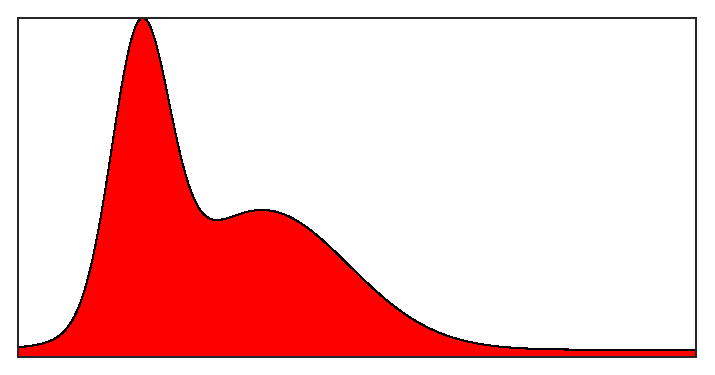
\includegraphics[width=0.95\linewidth]{figure/fig2.11/input-mu.eps}
		\caption*{$\alpha$}
	\end{minipage}
	\begin{minipage}{0.33\linewidth}
		\centering
		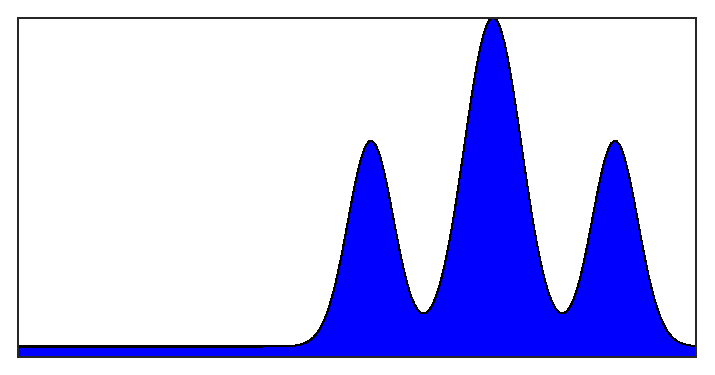
\includegraphics[width=0.95\linewidth]{figure/fig2.11/input-nu.eps}
		\caption*{$\beta$}
	\end{minipage}
	\begin{minipage}{0.33\linewidth}
		\centering
		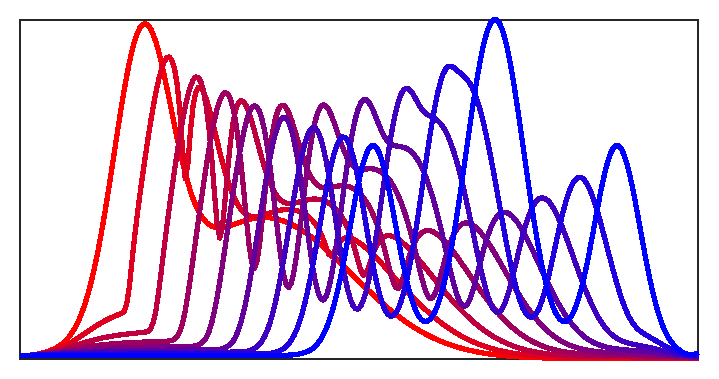
\includegraphics[width=0.95\linewidth]{figure/fig2.11/interp-bary.eps}
		\caption*{$(tT+(1-t)\text{Id})_\#\alpha$}
	\end{minipage}
	%\qquad
	\vspace{1em}
	
	\begin{minipage}{0.24\linewidth}
		\centering
		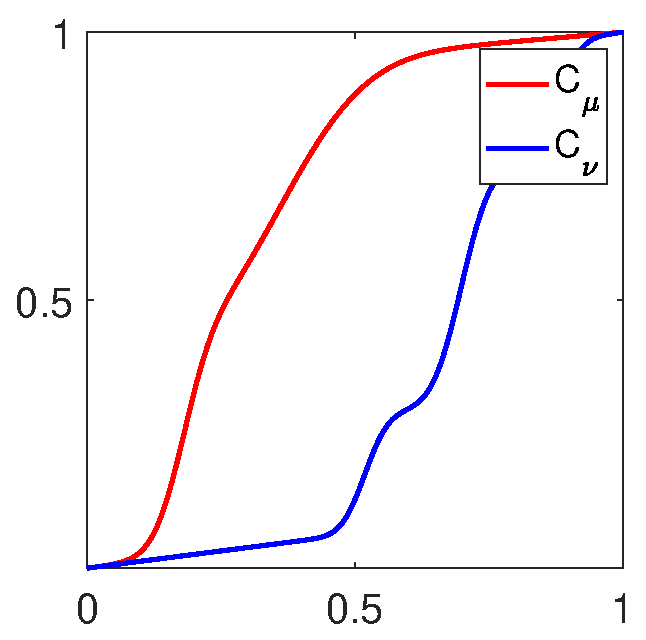
\includegraphics[width=0.95\linewidth]{figure/fig2.11/cumul.eps}
		\caption*{$(\mathcal{C}_\alpha,\mathcal{C}_\beta)$}
	\end{minipage}
	\begin{minipage}{0.24\linewidth}
		\centering
		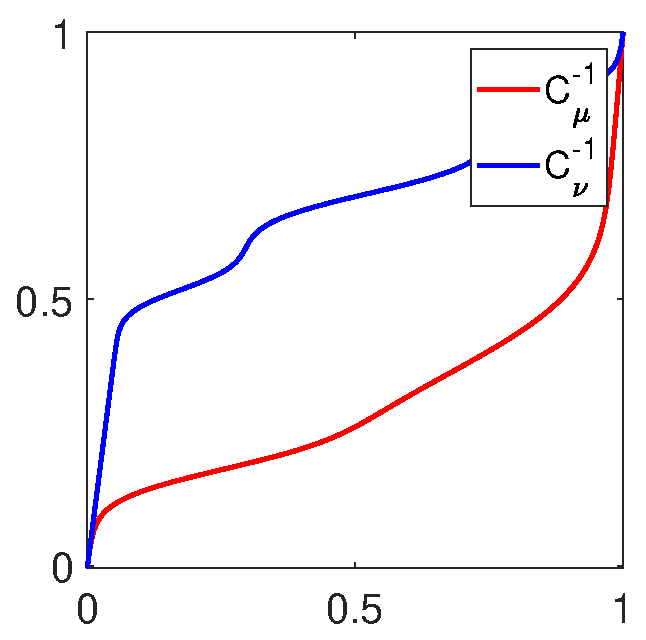
\includegraphics[width=0.95\linewidth]{figure/fig2.11/icumul.eps}
		\caption*{$(\mathcal{C}_\alpha^{-1},\mathcal{C}_\beta^{-1})$}
	\end{minipage}
	\begin{minipage}{0.24\linewidth}
		\centering
		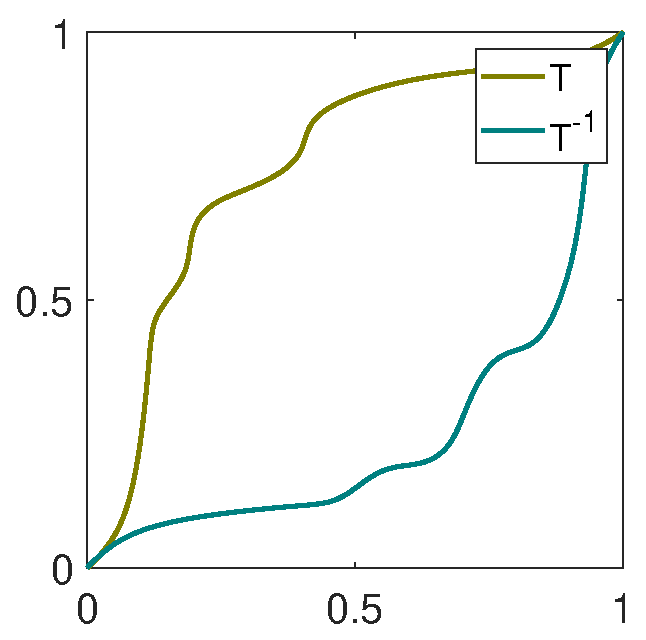
\includegraphics[width=0.95\linewidth]{figure/fig2.11/transports.eps}
		\caption*{$(T,T^{-1})$}
	\end{minipage}
	\begin{minipage}{0.24\linewidth}
		\centering
		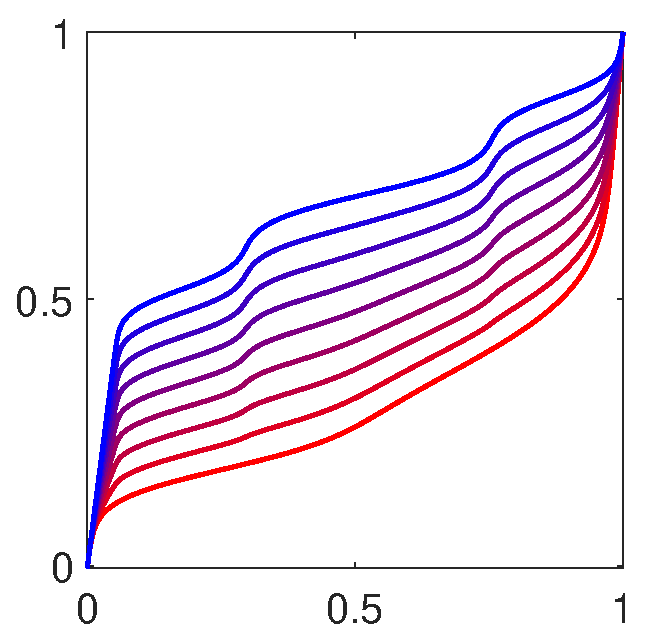
\includegraphics[width=0.95\linewidth]{figure/fig2.11/interp-cumul.eps}
		\caption*{$(1-t)\mathcal{C}_\alpha^{-1}+t\mathcal{C}_\beta^{-1}$}
	\end{minipage}
	
	\vspace{1em}
	\caption{一维最优传输及其位移插值的计算结果,借助累积函数按(2.19)式计算}
	\label{图2.11}
\end{figure}


\begin{postulate}[正态分布的距离]
设$\alpha=\mathcal{N}(\mathbf{m}_\alpha,\mathbf{\Sigma}_\alpha)$与$\beta=\mathcal{N}(\mathbf{m}_\beta,\mathbf{\Sigma}_\beta)$是$\mathbb{R}^d$上的两个正态分布,那么我们可以证明,下述映射
\begin{equation}
    \label{2.40}
    T:x\mapsto \mathbf{m}_\beta+A(x-\mathbf{m}_\alpha)
\end{equation}

其中
\begin{equation*}
    A=\mathbf{\Sigma}_\alpha^{-\frac{1}{2}}\left( \mathbf{\Sigma}_\alpha^{\frac{1}{2}} \mathbf{\Sigma}_\beta \mathbf{\Sigma}_\alpha^{\frac{1}{2}} \right)^{\frac{1}{2}} \mathbf{\Sigma}_\alpha^{-\frac{1}{2}} = A^T
\end{equation*}

满足$T_\#\rho_\alpha=\rho_\beta$。事实上,我们只需证明变量代换公式(2.8)成立即可。由于:
\begin{align*}
    \rho_\beta(T(x)) &= \text{det}(2\pi\mathbf{\Sigma}_\beta)^{-\frac{1}{2}}\exp{(-\langle T(x)-\mathbf{m}_\beta, \mathbf{\Sigma}_\beta^{-1}(T(x)-\mathbf{m}_\beta) \rangle)}\\
    &= \text{det}(2\pi\mathbf{\Sigma}_\beta)^{-\frac{1}{2}}\exp{(-\langle x-\mathbf{m}_\alpha, A^T\mathbf{\Sigma}_\beta^{-1} A(x-\mathbf{m}_\alpha) \rangle)}\\
    &= \text{det}(2\pi\mathbf{\Sigma}_\beta)^{-\frac{1}{2}}\exp{(-\langle x-\mathbf{m}_\alpha, \mathbf{\Sigma}_\alpha^{-1} (x-\mathbf{m}_\alpha) \rangle)}
\end{align*}

又由于$T$是线性映射,我们有:
\begin{equation*}
    |\det T'(x)| = \det A = \left(\frac{\det \mathbf{\Sigma}_\beta}{\det \mathbf{\Sigma}_\alpha}\right)^{\frac{1}{2}}
\end{equation*}

结合上述两式我们得到$\rho_\alpha(x) = |\det T'(x)|\rho_\beta(T(x))$,这意味着$T_\#\alpha=\beta$。不难注意到$T$是凸函数$\psi:x\mapsto \frac{1}{2}\langle x-\mathbf{m}_\alpha,A(x-\mathbf{m}_\alpha)\rangle + \langle \mathbf{m}_\beta, x\rangle$的梯度,根据Brenier定理[1991](见注记2.24),$T$就是最优传输解。映射$T$与对应的势$\psi$都在图2.12与图2.13中给出。

通过计算$\rho_\alpha$的一阶矩和二阶矩,我们得到:
\begin{equation}
    \label{2.41}
    \mathcal{W}_2^2(\alpha,\beta) = ||\mathbf{m}_\alpha,\mathbf{m}_\beta||^2 + \mathcal{B}(\mathbf{\Sigma}_\alpha,\mathbf{\Sigma}_\beta)^2
\end{equation}

其中$\mathcal{B}$就是正定矩阵之间所谓的Bures度量(也可见[Forrester and Kieburg, 2016]):
\begin{equation}
    \label{2.42}
    \mathcal{B}(\mathbf{\Sigma}_\alpha,\mathbf{\Sigma}_\beta)^2 \overset{\text{def}}{=} \text{tr} \left( \mathbf{\Sigma}_\alpha + \mathbf{\Sigma}_\beta - 2(\mathbf{\Sigma}_\alpha^{1/2}\mathbf{\Sigma}_\beta\mathbf{\Sigma}_\alpha^{1/2})^{1/2} \right)
\end{equation}

其中$\mathbf{\Sigma}^{1/2}$是矩阵的平方根。不难证明,$\mathcal{B}$定义了协方差矩阵之间的距离,并且$\mathcal{B}^2$关于它的两个自变量都是凸的。在$\mathbf{\Sigma}_\alpha=\text{diag}(r_i)_i$和$\mathbf{\Sigma}_\beta=\text{diag}(s_i)_i$的情形下,Bures度量就是Hellinger距离:
\begin{equation*}
    \mathcal{B}(\mathbf{\Sigma}_\alpha,\mathbf{\Sigma}_\beta)=||\sqrt{r}-\sqrt{s}||_2
\end{equation*}

对于一维正态分布,$\mathcal{W}_2$就是由正态分布的期望和标准差构成的二维平面$(\mathbf{m},\sqrt{\mathbf{\Sigma}})$上的欧式距离,如图2.14所示。对于正态分布的瓦瑟斯坦几何结构的详细研究,读者可以参见[Takatsu, 2011];对于Bures测度的进一步考虑,读者可以看最新研究[Malag\`o等人, 2018, Bhatia等人, 2018]。近期也有对Bures测度的应用研究,例如应用于单词的概率嵌入计算[Muzellec and Cuturi, 2018]、Kalman滤波的鲁棒扩展计算[Shafieezadeh Abadeh等人, 2018]、再生核希尔伯特空间中的协方差函数[Mallasto and Feragen, 2017]。
\end{postulate}

\begin{figure}[H]
    \centering
    \includegraphics[width=0.7\textwidth]{figure/fig2.12.png}
    \caption{两个正态分布$\rho_\alpha,\rho_\beta$,用密度函数的等高线图表示,其期望与协方差矩阵分别为$\mathbf{m}_\alpha=(-2,0),\mathbf{\Sigma}_\alpha=\frac{1}{2}\begin{pmatrix}1 & -\frac{1}{2}\\-\frac{1}{2} & 1\end{pmatrix}$与$\mathbf{m}_\beta=(3,1),\mathbf{\Sigma}_\beta=\begin{pmatrix}2 & \frac{1}{2}\\\frac{1}{2} & 1\end{pmatrix}$。箭头的起点是平面上随机取的点$x$,终点是其最优传输映射对应的像点$T(x)=\mathbf{m}_\beta+A(x-\mathbf{m}_\alpha)$}
    \label{图2.12}
\end{figure}

\begin{figure}[H]
    \centering
    \includegraphics[width=0.8\textwidth]{figure/fig2.13.png}
    \caption{和图2.12中一样的正态分布密度函数$\rho_\alpha, \rho_\beta$,用三维曲面图表示。上方的曲面是Brenier势$\psi$使得$T=\nabla \psi$(图中为了将两者图像分开显示,给了$\psi$的曲面一个$+50$的位移,另外为了视觉上更直观,将正态分布密度的值乘了$100$作图)}
    \label{图2.13}
\end{figure}

\begin{figure}[H]
	\centering
	\begin{minipage}{0.45\linewidth}
		\centering
		\includegraphics[width=0.8\linewidth]{figure/fig2.14/interp-density.eps}
	\end{minipage}
	\begin{minipage}{0.45\linewidth}
		\centering
		\includegraphics[width=0.8\linewidth]{figure/fig2.14/plane.eps}
	\end{minipage}
	%\qquad
	\vspace{1em}
	\caption{左图:一维正态分布的位移插值计算结果,记$\mathcal{G}_{m,\sigma}(x)\overset{\text{def}}{=}\frac{1}{\sqrt{2\pi}\sigma}e^{-\frac{(x-m)^2}{2\sigma^2}}$为正态分布密度函数,则位移插值可表示为$\mathcal{G}_{(1-t)m_0+tm_1,(1-t)\sigma_0+t\sigma_1}$。右图(译者加):位移插值分布的期望、标准差在$(m,\sigma)$平面上的位置,点的颜色与左图图像的颜色相对应。}
	\label{图2.14}
\end{figure}

\begin{postulate}[椭球等高分布的距离]
Gelbrich给出了比注记2.31中更一般的结果:将正态分布的Bures测度推广到更一般的椭球等高分布上。简言之,我们可以首先证明:当两个概率测度的期望和协方差矩阵确定时,他们的瓦瑟斯坦距离在二者都为正态分布时取得下界[Gelbrich, 1990, Theorem 2.1]。此外,可以将闭形式(2.41)推广到椭球等高分布族上:若两个密度函数$\rho_\alpha,\rho_\beta$属于这样的一个族,即$\rho_\alpha,\rho_\beta$可以用期望和正定参数在任意位置$x$中表示:
\begin{align*}
    \rho_\alpha(x)&=\frac{1}{\sqrt{\det(\mathbf{A})}}h(\langle x-\mathbf{m}_\alpha, \mathbf{A}^{-1}(x-\mathbf{m}_\alpha) \rangle)\\
    \rho_\beta(x)&=\frac{1}{\sqrt{\det(\mathbf{B})}}h(\langle x-\mathbf{m}_\beta, \mathbf{B}^{-1}(x-\mathbf{m}_\beta) \rangle)
\end{align*}

其中$h$是某个非负值函数,满足如下积分式:
\begin{equation*}
    \int_{\mathbb{R}^d} h(\langle x,x \rangle) \text{d}x = 1
\end{equation*}

则它们的最优传输映射也是(2.40)中的线性映射,且瓦瑟斯坦距离也由(2.41)给出,稍有不同的是Bures测度将会乘一个依赖于生成函数$h$的系数。例如,对于正态分布$h(t)=e^{-t/2}$,系数为$1$;对于椭球体上的均匀分布($h$是$[0,1]$上的示性函数),系数为$1/(d+2)$。这个结果可以由下述事实得到:椭球分布的协方差矩阵是其正定参数乘上一个常数[G\'omez等人, 2003, Theo. 4(ii)],且椭球分布的瓦瑟斯坦距离是关于他们的协方差矩阵之间的Bures距离的一个函数[Gelbrich, 1990, Cor. 2.5]。
\end{postulate}

\chapter{算法基础\footnote{译者注:本章中,原文的\S 3.6为“对偶上升法”(Dual Ascent Method),译者认为该小节很无趣,其思想与\S 3.5重复,且不如最小费用最大流的建模精妙,应用价值也不高,故不译。此外,译者也推荐使用最小费用最大流建模来解决最优传输问题,原书中没有提及,感兴趣的读者可以参考OI/ACM的相关资料,当然这个方法复杂度较高,不适用于大规模问题,对于大规模问题还是推荐第四章的Sinkhorn算法。}}

本章介绍求解离散最优传输或其对偶问题的常见算法,包括源自组合优化的算法和线性规划。

这些算法的起源可追溯至二战期间,在此之前有Tolston的开创新工作[1930],在战争期间,Hitchcock[1941]和Kantorovich[1942]将最优资源调度问题一般化,并用形式化语言表述。所有这些工作,包括后来Koopmans[1949]所作的研究,都没有给出可证明正确性的求解算法(循环破坏法\footnote{译者注:原文为cycle violation method}已经被Tolston[1939]证明为启发式算法)。一直等到随着单纯形法的出现,线性规划领域彻底成熟,这时才能严格地求解最优传输。

最优传输问题可以转化为求解一个线性规划,其目标函数为线性函数,约束条件是关于某些变量的线性等式或不等式。我们也能发现,最优传输问题在线性规划中是相当特殊的一类。首先,Dantzig早期研究线性规划求解的动机,很大程度上是为了求解传输问题[Dantzig, 1949, p. 210]。其次,尽管最优传输只是线性规划的一个特例,它却仍是优化领域的焦点。这是因为,线性规划中有一类相当重要的问题——最小费用网络流[Korte and Vygen, 2012, p.213, Lem. 9.3],而得益于Ford与Fulkerson[1962]的工作,人们发现最优传输与其息息相关(事实上二者甚至是等价的)。总之,自从数学规划诞生[Dantzig, 1951]以来,最优传输就一直是备受关注的课题。作为一个优化问题的例子,它至今仍广泛用于优化的科普[Nocedal and Wright, 1991, \S 1, p. 4]。

\section{康托洛维奇问题的线性规划解法}

回顾原始的最优传输问题(2.11):
\begin{equation}
    \label{3.1}
    L_\mathbf{C}(\mathbf{a,b})=\min\limits_{\mathbf{P}\in\mathbf{U(a,b)}} \sum_{i,j} \mathbf{C}_{i,j}\mathbf{P}_{i,j}
\end{equation}

下面我们考虑将上述问题表述为线性规划的标准形式,即:线性形式的目标函数、矩阵-向量乘积形式的等式约束、变量的非负约束。设$\mathbb{I}_n$为$n$阶单位矩阵,$\otimes$表示Kronecher乘积\footnote{译者注:对矩阵$A=(a_{ij})\in\mathbb{R}^{n\times m},B=(b_{ij})\in\mathbb{R}^{pq}$,其结果是一个$np\times mq$的矩阵:$A\otimes B=\begin{bmatrix} a_{11}B & a_{12}B & \cdots & a_{1n}B\\ a_{21}B & a_{22}B & \cdots & a_{2n}B \\ \vdots & \vdots & \ddots & \vdots \\ a_{n1}B & a_{n2}B & \cdots & a_{nn}B\end{bmatrix}$}。下述$(n+m)\times nm$的矩阵:
\begin{equation*}
    \mathbf{A}=\begin{bmatrix} \mathbbm{1}_n^T\otimes \mathbb{I}_m\\ \mathbb{I}_n\otimes \mathbbm{1}_m^T\end{bmatrix}\in\mathbb{R}^{(n+m)\times nm}
\end{equation*}

可以用来表示$\mathbf{P}$在$\mathbf{U(a,b)}$中应当满足的行和约束与列和约束。首先将$\mathbf{P}\in\mathbb{R}^{n\times m}$拍扁成一个向量$\mathbf{p}\in\mathbb{R}^{nm}$,其第$i+n(j-1)$个分量为$\mathbf{P}_{ij}$(即对$\mathbf{P}$按列扫描),得到如下等价表述:
\begin{equation*}
    \mathbf{P}\in\mathbb{R}^{n\times m}\in\mathbf{U(a,b)} \Longleftrightarrow \mathbf{p}\in\mathbb{R}^{nm}_+,\mathbf{Ap}=\begin{bmatrix}\mathbf{a}\\ \mathbf{b}\end{bmatrix}
\end{equation*}

因此我们可以将原始的最优传输问题写为:
\begin{align}
    \label{3.2}
     L_\mathbf{C}(\mathbf{a,b})= &\min \quad \mathbf{c}^T\mathbf{p}\\
     &\text{s.t.} \quad \mathbf{p}\in\mathbb{R}_+^{nm} \nonumber \\ 
     & \quad \quad \mathbf{Ap}=\begin{bmatrix}\mathbf{a}\\ \mathbf{b}\end{bmatrix} \nonumber
\end{align}

其中$nm$维向量$\mathbf{c}$是由费用矩阵$\mathbf{C}$按列扫描得到的。

\begin{postulate}
注意到上述$n+m$条约束中有一条是冗余的,换言之,矩阵$A$的行向量不是线性无关的。事实上,将$A$的前$n$行相加,与后$m$列相加,得到的结果是一样的(即:$[\mathbbm{1}_n\;\;\mathbb{0}_m]A=[\mathbb{0}_n\;\;\mathbbm{1}_m]A=\mathbbm{1}_{nm}^T$)\footnote{译者注:原文为$A\begin{bmatrix}\mathbbm{1}_n\\ \mathbb{0}_m\end{bmatrix}=A\begin{bmatrix}\mathbb{0}_n\\ \mathbbm{1}_m\end{bmatrix}=\mathbbm{1}_{nm}^T$,译者认为有误,故作修改。}。可以证明,删除$A$的某一行以及$[\mathbf{a}^T\;\;\mathbf{b}^T]^T$中对应分量,能得到一个适定的线性系统。出于简洁性考虑,以及为了避免处理$\mathbf{a}$和$\mathbf{b}$时的不对称,我们保留具有冗余约束的形式,也请记住在我们的计算过程中可能会突然出现退化情况。
\end{postulate}

根据线性规划的对偶化[Bertsimas and Tsitsiklis, 1997, p.143],(3.2)的对偶问题定义为:
\begin{align}
    \label{3.3}
     L_\mathbf{C}(\mathbf{a,b})= &\max \quad \begin{bmatrix}\mathbf{a}\\ \mathbf{b}\end{bmatrix}^T\mathbf{h}\\
     &\text{s.t.} \quad \mathbf{h}\in\mathbb{R}^{n+m} \nonumber \\ 
     & \quad \quad \mathbf{A}^T\mathbf{h}\leq \mathbf{c} \nonumber
\end{align}

注意到这个规划和问题(2.20)\footnote{译者注:原文指向(2.4),译者认为有误,应当指向(2.20)}是等价的。

\begin{postulate}
我们给出上述对偶结果的一个简单推导,它可以被看做注记2.21中所作讨论的一个直接公式。强对偶性,即(3.2)与(3.3)最优值相同,需要很长的证明[Bertsimas and Tsitsiklis, 1997, \S 4.10]。为了简化符号,我们记$\mathbf{q}=\begin{bmatrix}\mathbf{a}\\ \mathbf{b}\end{bmatrix}$。考虑将原始的最优传输问题松弛化,我们对约束$\mathbf{Ap=q}$不再作强制要求,而是将其作为惩罚项$\mathbf{h}^T\mathbf{Ap-q}$引入,其中$\mathbf{h}\in\mathbb{R}^{n+m}$是一个任意向量。则松弛化后的问题,其最优值直接取决于代价向量$\mathbf{h}$,可以写为:
\begin{equation*}
    H(\mathbf{h})\overset{\text{def}}{=} \min\limits_{\mathbf{p}\in\mathbb{R}^{nm}_+} \; \mathbf{c}^T\mathbf{p}-\mathbf{h}^T(\mathbf{Ap-q})
\end{equation*}

首先注意到上述松弛化问题没有对$\mathbf{p}$的边值约束。由于上述最小化问题允许了更多可行解$\mathbf{p}$,我们可以期望$H(\mathbf{h})$不会超过$\bar z=L_\mathbf{C}(\mathbf{a,b})$。事实上,设$\mathbf{p}^\star$是原始问题(3.1)的任意一个最优解,我们有:
\begin{equation*}
    \min\limits_{\mathbf{p}\in\mathbb{R}^{nm}_+} \; \mathbf{c}^T\mathbf{p}-\mathbf{h}^T(\mathbf{Ap-q}) \leq \mathbf{c}^T\mathbf{p}^\star-\mathbf{h}^T(\mathbf{Ap}^\star-\mathbf{q})=\mathbf{c}^T\mathbf{p}^\star=\bar z
\end{equation*}

因此,对任何代价向量$\mathbf{h}$,上述方法定义的问题能用于计算原始问题(3.1)的最优上界。这个函数被称为$L$的拉格朗日对偶函数。对偶理论的目的是通过取遍所有代价向量$\mathbf{h}$来最大化$H$,以计算出$\underline{z}$的最优下界,即:
\begin{equation*}
    \underline{z}=\max\limits_{\mathbf{h}} \left( H(\mathbf{h})=\max\limits_{\mathbf{h}}\mathbf{h}^T\mathbf{q} + \min\limits_{\mathbf{p}\in\mathbb{R}^{nm}_+}(\mathbf{c}-\mathbf{A}^T\mathbf{h})^T\mathbf{p} \right)
\end{equation*}

对于上式中第二项引入的关于$\mathbf{p}$的最小化,不难验证,若$\mathbf{c}^T-\mathbf{A}^T\mathbf{h}$存在一个负分量,则这个最小化值为$-\infty$。事实上,若对某给定的$i\leq n+m$,有$\mathbf{c}^T_i-(\mathbf{A}^T\mathbf{h})_i<0$,那么只需取$\mathbf{p}$为标准基向量$\mathbf{e}_i$乘上一个任意大的正值,就能得到无界的结果。因此当试图最大化$H(\mathbf{h})$的下界时,我们应当限制$\mathbf{h}$满足$\mathbf{A}^T\mathbf{h}\leq \mathbf{c}$,在这个情况下可能的最大下界就是:
\begin{equation*}
    \underline{z}=\max\limits_{\begin{array}{c}\mathbf{h}\in\mathbb{R}^{n+m}\\ \mathbf{A}^T\mathbf{h}\leq \mathbf{c}\end{array}}\; \mathbf{h}^T\mathbf{q}
\end{equation*}

由此我们得到弱对偶性结果,即$\underline{z}\leq \bar{z}$。
\end{postulate}

\section{$c$变换}

在这一节中,我们给出最优传输对偶问题(3.3)的一个重要性质,它在\S 5.1中的半离散最优传输中有着更重要的意义。这一节依赖于原始公式(2.20),其根据行和约束与列和约束分离对偶变量:
\begin{equation}
    \label{3.4}
    L_\mathbf{C}(\mathbf{a,b})=\max\limits_{(\mathbf{f,g})\in\mathbf{R}(\mathbf{C})} \langle \mathbf{f,a}\rangle + \langle \mathbf{g,b} \rangle
\end{equation}

考虑可行对偶对$(\mathbf{f,g})$,若固定$\mathbf{f}$,则$\mathbf{g}$显然取$\mathbf{f^C}\in\mathbb{R}^m$时目标函数达到最优,其中$\mathbf{f^C}$定义为:
\begin{equation*}
    (\mathbf{f^C})_j=\min\limits_{i\in\mathbb{[}n\mathbb{]}}\mathbf{C}_{ij}-\mathbf{f}_i
\end{equation*}

称为$\mathbf{f}$的$c$变换。事实上不难证明$(\mathbf{f,f^C})\in\mathbf{R(C)}$,且$\mathbf{f^C}$是可能使此约束成立的最大向量。因此我们有:
\begin{equation*}
    \langle \mathbf{f,a}\rangle + \langle \mathbf{g,b} \rangle \leq \langle \mathbf{f,a}\rangle + \langle \mathbf{f^C,b} \rangle
\end{equation*}

借助这个结果,我们可以将最大化问题重述为仅仅关于$\mathbf{f}$的形式:
\begin{equation}
    \label{3.5}
    L_\mathbf{C}(\mathbf{a,b})=\max\limits_{(\mathbf{f})\in\mathbb{R}^n} \langle \mathbf{f,a}\rangle + \langle \mathbf{f^C,b} \rangle
\end{equation}

同理,我们也可以先固定$\mathbf{g}$,然后考虑$\mathbf{g}$的$\bar c$变换,即:
\begin{equation*}
    (\mathbf{g^{\bar C}})_i=\min\limits_{j\in\mathbb{[}m\mathbb{]}}\mathbf{C}_{ij}-\mathbf{g}_j\in\mathbb{R}^n
\end{equation*}

类似地,也满足:
\begin{equation*}
    \langle \mathbf{f,a}\rangle + \langle \mathbf{g,b} \rangle \leq \langle \mathbf{g^{\bar C},a}\rangle + \langle \mathbf{g,b} \rangle
\end{equation*}

若给定初始的$\mathbf{f}$,我们可以取$\mathbf{g}$为$\mathbf{f}$的$c$变换,然后重新取$\mathbf{f}$为$\mathbf{g}$的$\bar c$变换,如此交替迭代下去,我们就有:
\begin{equation*}
    \langle \mathbf{f,a}\rangle + \langle \mathbf{f^C,b} \rangle \leq \langle \mathbf{f^{C\bar C},a}\rangle + \langle \mathbf{f^C,b} \rangle \leq \langle \mathbf{f^{C \bar C},a}\rangle + \langle \mathbf{f^{C \bar{C} C},b} \rangle \leq \cdots
\end{equation*}

我们希望这样的序列能一直递增下去,这样就可能最终收敛于最大值。然而,这是行不通的,因为交替进行$c$变换与$\bar c$变换,会很快进入到一个稳定点。

\begin{proposition}[$c$变换与$\bar c$变换的基本性质]
我们先约定,下述向量之间的等式与不等式都是指二者所有对应元素之间均满足的关系。对于$c$变换与$\bar c$变换,我们有:

\begin{enumerate}
    \item $\mathbf{f}\leq \mathbf{f}' \Rightarrow \mathbf{f^C}\geq \mathbf{f}'^{\mathbf{C}}$
    \item $\mathbf{f^{C\bar C}}\geq \mathbf{f},\; \mathbf{g}^{\bar{\mathbf{C}}\mathbf{C}}\geq \mathbf{g}$
    \item $\mathbf{f^{C\bar{C}C}}=\mathbf{f^C}$
\end{enumerate}
\end{proposition}

\begin{proof}
第一个不等式由$c$变换的定义易得。现展开$\mathbf{f^{C\bar C}}$的定义,我们有:
\begin{equation*}
    \left(\mathbf{f^{C\bar C}}\right)_i = \min\limits_{j\in\mathbb{[}m\mathbb{]}} \left(\mathbf{C}_{ij}-\mathbf{f^C}_j\right) = \min\limits_{j\in\mathbb{[}m\mathbb{]}}\left( \mathbf{C}_{ij}- \min\limits_{i'\in\mathbb{[}n\mathbb{]}}\left(\mathbf{C}_{i'j}-\mathbf{f}_{i'}\right) \right)
\end{equation*}

注意到$- \min\limits_{i'\in\mathbb{[}n\mathbb{]}}\left(\mathbf{C}_{i'j}-\mathbf{f}_{i'}\right)\geq - \left(\mathbf{C}_{ij}-\mathbf{f}_{i}\right)$,因此我们有:
\begin{equation*}
    \left(\mathbf{f^{C\bar C}}\right)_i \geq \min\limits_{j\in\mathbb{[}m\mathbb{]}} \mathbf{C}_{ij}-\mathbf{C}_{ij}+\mathbf{f}_i = \mathbf{f}_i
\end{equation*}

同理可得$\mathbf{g}^{\bar{\mathbf{C}}\mathbf{C}}\geq \mathbf{g}$。现令$\mathbf{g}=\mathbf{f^C}$,则$\mathbf{g^{\bar C}}=\mathbf{f^{C \bar C}}\geq \mathbf{f}$,于是由1,有$\mathbf{f^{C\bar{C}C}}\leq \mathbf{f^C}$,然而由2中$\mathbf{g}$的不等式,又有$\mathbf{f^{C\bar{C}C}}\geq \mathbf{f^C}$,因此3中的等式得证。证毕。
\end{proof}

\section{互补松弛}

原始问题(3.2)与对偶问题(3.3),(2.20)都可以独立地求解以得到最优耦合子$\mathbf{P}^\star$和最优对偶对$(\mathbf{f}^\star,\mathbf{g}^\star)$。下面这条命题给出了它们的关系。

\begin{proposition}
令$\mathbf{P}^\star$和$(\mathbf{f}^\star,\mathbf{g}^\star)$分别为原始问题(2.11)与对偶问题(2.20)的最优解。则对任意$(i,j)\in\mathbb{[}n\mathbb{]}\times \mathbb{[}m\mathbb{]}$,有$\mathbf{P}^\star_{ij}\left(\mathbf{C}_{ij}-\left( \mathbf{f}_i^\star + \mathbf{g}_j^\star \right)\right)=0$。换言之,若$\mathbf{P}_{ij}^\star>0$,则必有$\mathbf{f}_i^\star+\mathbf{g}_j^\star = \mathbf{C}_{ij}$;若$\mathbf{f}_i^\star+\mathbf{g}_j^\star < \mathbf{C}_{ij}$,则必有$\mathbf{P}_{ij}^\star=0$。
\end{proposition}

\begin{proof}
根据强对偶性,我们有$\langle \mathbb{P}^\star,\mathbb{C}\rangle = \langle \mathbb{f}^\star,\mathbb{a}\rangle + \langle \mathbb{g}^\star,\mathbb{b} \rangle$。注意到有行和与列和约束:$\mathbf{P}^\star\mathbbm{1}_m=\mathbb{a}$与$\mathbf{P}^{\star T}\mathbbm{1}_n=\mathbb{b}$。因此:
\begin{align*}
    \langle \mathbf{f}^\star,\mathbf{a}\rangle + \langle \mathbf{g}^\star,\mathbf{b} \rangle &= \langle \mathbf{f}^\star,\mathbf{P}^\star\mathbbm{1}_m\rangle + \langle \mathbf{g}^\star,\mathbf{P}^{\star T}\mathbbm{1}_n \rangle \\
    &= \langle \mathbf{f}^\star\mathbbm{1}_m^T,\mathbf{P}^\star \rangle + \langle \mathbbm{1}_n\mathbf{g}^{\star T},\mathbf{P}^{\star} \rangle
\end{align*}

由上述结果可得:
\begin{equation*}
    \langle \mathbf{P}^\star, \mathbf{C}-\mathbf{f}^\star \oplus \mathbf{g}^\star \rangle = 0
\end{equation*}

由于$(\mathbf{f}^\star, \mathbf{g}^\star)$属于对偶约束(2.21)的多面体集,故矩阵$\mathbf{C}-\mathbf{f}^\star \oplus \mathbf{g}^\star$的每个元素都必须是非负的。因此,由于$\mathbf{P}^\star$的每个元素都是非负的,上面导出的内积为0的约束必然使得:当$\mathbf{P}_{ij}^\star>0$,$\mathbf{C}_{ij}-(\mathbf{f}_i^\star+\mathbf{g}_j^\star)$必为零;当$\mathbf{C}_{ij}>\mathbf{f}_i^\star+\mathbf{g}_j^\star$,$\mathbf{P}_{ij}^\star$必为零。证毕。
\end{proof}

\vspace{1.5em}

这个结果反之也是成立的。首先我们定义原始问题变量和对偶问题变量的互补。

\begin{definition}[互补]
称矩阵$\mathbf{P}\in\mathbb{R}^{n\times m}$和向量对$(\mathbf{f,g})$关于$\mathbf{C}$互补,若对任意满足$\mathbf{P}_{ij}>0$的下标$(i,j)$,总有$\mathbf{C}_{ij}=\mathbf{f}_i+\mathbf{g}_j$。
\end{definition}

若原始问题与对偶问题的一对可行解恰好互补,则我们可以推知它们是最优解,如下。

\begin{proposition}
若矩阵$\mathbf{P}$和向量对$(\mathbf{f,g})$分别是原始问题(2.11)与对偶问题(2.20)的可行解,且关于$\mathbf{C}$互补,则它们分别是原始问题和对偶问题的最优解。
\end{proposition}

\begin{proof}
根据弱对偶性,我们有:
\begin{equation*}
    L_\mathbf{C}(\mathbf{a,b})\leq \langle \mathbf{P},\mathbf{C} \rangle = \langle \mathbf{P}, \mathbf{f}\oplus \mathbf{g} \rangle = \langle \mathbf{a,f} \rangle + \langle \mathbf{b,g} \rangle \leq L_\mathbf{C}(\mathbf{a,b})
\end{equation*}

因此$\mathbf{P}$和$(\mathbf{f,g})$分别是原始问题和对偶问题的最优解。证毕。
\end{proof}

\section{传输方案的可行极值解}

凸集的顶点或极值点是指满足下述条件的点$\mathbf{x}$:若集合中存在$\mathbf{y,z}$使得$\mathbf{x}=(\mathbf{y}+\mathbf{z})/2$,则必有$\mathbf{x=y=z}$。一个可行集非空且有界的线性规划问题,其最优点必然落在可行集的顶点(称可行集顶点为“可行极值解”)处[Bertsimas and Tsitsiklis, 1997, p.65, Theo. 2.7]。由于原始最优传输问题(3.2)的可行集$\mathbf{U(a,b)}$是有界的,我们可以将最优解$\mathbf{P}$的范围缩小到多面体集$\mathbf{U(a,b)}$的极值点上。$\mathbf{U(a,b)}$的极值点$\mathbf{P}$具有非常有趣的结构,是一个被广泛研究的课题[Brualdi, 2006, \S 8]。这个结构需要借助二分图的形式来表述最优传输问题。

\subsection{可行极值解支点的树形结构}

令$V=(1,2,...,n)$与$V'=(1',2',...,m')$为两个点集。我们为$V'$中的点加一撇,以示与$V$中的点区分。考虑点集$V\cup V'$,有$n+m$个点,其所有的有向边集为$\mathcal{E}=\{(i,j'):i\in\mathbb{[}n\mathbb{]},j\in\mathbb{[}m\mathbb{]}\}$(这里$j'$表示$V'$中的$j$号点)。对于每一条边$(i,j')$,我们有对应的费用$\mathbf{C}_{ij}$。$V$与$V'$构成的完全二分图即为$\mathcal{G}=(V\cup V',\mathcal{E})$。一个传输方案就是图中的一个网络流,满足:源点为$V$中的点,点$i$流出的流量即为$\mathbf{a}_i$;汇点为$V'$中的点,点$j'$流入的流量即为$\mathbf{b}_j$。如图3.1所示。$\mathbf{U(a,b)}$中的可行极值解具有如下性质。

\begin{figure}[H]
    \centering
    \includegraphics[width=0.8\textwidth]{figure/fig3.1.png}
    \caption{最优传输问题转化为二分图网络流问题。这里$n=3,m=4$。源直方图$\mathbf{a}$的所有分量都作为源点在左侧以$1,2,3$标注;目标直方图$\mathbf{b}$的所有分量都作为汇点在右侧以$1',2',3',4'$标注。此图显然是二分图,源点与汇点一一连接,没有额外的边。每条边$(i,j')$都有对应的费用$\mathbf{C}_{ij}$。一个可行流如右图所示。由命题3.4可知,右图的例子不是可行极值解,因为它是有环的。}
    \label{图3.1}
\end{figure}

\begin{proposition}[可行极值解的树形结构]
令$\mathbf{P}$是$\mathbf{U(a,b)}$中的可行极值解。令$S(\mathbf{P})\subset \mathcal{E}$为非退化边集$\{ (i,j'):i\in\mathbb{[}n\mathbb{]},j\in\mathbb{[}m\mathbb{]},\mathbf{P}_{ij}>0 \}$。则图$G(\mathbf{P})\overset{\text{def}}{=}(V\cup V',S(\mathbf{P}))$是无环的。换言之,$\mathbf{P}$的非零元素不超过$n+m-1$个。
\end{proposition}

\begin{proof}
我们用反证法证明。设$\mathbf{P}$是$\mathbf{U(a,b)}$中的可行极值解,其非退化边集为$S(\mathbf{P})$,简记为$F$。现设$G=(V\cup V',F)$有环,即存在$k>1$,以及不重复的下标$i_1,...,i_{k}\in\mathbb{[}n\mathbb{]}$与$j_1,...,j_{k}\in\mathbb{[}m\mathbb{]}$,使得下述边集$H$是$F$的一个子集。
\begin{equation*}
    H=\{ (i_1,j_1'),(i_2,j_1'),(i_2,j_2'),...,(i_k,j_k'),(i_1,j_k')\}
\end{equation*}

现在来构造两个可行解矩阵$\mathbf{Q,R}$,使得$\mathbf{P}=(\mathbf{Q+R})/2$。考虑一个对应于$H$的有向环$\bar H$,即序列$i_1\to j_1',j_1'\to i_2,i_2\to j_2',...,i_k\to j_k',j_k'\to i_1$。取小流量$\varepsilon<\min_{(i,j')\in F}\mathbf{P}_{ij}$。考虑一个小扰动矩阵,其$(i,j)$元素为$\varepsilon$若$i\to j'\in\bar H$;为$-\varepsilon$若$j'\to i\in\bar H$\footnote{译者注:原书为$j\to i'\in\bar H$,译者认为有误。};其它情况为$0$。设矩阵$\mathbf{Q}=\mathbf{P+E}$,$\mathbf{R}=\mathbf{P-E}$,如图3.2所示。由于$\varepsilon$充分小,$\mathbf{Q,R}$中所有元素都是非负的。根据上述构造,$\mathbf{E}$的第$i_1,...,i_k$行中,每一行恰有一个元素为$\varepsilon$和一个元素为$-\varepsilon$,其余行全零(对$j_1,...,j_k$列同理)。因此有$\mathbf{E}\mathbbm{1}_m=\mathbb{0}_n$以及$\mathbf{E}^T\mathbbm{1}_n=\mathbb{0}_m$,因此$\mathbf{Q,R}$满足和$\mathbf{P}$一样的行和、列和约束,因此都是可行解。

这样我们就得到了$\mathbf{P}=(\mathbf{Q+R})/2$,其中$\mathbf{Q,R}\neq \mathbf{P}$且均为可行解。这与$\mathbf{P}$是可行极值解相矛盾。因此$S(\mathbf{P})$必然是无环的,从而不超过$n+m-1$条边,即$\mathbf{P}$的非零元素不超过$n+m-1$个。证毕。
\end{proof}

\begin{figure}[H]
    \centering
    \includegraphics[width=0.8\textwidth]{figure/fig3.2.png}
    \caption{对于一个非退化边集包含一个环的可行解$\mathbf{P}$,可以加以小扰动将其分解为两个可行解$Q,R$,使得$\mathbf{P}=(\mathbf{Q+R})/2$,从而否定了$\mathbf{P}$是可行极值解。}
    \label{图3.2}
\end{figure}

\subsection{左上角法}

左上角法(North-West Corner Rule, NW)是一种在$n+m$步操作内得到$\mathbf{U(a,b)}$中一个可行极值解的启发式方法。这个启发式方法可以用于初始化一个需要初值的算法,例如下一节将会提到的网络单纯形法。

左上角法首先需要给定$\mathbf{P}_{1,1}$的最大可能值,取为$\min(\mathbf{a}_1,\mathbf{b}_1)$。对于每一步操作,取$\mathbf{P}_{ij}$的值使得第$i$行的行和约束饱和,或使第$j$列的列和约束饱和,或在允许的情况下使它们同时饱和。然后更新下标$i,j$:若进行了行和饱和操作,则令$i$加一,$j$不变;若进行了列和饱和操作,则令$j$加一,$i$不变;若二者恰好同时能进行,则$i,j$均加一。上述过程直到$\mathbf{P}_{n,m}$取得值时终止。

形式化地,我们将算法表示如下:

\begin{algorithm}[]  %其中这里面不能有H不然会报错, 不过不影响结果
	\caption{North-West Corner Rule}%算法名字
	\KwIn{$\mathbf{a,b}$}%输入参数
	\KwOut{$\mathbf{P}$}%输出
	\Set $\mathbf{P}_{1,1}=\min(\mathbf{a}_1,\mathbf{b}_1)$
	
	\Set $r\gets \mathbf{a}_1,\;c\gets \mathbf{b}_1$
	
	\While{$i\leq n$ and $j\leq m$}{
	    \Set $t\gets \min(r,c)$
	    
	    \Set $\mathbf{P}_{i,j}\gets t$
	    
	    \Set $r\gets r-t,\; c\gets c-t$
	    
	    \If{r=0}{
	        \Set $i\gets i+1,\;r\gets \mathbf{a}_i$(if $i\leq n$)
	    }
	    
	    \If{c=0}{
	        \Set $j\gets j+1\;c\gets \mathbf{b}_j$(if $j\leq m$)
	    }
	}
\end{algorithm}

下面给出一个算例,其中$\mathbf{a}=[0.2,0.5,0.3]$以及$\mathbf{b}=[0.5,0.1,0.4]$:
\begin{equation*}
    \begin{bmatrix}
        \bullet & 0 & 0 \\
        0 & 0 & 0 \\
        0 & 0 & 0
    \end{bmatrix} \to 
    \begin{bmatrix}
        0.2 & 0 & 0 \\
        \bullet & 0 & 0 \\
        0 & 0 & 0
    \end{bmatrix} \to
    \begin{bmatrix}
        0.2 & 0 & 0 \\
        0.3 & \bullet & 0 \\
        0 & 0 & 0
    \end{bmatrix} \to
    \begin{bmatrix}
        0.2 & 0 & 0 \\
        0.3 & 0.1 & \bullet \\
        0 & 0 & 0
    \end{bmatrix} \to
        \begin{bmatrix}
        0.2 & 0 & 0 \\
        0.3 & 0.1 & 0.1 \\
        0 & 0 & \bullet
    \end{bmatrix} \to
    \begin{bmatrix}
        0.2 & 0 & 0 \\
        0.3 & 0.1 & 0.1 \\
        0 & 0 & 0.3
    \end{bmatrix}
\end{equation*}

我们记$\mathbf{NW(a,b)}$为左上角法得到的可行解。

注意到我们可以通过对$\mathbf{a,b}$的坐标事先作一个置换,然后用左上角法计算,将结果再置换回原顺序,这样就能得到更多的可行解。例如取置换$\sigma=(3,1,2)$与$\sigma'=(3,2,1)$,则$\mathbf{a}_\sigma=[0.3,0.2,0.5], \mathbf{b}_{\sigma'}=[0.4,0.1,0.5]$,以及$\sigma^{-1}=(2,3,1),\sigma'^{-1}=(3,2,1)$。可以观察到:
\begin{align*}
    \mathbf{NW}(\mathbf{a}_\sigma,\mathbf{b}_{\sigma'}) = \begin{bmatrix}
        0.3 & 0 & 0 \\
        0.1 & 0.1 & 0 \\
        0 & 0 & 0.5
    \end{bmatrix} \in \mathbf{U}(\mathbf{a}_\sigma,\mathbf{b}_{\sigma'})\\
    \mathbf{NW}_{\sigma^{-1},\sigma'^{-1} }(\mathbf{a}_\sigma,\mathbf{b}_{\sigma'}) = \begin{bmatrix}
        0 & 0.1 & 0.1 \\
        0.5 & 0 & 0 \\
        0 & 0 & 0.3
    \end{bmatrix} \in \mathbf{U}(\mathbf{a},\mathbf{b})
\end{align*}

令$\mathcal{N}(\mathbf{a,b})$为左上角法按这种方式能产生的所有可行解(称:左上角解):
\begin{equation*}
    \mathcal{N}(\mathbf{a,b})\overset{\text{def}}{=}\left\{ \mathbf{NW}_{\sigma^{-1},\sigma'^{-1}}(r_\sigma,c_{\sigma'}), \sigma,\sigma'\in S_d \right\}
\end{equation*}

显然所有的左上角解至多有$n+m-1$个非零元素。左上角法的解是由$\mathbf{a}_\sigma$和$\mathbf{b}_{\sigma'}$所唯一决定的,但有指数级的行/列置换$(\sigma,\sigma')$能产生同样的左上角解[Dtougie, 2002, p. 2]。$\mathcal{N}(\mathbf{a,b})$是$\mathbf{U(a,b)}$中所有可行极值解的子集,且通常是真子集[Brualdi, 2006, Cor. 8.1.4]。

\section{网络单纯形法的启发式描述}

考虑一个可行解$\mathbf{P}$,假设其对应的图$G(\mathbf{P})=(V\cup V',S(\mathbf{P}))$是无环的。则$\mathbf{P}$的非零向量不超过$n+m-1$个,且根据命题3.4知它是可行极值解。又根据命题3.3,我们只需得到与$\mathbf{P}$互补的可行对偶对$(\mathbf{f,g})$即可。要证明$\mathbf{P}$是最优解,网络单纯形法将依赖于下述原则:对每个原始可行解$\mathbf{P}$,找到互补对$(\mathbf{f,g})$,若互补对是对偶可行解,则达到最优;若不然,则对$\mathbf{P}$在保持可行性的前提下作修正,使得它的对偶对更加接近对偶可行解。

\subsection{计算互补对偶对}

单纯形法的第一步是对任意可行极值解$\mathbf{P}$,找一个与它互补的对偶对$(\mathbf{f,g})$,即满足:$\forall (i,j')\in S(\mathbf{P})$,$\mathbf{f}_i+\mathbf{g}_j=\mathbf{C}_{ij}$。注意这并不能保证对偶对是可行解。

令$s$表示集合$S(\mathbf{P})$的大小。由于$\mathbf{P}$是可行极值解,必有$s\leq n+m-1$。又由于$G(\mathbf{P})$无环,则它要么是一棵树,要么是一个森林,如图3.3所示。为了找到$\mathbf{P}$的互补对偶对$(\mathbf{f,g})$,我们考虑如下$n+m$元线性方程组:
\begin{equation}
    \label{3.6}
    \begin{array}{ccc}
    \mathbf{f}_{i_1}+\mathbf{g}_{j_1} & = & \mathbf{C}_{i_1,j_1}\\
    \mathbf{f}_{i_2}+\mathbf{g}_{j_1} & = & \mathbf{C}_{i_2,j_1}\\
    \vdots & = & \vdots \\
    \mathbf{f}_{i_s}+\mathbf{g}_{j_s} & = & \mathbf{C}_{i_s,j_s}\\
    \end{array}
\end{equation}
其中$S(\mathbf{P})$中的元素编号为$(i_1,j_1'),...,(i_s,j_s')$。

由于$s\leq n+m-1<n+m$,上述方程组总是欠定的。例如图3.3中有$5+6=11$个对偶变量,但只有$8$条边,即$8$个线性方程确定$(\mathbf{f,g})$的部分关系。事实上,上述线性方程组的自由度等于$G(\mathbf{P})$的连通块数量。

\begin{figure}[H]
    \centering
    \includegraphics[width=0.8\textwidth]{figure/fig3.3.png}
    \caption{一个可行解$\mathbf{P}$和它对应的非退化边集$S(\mathbf{P})$与图$G(\mathbf{P})$。如图所示,图$G(\mathbf{P})=(\{1,...,5,1',...,6'\},S(\mathbf{P}))$是一个森林,由三棵树构成。}
    \label{图3.3}
\end{figure}

考虑$G(\mathbf{P})$中的一棵树。设树在源点侧有$k$个点$i_1,...,i_k$,在汇点测有$l$个点$j_1',...,j_l'$,则它有$r=k+l$个点,故有$r-1$条边,对应于$\mathbf{f}$中的$k$个变量与$\mathbf{g}$中的$l$个变量,由$r-1$个线性方程确定关系。我们可以取任意一个点,将其对应的对偶变量设为$0$,然后按BFS序或DFS序遍历整棵树,从而树上每个点对应的对偶变量都被唯一确定,如图3.4所示。这个过程可以对$G(\mathbf{P})$中的每棵树都做一遍,这样就得到了与$\mathbf{P}$互补的对偶对$(\mathbf{f,g})$。

\begin{figure}[H]
    \centering
    \includegraphics[width=0.8\textwidth]{figure/fig3.4.png}
    \caption{对偶变量$\mathbf{f}_1,\mathbf{f}_2,\mathbf{g}_1,\mathbf{g}_2\mathbf{g}_3$与图3.3中所示图$G(\mathbf{P})$中第一棵树的五个点相对应,由四个线性方程组确定关系。由于线性系统是欠定的,我们选择树的任一点作根,将其对应的对偶变量设为$0$,然后从根开始遍历整棵树,迭代地确定剩下的四个对偶变量。}
    \label{图3.4}
\end{figure}

\subsection{更新网络单纯形}

我们得到的对偶对$(\mathbf{f,g})$可能是可行解,此时根据命题3.3,我们就找到了最优。但当它不是时,即有$i,j$使得$\mathbf{f}_i+\mathbf{g}_j>\mathbf{C}_{ij}$,则网络单纯形法开始工作。我们首先将图$G$初始化为$G(\mathbf{P})$,其中$\mathbf{P}$是原始可行解,并且向$G$中增加一条强制边$(i,j')$,然后会出现如下两种可能的情况:

\begin{enumerate}[(a)]
    \item $G$仍然是一个森林,这种情况在$(i,j')$连接$G$中的两棵树时出现。这时可以对$G$用\S 3.5.1中的方法重新得到一个对偶对$(\mathbf{f,g})$。注意到这会减少$n+m$个对偶变量的一个自由度,但不会改变原始可行解$\mathbf{P}$。这个更新通常称为“退化”,因为$(i,j')$被加入了$G$,但$\mathbf{P}_{ij}$却仍是$0$,此时$G(\mathbf{P})$被$G$所包含。
    \item $G$现在有一个环。在这种情况下,我们需要移除$G$的一条边以保证其还是一个森林,同时也要修改$\mathbf{P}$使得它仍然是可行解且$G(\mathbf{P})\subset G$。我们的方法是增加$\mathbf{P}_{ij}$的值,然后修改环中其它边的值,类似证明命题3.4用到的方法。首先我们写出环$(i_1,j_1'),(j_1',i_2),(i_2,j_2'),...,(i_l,j_l'),(j_l',i_{l+1})$,其中$i_1=i_{l+1}=i,j_1=j$。增加所有“正边”$(i_k,j_k')(k\leq l)$的流量,减少“负边”$(j_k',i_{k+1})(k\leq l)$的流量,得到更新后的原始解$\mathbf{\tilde P}$,除下述位置外,其余位置均等于$\mathbf{P}$中对应位置:
    \begin{equation*}
        \forall k\leq l,\quad \mathbf{\tilde{P}}_{i_k,j_k}:=\mathbf{P}_{i_k,j_k}+\theta; \quad \mathbf{\tilde{P}}_{i_{k+1},j_k}:=\mathbf{P}_{i_{k+1},j_k}-\theta
    \end{equation*}
    其中$\theta$是$(i,j')$边的最大可增流量,其值为环中的最小负流,即$\min_k\;\mathbf{P}_{i_{k+1},j_k}$。更新过程如图3.5所示。令$k^\star$为取得最小负流的下标$k$,将边$(i_{k^\star+1},j_{k^\star})$从$G$中移除,然后用\S 3.5.1中的方法重新计算对偶对$(\mathbf{f,g})$。
\end{enumerate}

\begin{figure}[H]
    \centering
    \includegraphics[width=0.8\textwidth]{figure/fig3.5.png}
    \caption{向$G(\mathbf{P})$中增加一条边$(i,j')$会造成两种情况,如(a)所示仍是一个森林,或如(b)所示出现一个环。出现一个环时需要移除一条环边,并保持可行流限制,更新$\mathbf{P}$,如(b.1)与(b.2)所示。}
    \label{图3.5}
\end{figure}

\subsection{分析原始可行解的改进\footnote{译者注:原文中此小节符号多处混乱,译者均作修正,由于错误太多不再一一标注。}}

当上述(a)情况发生时,$\mathbf{P}$不变;而当(b)情况发生时,$\mathbf{P}$被更新为$\mathbf{\tilde P}$,且满足等式:
\begin{equation*}
    \langle \mathbf{\tilde P},C\rangle - \langle \mathbf{P,C} \rangle = \theta \left( \sum_{k=1}^l \mathbf{C}_{i_k,j_k} - \sum_{k=1}^l \mathbf{C}_{i_{k+1},j_k}  \right)
\end{equation*}

对于$G$中除$(i,j')$之外的所有边,其两端点对应的对偶变量总是满足等式$\mathbf{f}_{i_k}+\mathbf{g}_{j_k}=\mathbf{C}_{i_k,j_k}$或$\mathbf{f}_{i_{k+1}}+\mathbf{g}_{j_k}=\mathbf{C}_{i_{k+1},j_k}$,于是有下述等式:
\begin{equation*}
    \sum_{k=1}^l \mathbf{C}_{i_k,j_k}- \sum_{k=1}^l \mathbf{C}_{i_{k+1},j_k} = \mathbf{C}_{i,j} + \sum_{k=2}^l (\mathbf{f}_{i_k}+\mathbf{g}_{j_k}) - \sum_{k=1}^l (\mathbf{f}_{i_{k+1}}+\mathbf{g}_{j_k}) = \mathbf{C}_{i,j}-(\mathbf{f}_i+\mathbf{g}_j)
\end{equation*}

由于我们选择的$(i,j)$是违背对偶约束的,即$\mathbf{f}_i+\mathbf{g}_j>\mathbf{C}_{i,j}$,因此对于$\theta>0$,我们有:
\begin{equation*}
    \langle \mathbf{\tilde P},C\rangle = \langle \mathbf{P,C} \rangle + \theta (\mathbf{C}_{i,j}-(\mathbf{f}_i+\mathbf{g}_j)) < \langle \mathbf{P,C} \rangle
\end{equation*}

对于$\theta=0$,即当图$G$包含$G(\mathbf{P})$外的其它边时可能会出现的情况,此时图$G$改变但$\mathbf{P}$不变。

\vspace{1.5em}

总的来说,网络单纯形法首先需要一个可行极值解$\mathbf{P}$,这个可由\S 3.4.2中的左上角法求得,用它来初始化图$G=G(\mathbf{P})$。然后计算对应的对偶对,判断可行性,若可行则达到最优。否则,寻找违背对偶约束的边$(i,j)$,将其加入$G$,根据$G$是否成环分两种情况讨论,然后更新$G$与$\mathbf{P}$。上述有些操作需要用到图论算法(寻找环、树的遍历等),可参见[Bertsekas, 1998, \S 5]。

Orlin[1997]首次证明了网络单纯形法具有多项式复杂度。Tarjan[1997]在此后不久也对复杂度给出了一个更紧的界$O((n+m)nm\log (n+m)\log((n+m)||\mathbf{C}||_\infty)$,它需要借助更高效的数据结构来选择关键边。

\section{竞价拍卖算法}

竞价拍卖算法一开始由Bertsekas[1981]所提出,后来在[Bertsekas and Eckstein, 1998]中进行了改良。这个算法在经济学中也有若干解释(例如见[Bertsekas, 1992])。此算法可以适用于任意的边值约束,但简明起见,我们在这里以最优分配问题(即测度$\alpha,\beta$均为均匀分布、支点数相同,且耦合矩阵为置换矩阵时的最优传输问题)为例来讲解这个算法。

\vspace{.6em}

\textbf{互补松弛.} 注意到在最优分配问题的假设下,最优传输的对偶对更容易表示。由于可行解$\mathbf{P}$必须是置换矩阵$\mathbf{P}_\sigma$(见(2.12)),给定原始可行解$\mathbf{P}_{\sigma^\star}$,则对偶对$(\mathbf{f}^\star, \mathbf{g}^\star)$只需满足:
\begin{equation*}
    \mathbf{f}^\star_i + \mathbf{g}^\star_{\sigma^\star_i} = \mathbf{C}_{i,\sigma^\star_i}
\end{equation*}

注意到\S 3.2中提到的$c$变换的性质,我们可以取$\mathbf{f}^\star$为$\mathbf{g}^{\star \bar C}$,从而我们有:
\begin{equation}
    \label{3.7}
     \mathbf{C}_{i,\sigma^\star_i} - \mathbf{g}^\star_{\sigma^\star_i} = \min\limits_j\; \mathbf{C}_{i,j} - \mathbf{g}^\star_{j}
\end{equation}

反之,若存在向量$\mathbf{g}$与置换$\sigma$使得下式成立:
\begin{equation}
    \label{3.8}
     \mathbf{C}_{i,\sigma_i} - \mathbf{g}_{\sigma_i} = \min\limits_j\; \mathbf{C}_{i,j} - \mathbf{g}_{j}
\end{equation}

则$\sigma$就是最优分配的解,$(\mathbf{g}^{\bar C},\mathbf{g})$是对应的对偶问题最优解。

\vspace{.6em}

\textbf{部分分配与$\varepsilon$-互补松弛.} 竞价拍卖算法的目标是迭代地更新三元组$(S,\xi,\mathbf{g})$,其中$S$是$\mathbb{[}n\mathbb{]}$的子集,$\xi$是部分分配向量,即$S$到$\mathbb{[}n\mathbb{]}$的一个单射,$\mathbf{g}$是对偶向量。对偶向量满足近似互补松弛性(3.8)(这里,$i$取遍$S$而$\sigma$换为$\xi$),$S$逐步覆盖$\mathbb{[}n\mathbb{]}$而$\xi$逐步被更新为一个置换。该算法在每次迭代后都维持下述三条性质:

\begin{enumerate}[(a)]
    \item $\forall i\in S,\quad \mathbf{C}_{i,\xi_i} - \mathbf{g}_{\xi_i}\leq \varepsilon + \min_j \mathbf{C}_{i,j} - \mathbf{g}_j$\ \ ($\varepsilon$-互补松弛)
    \item $S$的大小在每一步迭代中都不会减小
    \item 存在$i$,使得$\mathbf{g}_i$的下降量至少为$\varepsilon$
\end{enumerate}

\vspace{.6em}

\textbf{竞价拍卖算法的更新步骤.} 竞价拍卖算法不仅会用到$c$变换定义中的最小值,还会用到次小值,即:
\begin{equation*}
    j_i^1\in \text{argmin}_j \mathbf{C}_{i,j}-\mathbf{g}_j,\quad j_i^2\in \text{argmin}_{j\neq j_i^1} \mathbf{C}_{i,j}-\mathbf{g}_j
\end{equation*}

对于一个给定的$i\notin S$,用上述$j_i^1,j_i^2$来更新$\mathbf{g},S,\xi$。

\begin{enumerate}
    \item \textbf{更新$\mathbf{g}$}:如下式
    \begin{equation}
        \label{3.9}
        \mathbf{g}_{j_i^1}\gets \mathbf{g}_{j_i^1}-\left((\mathbf{C}_{i,j_i^2}-\mathbf{g}_{j_i^2})-(\mathbf{C}_{i,j_i^1}-\mathbf{g}_{j_i^1})+\varepsilon\right)=\mathbf{C}_{i,j_i^1} - (\mathbf{C}_{i,j_i^2}-\mathbf{g}_{j_i^2}) - \varepsilon
    \end{equation}
    
    \item \textbf{更新$S$与$\xi$}:若存在$i'\in S$使得$\xi_{i'}=j_i^1$,将其移除:$S\gets S \setminus \{i'\}$。令$\xi_i=j_i'$并且将$i$加入$S$:$S\gets S\cup \{i\}$。
\end{enumerate}

\vspace{.6em}

\textbf{算法性质.} 算法从$S=\varnothing$以及空的部分分配向量$\xi$与$\mathbf{g}=\mathbb{0}_n$开始,当$S=\mathbb{[}n\mathbb{]}$时终止。性质(b)(c)在迭代过程中是显然满足的,性质(a)在一开始显然满足因为$S=\varnothing$。至于迭代过程中性质(a)的保持,见下述命题。

\begin{proposition}
竞价拍卖算法的每一步迭代都保持$\varepsilon$-互补松弛性
\end{proposition}

\begin{proof}
设迭代开始时,三元组为$(S,\xi,\mathbf{g})$。我们归纳假设对任意$i'\in S$,满足:
\begin{equation*}
    \mathbf{C}_{i',\xi_{i'}} - \mathbf{g}_{\xi_{i'}}\leq \varepsilon + \min\limits_j \mathbf{C}_{i',j} - \mathbf{g}_j
\end{equation*}

考虑此次迭代所取的某个$i\notin S$,此次迭代将$(S,\xi,\mathbf{g})$更新为$(S^n,\xi^n,\mathbf{g}^n)$,用到的子标为$j_i^1,j_i^2$。更准确地说,$\mathbf{g}^n$除第$j_i^1$个分量外,与$\mathbf{g}$是一样的,其第$j_i^1$个分量为:
\begin{equation*}
    \mathbf{g}_{j_i^1}^n = \mathbf{g}_{j_i^1} - \left(  (\mathbf{C}_{i,j_i^2}-\mathbf{g}_{j_i^2})-(\mathbf{C}_{i,j_i^1}-\mathbf{g}_{j_i^1})\right) - \varepsilon \leq \mathbf{g}_{j_1^1} - \varepsilon
\end{equation*}

$\xi^n$除$\xi_i^n=j_i^1$之外,其余位置与$\xi$相等;$S^n$等于$\{i\}$与$S$的并(可能还会删去一个元素)。$\mathbf{g}^n$的更新可写为:
\begin{equation*}
    \mathbf{g}_{j_i^1}^n = \mathbf{C}_{i,j_i^1} - (\mathbf{C}_{i,j_i^2}-\mathbf{g}_{j_i^2}) - \varepsilon
\end{equation*}

因此我们有:
\begin{equation*}
    \mathbf{C}_{i,j_i^1}-\mathbf{g}_{j_i^1}^n=\varepsilon + (\mathbf{C}_{i,j_i^2}-\mathbf{g}_{j_i^2})=\varepsilon + \min\limits_{j\neq j_i^1} (\mathbf{C}_{i,j}-\mathbf{g}_j)
\end{equation*}

由于$-\mathbf{g}\leq -\mathbf{g}^n$,我们有:
\begin{equation*}
    \mathbf{C}_{i,j_i^1}-\mathbf{g}_{j_i^1}^n=\varepsilon + \min\limits_{j\neq j_i^1} (\mathbf{C}_{i,j}-\mathbf{g}_j) \leq \varepsilon + \min\limits_{j\neq j_i^1} (\mathbf{C}_{i,j}-\mathbf{g}_j^n)
\end{equation*}

显然不需要$j\neq j_i^1$上式也一样成立,这样我们就得到了下标$i$的$\varepsilon$-互补松弛性。对于$i'\neq i$,由于$\mathbf{g}^n\leq \mathbf{g}$,因此有:
\begin{equation*}
    \mathbf{C}_{i,\xi_{i'}^n}-\mathbf{g}_{\xi_{i'}^n}^n = \mathbf{C}_{i,\xi_{i'}}-\mathbf{g}_{\xi_{i'}} \leq \varepsilon + \min\limits_j \mathbf{C}_{i',j}-\mathbf{g}_j \leq \varepsilon + \min\limits_j \mathbf{C}_{i',j}-\mathbf{g}_j^n
\end{equation*}

如此,每一步的$\varepsilon$-互补松弛性可归纳得证。
\end{proof}

\begin{proposition}[收敛速度]
竞价拍卖算法的迭代步数至多为$n||\mathbf{C}||_\infty/\varepsilon$
\end{proposition}

\begin{proof}
假设算法在$T>N$步后还没有终止。则存在$j$,使得它不在$\xi$的像集中,即$\mathbf{g}_j$从未被更新过,仍保持$\mathbf{g}_j=0$。在这种情况下,由鸽巢原理,必有一个点$j'$被更新了$t>||\mathbf{C}||_\infty/\varepsilon$次。从而对任意的$i$都有:
\begin{equation*}
    \mathbf{g}_{j'} \leq -t\varepsilon < -||\mathbf{C}||_\infty \leq -\mathbf{C}_{i,j} = \mathbf{g}_j - \mathbf{C}_{i,j}
\end{equation*}

从而,对任意的$i$都有:
\begin{equation*}
    \mathbf{C}_{i,j'}-\mathbf{g}_{j'} > \mathbf{C}_{i,j} + (\mathbf{C}_{i,j} - \mathbf{g}_j)
\end{equation*}

这与$\varepsilon$-互补松弛性矛盾,因此假设不成立,必然有$T<N$,得证。
\end{proof}

\begin{proposition}[计算误差]
竞价拍卖算法求得的最优分配问题近似解,与最优解至多相差$n\varepsilon$
\end{proposition}

\begin{proof}
设$\sigma,\mathbf{g}^\star$为关于费用矩阵$\mathbf{C}$的原始最优分配问题和对应的对偶问题的解,其最优值为:
\begin{equation*}
    t^\star = \sum \mathbf{C}_{i,\sigma_i} = \sum_i \min\limits_j \mathbf{C}_{i,j} - \mathbf{g}_j^\star + \sum_j \mathbf{g}_j^\star
\end{equation*}

令$\xi,\mathbf{g}$为竞价拍卖算法输出的近似解。由$\varepsilon$-互补松弛条件,对任何$i\in S$,有:
\begin{equation*}
    \min\limits_j \mathbf{C}_{i,j} - \mathbf{g}_j \geq \mathbf{C}_{i,\xi_i} - \mathbf{g}_{\xi_i} - \varepsilon
\end{equation*}

由于对偶问题是最大化问题,其可行解值必不超过最优值,故对偶变量$\mathbf{g}$对应的解值满足:
\begin{equation*}
    t^\star \geq \sum_i \min\limits_j \mathbf{C}_{i,j} - \mathbf{g}_j + \sum_j \mathbf{g}_j \geq \sum_i -\varepsilon + (\mathbf{C}_{i,\xi_i} - \mathbf{g}_{\xi_i}) + \sum_j \mathbf{g}_j = -n\varepsilon + \sum_i \mathbf{C}_{i,\xi_i} \geq -n\varepsilon + t^\star
\end{equation*}

其中第二个不等式由$\varepsilon$-互补松弛性得到,接下来的等式简单求和即得,最后一个不等式是因为$\xi$对应的原始问题解值至少为最优值。即得证。
\end{proof}

\vspace{1.5em}

竞价拍卖算法可被视为一种交替使用$c$变换机制的方法。接下来我们探索一种正则化方法,并给出所谓的Sinkhorn算法求解。它与竞价拍卖算法具有一定的相似性,在文献[Schmitzer, 2016b]中提及。

最后,我们还要提到,对于低维欧氏空间中的最优传输问题,可使用多尺度策略结合已有的经典线性求解器,以获得显著加速[Schmitzer, 2016a, Oberman and Ruan, 2015]。

\chapter{最优传输的熵正则化}

本章将介绍一类康托洛维奇最优传输问题的近似求解法,用到的方法是向原始问题中添加熵正则化项。正则化后的问题有很多的好处:它的求解方法的每一步迭代都只会涉及矩阵-向量乘积,这对GPU运算非常友好;在一些应用情形中,我们并不需要存储$n\time m$的代价矩阵,而只需访问核函数即可;在输入测度的支点集相同时,多次的矩阵-向量运算可以简化为一次的矩阵-矩阵运算,这样可以在GPU上获得更加显著的加速效果;求解熵正则化问题得到的近似距离关于输入直方图的权重向量和支点位置是可微的,可以利用自动求导工具对其求导。

\section{熵正则化}

一个耦合矩阵$\mathbf{P}$的离散熵被定义为:
\begin{equation}
    \label{4.1}
    \mathbf{H(P)} \overset{\text{def}}{=} -\sum_{i,j} \mathbf{P}_{i,j}(\log(\mathbf{P}_{i,j})-1)
\end{equation}

对向量也有同样的定义,习惯上记$\mathbf{H(a)}=-\infty$若存在分量$\mathbf{a}_j\leq 0$。$\mathbf{H}$是1-强凹函数,这是因为它的Hessian阵为$\partial \mathbf{H}(\mathbf{P})=-\text{diag}(1/\mathbf{P}_{i,j})$而$\mathbf{P}_{i,j}\leq 1$。最优传输熵正则化的主要思想是使用$-\mathbf{H}$作为正则化函数来得到原始问题(2.11)的近似解:
\begin{equation}
    \label{4.2}
    L_\mathbf{C}^\varepsilon(\mathbf{a,b})\overset{\text{def}}{=} \min\limits_{\mathbf{P}\in\mathbf{U(a,b)}}\; \langle \mathbf{P,C} \rangle - \varepsilon \mathbf{H(P)}
\end{equation}

由于待优化函数具有$\varepsilon$-强凹性,故问题(4.2)存在唯一最优解。下图展示了一个$\Sigma_3$中(其每个点可以唯一对应于二维平面上三角形内的一个点)线性规划熵正则化的例子,可以看出熵正则化项对于一个线性规划问题解的影响。可以看到,正则化问题的最优解$\mathbf{P}_\varepsilon$随着$\varepsilon$的增大逐渐移向三角形所谓的“熵中心”。关于熵正则化问题解的收敛性,Cominetti和San Mart\'in[1994]详细研究过,我们这里给出下面一条命题。

\begin{figure}[H]
    \centering
    \includegraphics[width=0.8\textwidth]{figure/fig4.1.png}
    \caption{正则化系数$\varepsilon$对单纯形上线性函数优化结果的影响,其中$\mathbf{P}_\varepsilon=\text{argmin}_{\mathbf{P} \in \Sigma_3}\;\langle \mathbf{P,C} \rangle - \varepsilon \mathbf{H(P)}$}
    \label{图4.1}
\end{figure}

\begin{proposition}[熵正则化问题的解关于$\varepsilon$的收敛性]
问题(4.2)的唯一解$\mathbf{P}_\varepsilon$收敛于康托洛维奇问题(2.11)的所有最优解中熵最大的那一个,即
\begin{equation}
    \label{4.3}
    \mathbf{P}_\varepsilon \overset{\varepsilon \to 0}{\longrightarrow} \text{argmin}\limits_{\mathbf{P}}\{-\mathbf{H(P)}\;:\; \mathbf{P}\in\mathbf{U(a,b)},\langle \mathbf{P,C} \rangle = L_\mathbf{C}(\mathbf{a,b})\}
\end{equation}

从而有
\begin{equation*}
    L_\mathbf{C}^\varepsilon(\mathbf{a,b}) \overset{\varepsilon \to 0}{\longrightarrow} L_\mathbf{C}(\mathbf{a,b})
\end{equation*}

另外,我们还有$\varepsilon\to\infty$时的收敛性:
\begin{equation}
    \label{4.4}
    \mathbf{P}_\varepsilon \overset{\varepsilon \to \infty}{\longrightarrow} \mathbf{a}\otimes \mathbf{b} = \mathbf{ab}^T = (\mathbf{a}_i\mathbf{b}_j)_{i,j}
\end{equation}
\end{proposition}

\begin{proof}
考虑序列$(\varepsilon_\ell)_l$满足$\varepsilon_\ell>0$且$\varepsilon_\ell\to 0$。我们设$\mathbf{P}_\ell$为$\varepsilon=\varepsilon_\ell$时问题(4.2)的解。由于$\mathbf{U(a,b)}$是有界的,由有界收敛定理必然存在子列(不失一般性,设为序列$(\mathbf{P}_\ell)_\ell$本身)满足$\mathbf{P}_\ell\to \mathbf{P}^\star$。又由于$\mathbf{U(a,b)}$是闭集,我们有$\mathbf{P}^\star \in\mathbf{U(a,b)}$。设$\mathbf{P}$满足$\langle \mathbf{C,P} \rangle = L_\mathbf{C}(\mathbf{a,b})$,根据$\mathbf{P}$的最优性与熵正则化问题的定义有:
\begin{equation}
    \label{4.5}
    0 \leq \langle \mathbf{C,P}_l \rangle - \langle \mathbf{C,P} \rangle \leq \varepsilon_\ell(\mathbf{H}(\mathbf{P}_\ell)-\mathbf{H}(\mathbf{P}))
\end{equation}

由于$\mathbf{H}$是连续函数,故当$\ell \to \infty$时右式趋零,由夹逼定理即得$\langle \mathbf{C,P}^\star \rangle = \langle \mathbf{C,P} \rangle$,故$\mathbf{P}^\star$是(4.3)定义的集合中的解,并且右式取极限,由极限的保序性可得$\mathbf{H(P)}\leq \mathbf{H}(\mathbf{P}^\star)$,从而(4.3)式得证。

对于$\varepsilon\to \infty$的情形,由于当$\varepsilon$充分大时解几乎只受正则项的影响,只需考虑问题:
\begin{equation*}
    \min\limits_{\mathbf{P}\in\mathbf{U(a,b)}}\; -\mathbf{H(P)}
\end{equation*}

不难验证该问题的解为$\mathbf{a}\otimes \mathbf{b}$,从而(4.4)式也得证。
\end{proof}

\begin{figure}[H]
    \centering
    \includegraphics[width=0.8\textwidth]{figure/fig4.3.png}
    \caption{命题4.1的可视化结果,以二维平面中的离散分布为例,$n=m$,图中$x_i$与$y_j$有连线表示$\mathbf{P}_{i,j}$超过了预设的小阈值。}
    \label{图4.2}
\end{figure}

现定义耦合矩阵的Kullback-Leibler背离度如下
\begin{equation}
    \label{4.6}
    \mathbf{KL(P|K)} \overset{\text{def}}{=} \sum_{i,j} \mathbf{P}_{i,j} \log \left( \frac{\mathbf{P}_{i,j}}{\mathbf{K}_{i,j}} \right) - \mathbf{P}_{i,j} + \mathbf{K}_{i,j}
\end{equation}

问题(4.2)的唯一解$\mathbf{P}_\varepsilon$是关于代价矩阵$\mathbf{C}$的Gibbs核$\mathbf{K}$在$\mathbf{U(a,b)}$上的投影。Gibbs核定义如下:
\begin{equation*}
    \mathbf{K}_{i,j} \overset{\text{def}}{=} e^{-\frac{\mathbf{C}_{i,j}}{\varepsilon}}
\end{equation*}

事实上由上述定义可得:
\begin{equation}
    \label{4.7}
    \mathbf{P}_\varepsilon = \text{Proj}_{\mathbf{U(a,b)}}^{\mathbf{KL}}(\mathbf{K})  \overset{\text{def}}{=} \text{argmin}\limits_{\mathbf{P}\in \mathbf{U(a,b)}} \mathbf{KL(P|K)}
\end{equation}

\begin{postulate}[离散测度的熵正则化]
对于具有(2.1)形式的离散测度,其最优传输的熵正则化可以自然地定义为:
\begin{equation}
    \label{4.8}
    \mathcal{L}_c^\varepsilon(\alpha,\beta) \overset{\text{def}}{=} L_\mathbf{C}^\varepsilon(\mathbf{a,b})
\end{equation}

其代价矩阵为$\mathbf{C}_{i,j}=c(x_i,y_j)$,这样的形式会将支点的位置关系考虑进来,可以强调支点之间的依赖关系。
\end{postulate}

\begin{postulate}[一般测度的最优传输问题熵正则化]
我们可以考虑一般的测度,将离散熵替换为关于积测度$\text{d}\alpha\otimes \text{d}\beta(x,y) \overset{\text{def}}{=} \text{d}\alpha(x)\text{d}\beta(y)$的相关熵,如此给出一般测度最优传输问题的熵正则化如下:
\begin{equation}
    \label{4.9}
    \mathcal{L}_c^\varepsilon(\alpha,\beta) \overset{\text{def}}{=}\min\limits_{\pi\in\mathcal{U}(\alpha,\beta)}\int_{\mathcal{X}\times \mathcal{Y}}c(x,y)\text{d}\pi(x,y) + \varepsilon \text{KL}(\pi|\alpha\otimes \beta)
\end{equation}

其中两个测度之间的相关熵是离散情形中Kullback-Leibler背离度的推广:
\begin{equation}
    \label{4.10}
    \text{KL}(\pi|\xi) \overset{\text{def}}{=} \int_{\mathcal{X}\times \mathcal{Y}} \log\left( \frac{\text{d}\pi}{\text{d}\xi}(x,y) \right)\text{d}\pi(x,y) + \int_{\mathcal{X}\times \mathcal{Y}} (\text{d}\xi(x,y)-\text{d}\pi(x,y))
\end{equation}

习惯上记$\text{KL}(\pi|\xi)=+\infty$若$\pi$关于$\xi$的密度$\frac{\text{d}\pi}{\text{d}\xi}$不存在。值得注意的是,(4.9)中定义熵正则化项$\text{KL}(\cdot, \alpha\otimes \beta)$用到的相关测度$\alpha\otimes \beta$本身并不重要,重要的是它的支点。见下面一条命题。
\end{postulate}

\begin{proposition}
对任意$\pi\in\mathcal{U}(\alpha,\beta)$,以及对任意与$(\alpha,\beta)$具有完全相同的零测集的测度$(\alpha',\beta')$(从而他们互相具有关于另一个测度的密度函数),我们有:
\begin{equation*}
    \text{KL}(\pi|\alpha\otimes \beta) = \text{KL}(\pi|\alpha'\otimes \beta') - \text{KL}(\alpha\otimes \beta|\alpha'\otimes \beta')
\end{equation*}
\end{proposition}

这个命题表明,用$\text{KL}(\cdot, \alpha'\otimes \beta')$替代$\text{KL}(\cdot, \alpha\otimes \beta)$来定义熵正则化问题,其解是一样的。

\begin{figure}[H]
	\centering
	\begin{minipage}{0.20\linewidth}
		\centering
		\begin{mdframed}
		    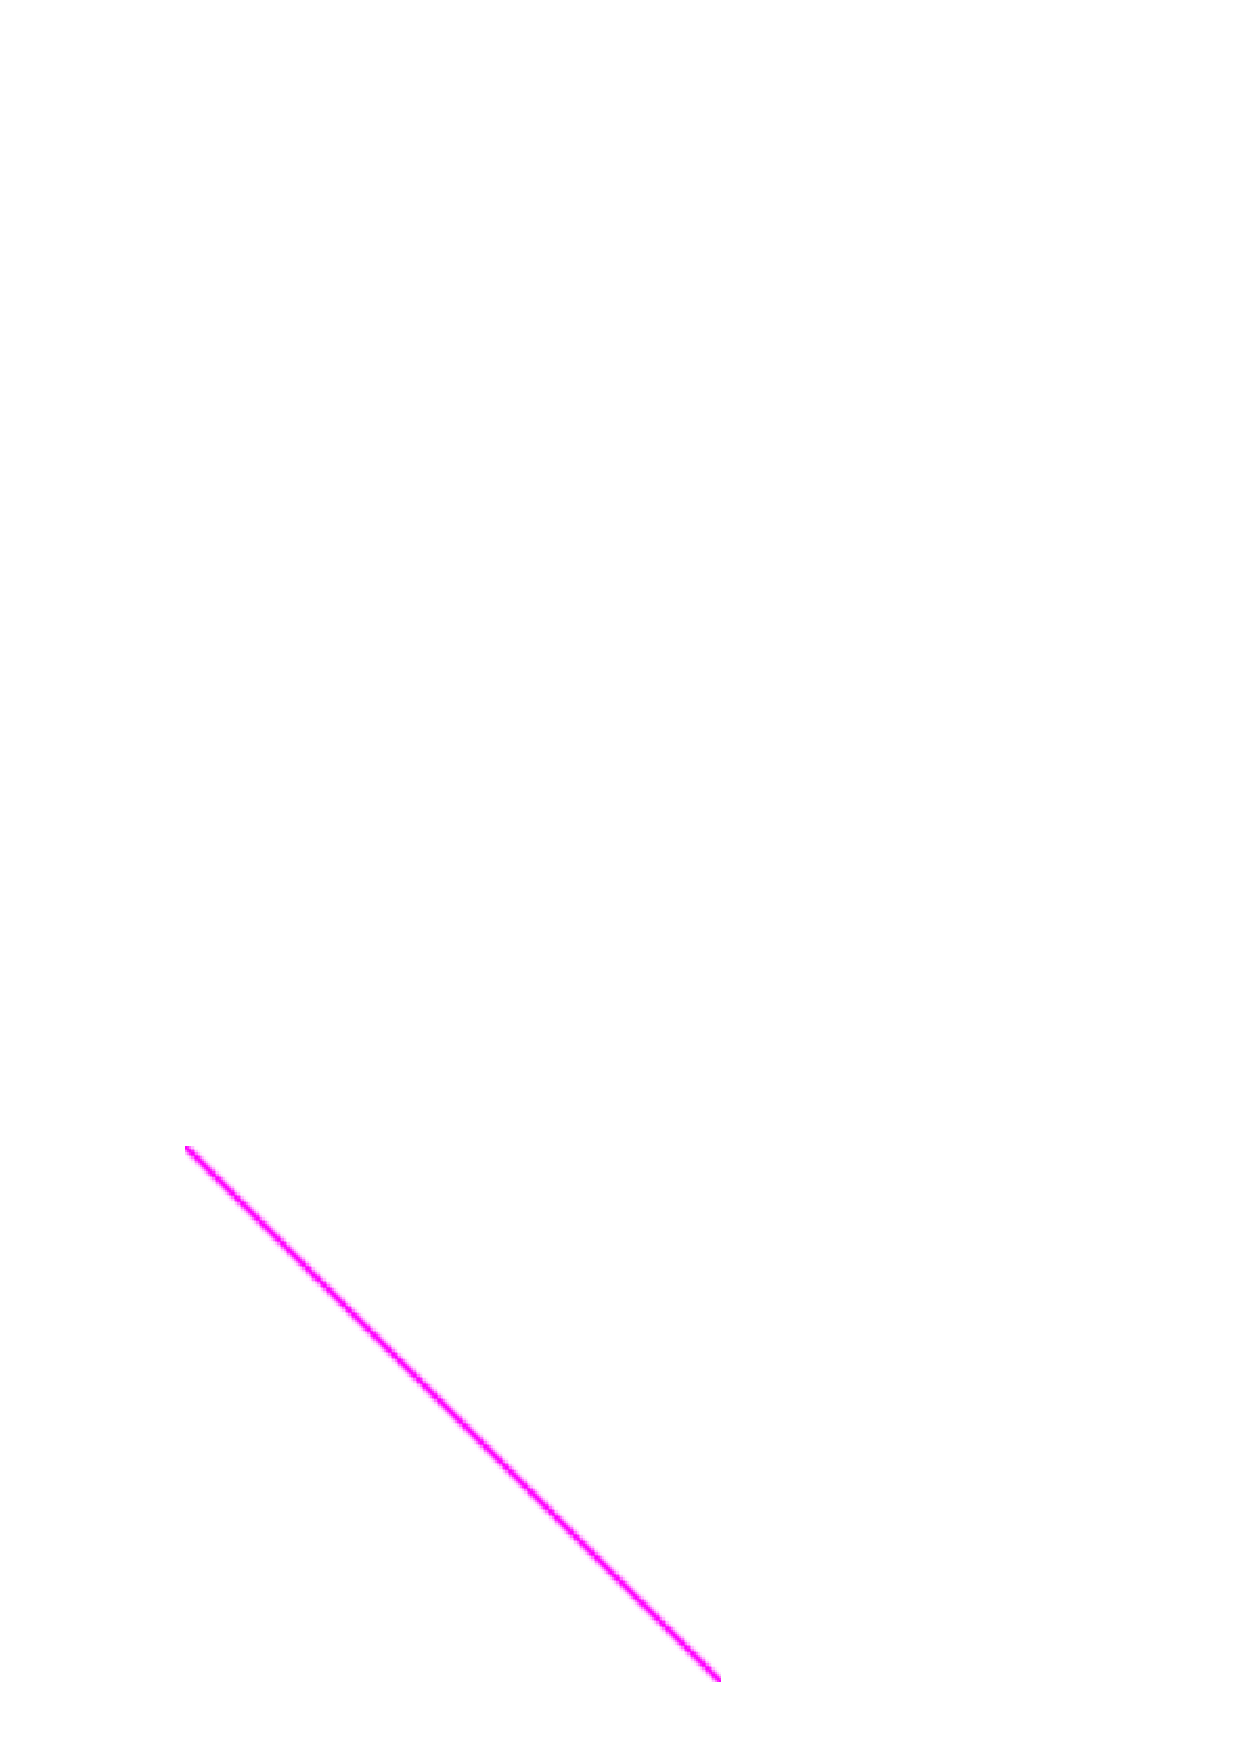
\includegraphics[width=\linewidth]{figure/fig4.2/evol-img-1.png}
		\end{mdframed}
	\end{minipage}
	\begin{minipage}{0.20\linewidth}
		\centering
		\begin{mdframed}
		    \includegraphics[width=\linewidth]{figure/fig4.2/evol-img-17.png}
		\end{mdframed}
	\end{minipage}
	\begin{minipage}{0.20\linewidth}
		\centering
		\begin{mdframed}
		    \includegraphics[width=\linewidth]{figure/fig4.2/evol-img-33.png}
		\end{mdframed}
	\end{minipage}
	\begin{minipage}{0.20\linewidth}
		\centering
		\begin{mdframed}
		    \includegraphics[width=\linewidth]{figure/fig4.2/evol-img-50.png}
		\end{mdframed}
	\end{minipage}
	%\qquad
	\vspace{1em}
	
	\begin{minipage}{0.20\linewidth}
		\centering
		\includegraphics[width=0.95\linewidth]{figure/fig4.2/evol-3d-1.png}
		\caption*{$\varepsilon = 1$}
	\end{minipage}
	\begin{minipage}{0.20\linewidth}
		\centering
		\includegraphics[width=0.95\linewidth]{figure/fig4.2/evol-3d-17.png}
		\caption*{$\varepsilon = 10^{-1}$}
	\end{minipage}
	\begin{minipage}{0.20\linewidth}
		\centering
		\includegraphics[width=0.95\linewidth]{figure/fig4.2/evol-3d-33.png}
		\caption*{$\varepsilon = 10^{-2}$}
	\end{minipage}
	\begin{minipage}{0.20\linewidth}
		\centering
		\includegraphics[width=0.95\linewidth]{figure/fig4.2/evol-3d-50.png}
		\caption*{$\varepsilon = 10^{-3}$}
	\end{minipage}
	
	\vspace{1em}
	\caption{注记4.2的可视化。以一维的具有密度函数的概率测度为例(输入测度见图4.4),给出不同$\varepsilon$下耦合子的三维图像和俯视图(颜色深度表示耦合子的分布密度),其收敛于原始最优传输问题的熵最大解。}
	\label{图4.3}
\end{figure}

类似(4.7),问题(4.9)也可以被表述为一个投影问题:
\begin{equation}
    \label{4.11}
    \min\limits_{\pi\in\mathcal{U}(\alpha,\beta)} \; \text{KL}(\pi|\mathcal{K})
\end{equation}

其中$\mathcal{K}$是Gibbs分布,$\text{d}\mathcal{K}(x,y)\overset{\text{def}}{=} e^{-\frac{c(x,y)}{\varepsilon}}\text{d}\alpha(x)\text{d}\beta(y)$。。当$\varepsilon\to 0$时,(4.11)的唯一解收敛于问题(2.15)的熵最大解,其证明见[L\'onard, 2012, Carlier等人, 2017]。

\begin{postulate}[交互熵]
类似于(2.16),我们可以从随机变量的角度来重述(4.9)
\begin{equation*}
    \mathcal{L}_c^\varepsilon(\alpha,\beta)\overset{\text{def}}{=}\min\limits_{(X,Y)} \left\{ \mathbb{E}_{(X,Y)}(c(X,Y))+\varepsilon I(X,Y):X\sim \alpha, Y\sim \beta \right\}
\end{equation*}

我们记$\pi$为$(X,Y)$的联合分布,$I(X,Y)\overset{\text{def}}{=} \text{KL}(\pi|\alpha \otimes \beta)$就是随机变量之间所谓的“交互信息”。不难证明,$I(X,Y)\geq 0$,且$I(X,Y)=0$当且仅当两个随机变量是独立的。
\end{postulate}

\begin{postulate}[独立性与耦合子]
一个耦合子$\pi\in\mathcal{U}(\alpha,\beta)$描述了$(\mathcal{X,Y})$空间中随机变量$(X,Y)$的联合分布,其中$X\sim \alpha,Y\sim \beta$。命题4.1对一般的测度也成立,即问题(4.9)的解$\pi_\varepsilon$当$\varepsilon\to+\infty$时收敛于耦合子$\alpha \otimes \beta$。耦合子$\alpha\otimes \beta$对应于$(X,Y)$独立的情形。另一方面,当$\varepsilon\to 0$时,$\pi_\varepsilon$收敛于原始最优传输问题(2.15)的某个解$\pi_0$。当$\mathcal{X}=\mathcal{Y}=\mathbb{R}^d$时,若$\alpha$与$\beta$具有关于勒贝格测度的密度函数,如注记2.24所说的情况,$\pi_0$是唯一的,并且支点集是蒙日映射$T:\mathbb{R}^d\to\mathbb{R}^d$的图像$(x,T(x))$。在这个情况下,$(X,Y)$从某种意义上说是完全依赖的,因为$Y=T(X)$且$X=T^{-1}(Y)$。在简单的一维情形$d=1$中,可以很方便地将$X$与$Y$的依赖关系可视化,需要用到关于联合分布$\pi$的连系函数$\xi_\pi$。首先(2.34)中定义的累积函数可以推广到耦合子上:
\begin{equation*}
    \forall (x,y)\in \mathbb{R}^2, \quad \mathcal{C}_\pi(x,y) \overset{\text{def}}{=} \int_{-\infty}^x\int_{-\infty}^y \text{d}\pi
\end{equation*}

连系函数定义为:
\begin{equation*}
    \forall (s,t)\in [0,1]^2, \quad \xi_\pi(s,t) \overset{\text{def}}{=} \mathcal{C}_\pi(\mathcal{C}_\alpha^{-1}(s),\mathcal{C}_{\beta}^{-1}(t))
\end{equation*}

其中累积函数的伪逆定义见(2.35)。对于独立的随机变量,$\varepsilon=+\infty$,即$\pi=\alpha\otimes \beta$,我们有$\xi_{\pi_{+\infty}}(s,t)=st$。另一方面,对于完全依赖的随机变量,$\varepsilon=0$,我们有$\xi_{\pi_0}(s,t)=\min(s,t)$。图4.4展示了熵正则化诱导的连系函数$\xi_{\pi_\varepsilon}$,包括上述两个极端情况和二者之间的情况。
\end{postulate}

\begin{figure}[H]
	\centering
	\begin{minipage}{0.8\linewidth}
	
	\centering
	\begin{minipage}{0.40\linewidth}
		\centering
		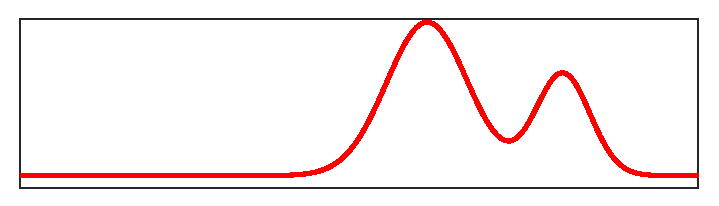
\includegraphics[width=0.95\linewidth]{figure/fig4.4/input-1.eps}
		\caption*{$\alpha$}
	\end{minipage}
	\begin{minipage}{0.40\linewidth}
		\centering
		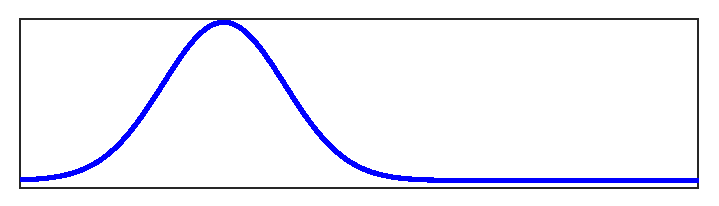
\includegraphics[width=0.95\linewidth]{figure/fig4.4/input-2.eps}
		\caption*{$\beta$}
	\end{minipage}
	%\qquad
	\vspace{1em}
	
	\begin{minipage}{0.19\linewidth}
		\centering
		\begin{mdframed}
		    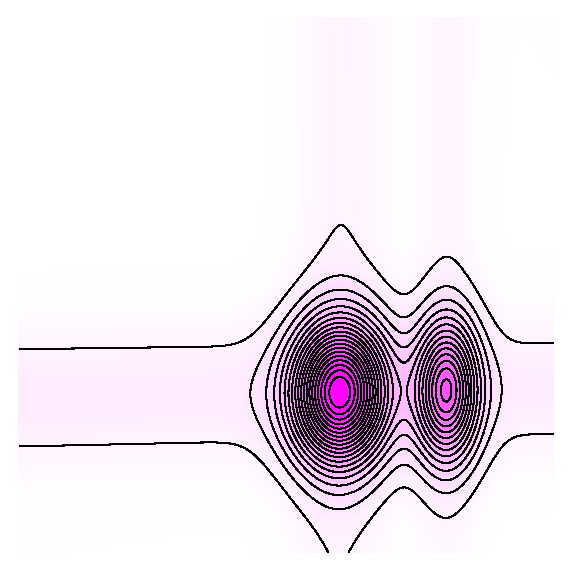
\includegraphics[width=\linewidth]{figure/fig4.4/evol-levelsets-1.eps}
		\end{mdframed}
	\end{minipage}
	\begin{minipage}{0.19\linewidth}
		\centering
		\begin{mdframed}
		    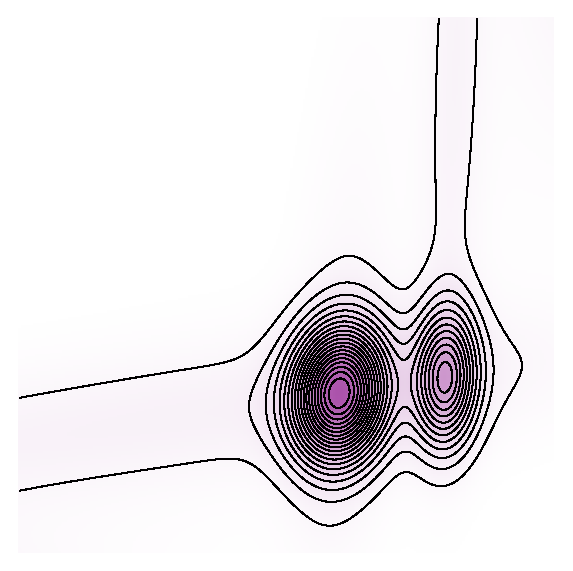
\includegraphics[width=\linewidth]{figure/fig4.4/evol-levelsets-17.eps}
		\end{mdframed}
	\end{minipage}
	\begin{minipage}{0.19\linewidth}
		\centering
		\begin{mdframed}
		    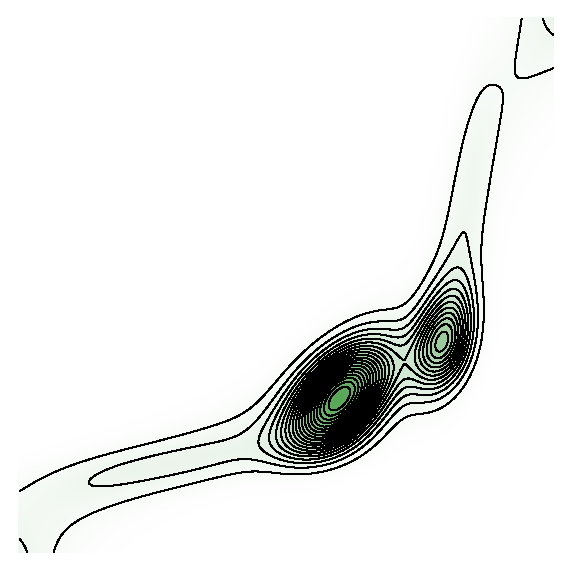
\includegraphics[width=\linewidth]{figure/fig4.4/evol-levelsets-33.eps}
		\end{mdframed}
	\end{minipage}
	\begin{minipage}{0.19\linewidth}
		\centering
		\begin{mdframed}
		    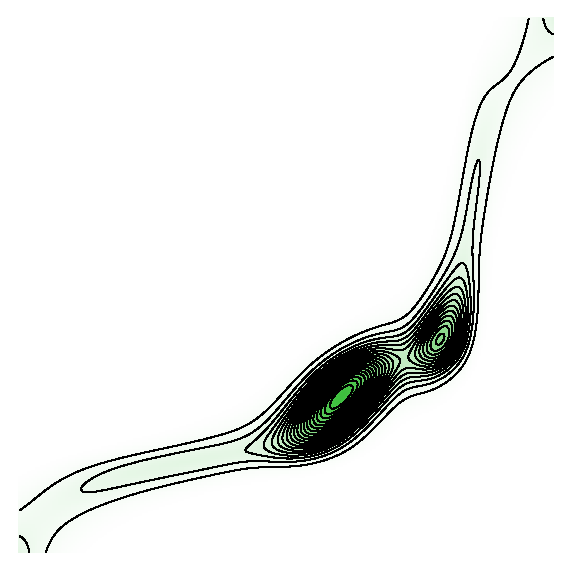
\includegraphics[width=\linewidth]{figure/fig4.4/evol-levelsets-38.eps}
		\end{mdframed}
	\end{minipage}
	\begin{minipage}{0.19\linewidth}
		\centering
		\begin{mdframed}
		    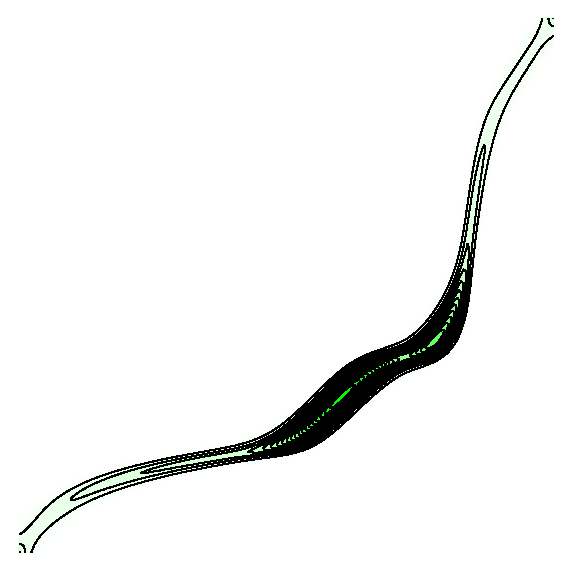
\includegraphics[width=\linewidth]{figure/fig4.4/evol-levelsets-50.eps}
		\end{mdframed}
	\end{minipage}
	%\qquad
	\vspace{1em}
	
	\begin{minipage}{0.19\linewidth}
		\centering
		\begin{mdframed}
		    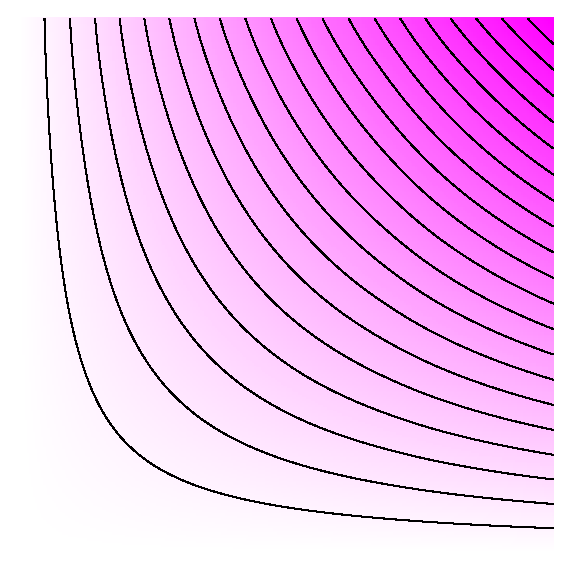
\includegraphics[width=\linewidth]{figure/fig4.4/evol-copula-1.eps}
		\end{mdframed}
		\caption*{$\varepsilon = 1$}
	\end{minipage}
	\begin{minipage}{0.19\linewidth}
		\centering
		\begin{mdframed}
		    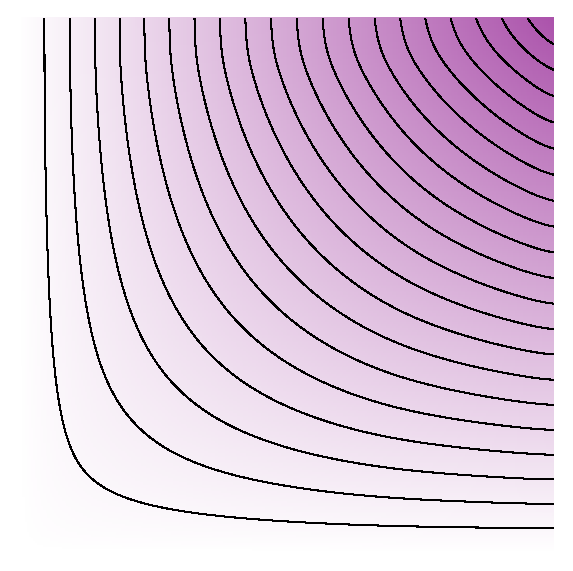
\includegraphics[width=\linewidth]{figure/fig4.4/evol-copula-17.eps}
		\end{mdframed}
		\caption*{$\varepsilon = 10^{-1}$}
	\end{minipage}
	\begin{minipage}{0.19\linewidth}
		\centering
		\begin{mdframed}
		    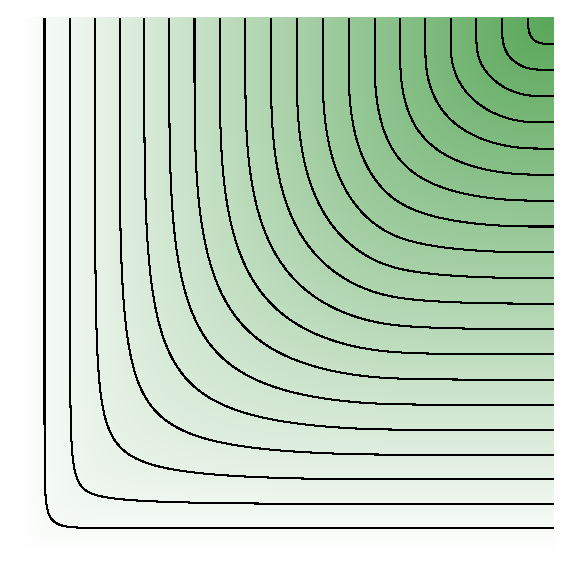
\includegraphics[width=\linewidth]{figure/fig4.4/evol-copula-33.eps}
		\end{mdframed}
		\caption*{$\varepsilon = 10^{-2}$}
	\end{minipage}
	\begin{minipage}{0.19\linewidth}
		\centering
		\begin{mdframed}
		    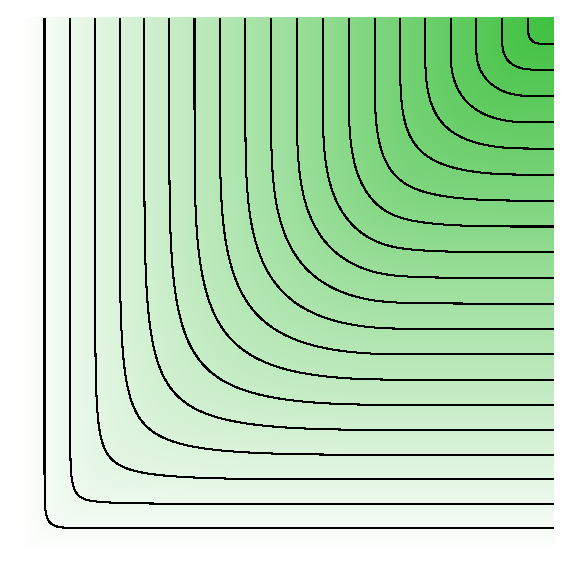
\includegraphics[width=\linewidth]{figure/fig4.4/evol-copula-38.eps}
		\end{mdframed}
		\caption*{$\varepsilon = 5\times 10^{-3}$}
	\end{minipage}
	\begin{minipage}{0.19\linewidth}
		\centering
		\begin{mdframed}
		    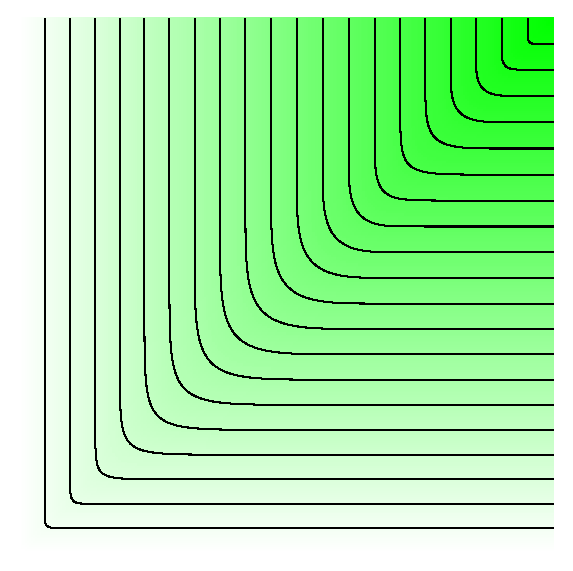
\includegraphics[width=\linewidth]{figure/fig4.4/evol-copula-50.eps}
		\end{mdframed}
		\caption*{$\varepsilon = 10^{-3}$}
	\end{minipage}
	
	\end{minipage}
	
	\vspace{1em}
	\caption{第一行:输入测度;第二行:问题(4.9)在不同$\varepsilon$下的解$\pi_\varepsilon$;第三行:$\pi_\varepsilon$对应的连系函数$\xi_{\pi_\varepsilon}$}
	\label{图4.4}
\end{figure}

\section{Sinkhorn算法及其收敛性}

下面这个命题表明,问题(4.2)的解可以被参数化为$n+m$个变量。从某种意义上说,这种参数化本质上是对偶化,因为$\mathbf{P}\in\mathbf{U(a,b)}$具有$nm$个变量但只有$n+m$条约束。

\begin{proposition}
问题(4.2)的解是唯一的,并且可以表示成下述形式:
\begin{equation}
    \label{4.12}
    \forall (i,j)\in \mathbb{[}n\mathbb{]}\times \mathbb{[}m\mathbb{]}, \quad \mathbf{P}_{i,j}=\mathbf{u}_i\mathbf{K}_{i,j}\mathbf{v}_j
\end{equation}

其中参数$(\mathbf{u,v})\in \mathbb{R}_+^n \times \mathbb{R}_+^m$,$\mathbf{K}$是关于代价矩阵$\mathbf{C}$的Gibbs核
\end{proposition}

\begin{proof}
我们引入对偶变量,对应于每条行和、列和约束,则(4.2)的拉格朗日函数为:
\begin{equation*}
    \mathcal{E}(\mathbf{P,f,g}) = \langle \mathbf{P,C} \rangle - \varepsilon \mathbf{H(P)} - \langle \mathbf{f}, \mathbf{P}\mathbbm{1}_m-\mathbf{a} \rangle - \langle \mathbf{g}, \mathbf{P}^T \mathbbm{1}_n - \mathbf{b} \rangle
\end{equation*}

由一阶必要性条件可得:
\begin{equation*}
    \frac{\partial \mathcal{E}(\mathbf{P,f,g})}{\partial \mathbf{P}_{i,j}} = \mathbf{C}_{i,j} + \varepsilon \log(\mathbf{P}_{i,j}) - \mathbf{f}_i - \mathbf{g}_j = 0
\end{equation*}

从而正则化问题(4.2)的解$\mathbf{P}$各元素为$\mathbf{P}_{i,j}=e^{\mathbf{f}_i/\varepsilon}e^{-\mathbf{C}_{i,j}/\varepsilon}e^{\mathbf{g}_j/\varepsilon}$,这可以用非负向量$\mathbf{u,v}$表示为(4.12)中所述形式,即得证。
\end{proof}

\vspace{1.5em}

\textbf{Sinkhorn算法.} 式(4.12)可以方便地表述为矩阵形式:$\mathbf{P}=\text{diag}(\mathbf{u})\mathbf{K}\text{diag}(\mathbf{v})$。考虑到$\mathbf{U(a,b)}$的质量守恒约束,向量$\mathbf{u,v}$因此必须满足下述非线性约束:
\begin{equation}
    \label{4.13}
    \text{diag}(\mathbf{u})\mathbf{K}\text{diag}(\mathbf{v})\mathbbm{1}_m=\mathbf{a} \quad \text{and} \quad \text{diag}(\mathbf{v})\mathbf{K}^T\text{diag}(\mathbf{u})\mathbbm{1}_n=\mathbf{b}
\end{equation}

注意到$\text{diag}(\mathbf{v})\mathbbm{1}_m=\mathbf{v}$,我们可以将上式写为更简单的形式:
\begin{equation}
    \label{4.14}
    \mathbf{u}\odot (\mathbf{Kv}) = \mathbf{a} \quad \text{and} \quad \mathbf{v}\odot (\mathbf{K}^T\mathbf{u}) = \mathbf{b}
\end{equation}

其中$\odot$是两向量各分量对应相乘。这为问题的求解提供了一种灵感,即迭代地利用上述两式更新$\mathbf{u,v}$:
\begin{equation}
    \label{4.15}
    \mathbf{u}^{(\ell+1)} \overset{\text{def}}{=} \frac{\mathbf{a}}{\mathbf{Kv}^{(\ell)}} \quad \text{and} \quad \mathbf{v}^{(\ell+1)} \overset{\text{def}}{=} \frac{\mathbf{b}}{\mathbf{K}^T\mathbf{u}^{(\ell+1)}}
\end{equation}

其中除法是指各分量对应相除,并取初始值$\mathbf{v}^{(0)}=\mathbbm{1}_m$。这就是Sinkhorn算法。事实上不同的初值可能会得到不同的解$\mathbf{u,v}$,这是因为只要$(\mathbf{u,v})$满足(4.13)式,则$(\lambda \mathbf{u}, \mathbf{v}/\lambda)\;(\lambda>0)$也满足(4.13),但这并不影响正则化问题的最终解$\text{diag}(\mathbf{u})\mathbf{K}\text{diag}(\mathbf{v})$。从图4.5可以看到,随着Sinkhorn算法迭代的进行,当前步的耦合子$\pi_\varepsilon^{(\ell)}$从对角线开始,被逐步“推”至正则化问题最优解$\pi_\varepsilon$。

\begin{figure}[H]
	\centering
	\begin{minipage}{0.8\linewidth}
	\centering
	\begin{minipage}{0.16\linewidth}
		\centering
		\begin{mdframed}
		    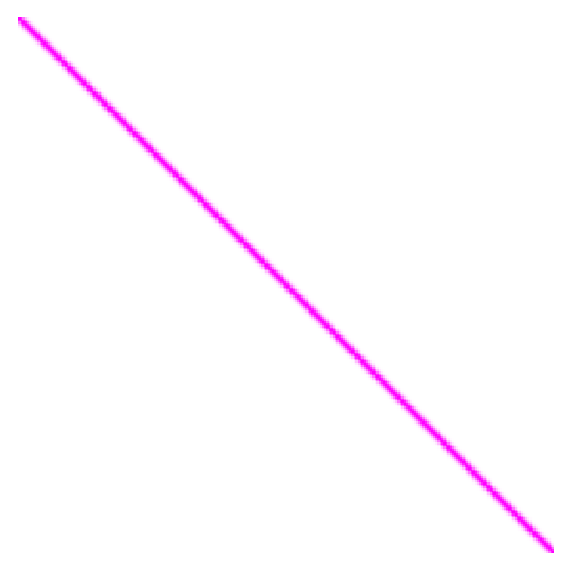
\includegraphics[width=\linewidth]{figure/fig4.5/evol-img-1.eps}
		\end{mdframed}
		\caption*{$\ell=0$}
	\end{minipage}
	\begin{minipage}{0.16\linewidth}
		\centering
		\begin{mdframed}
		    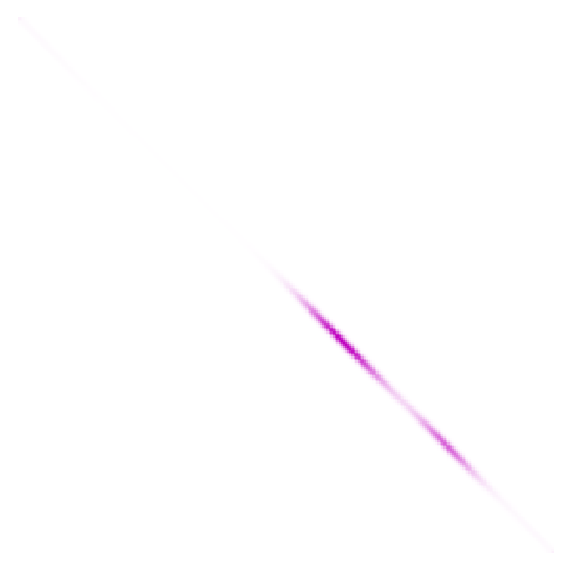
\includegraphics[width=\linewidth]{figure/fig4.5/evol-img-2.eps}
		\end{mdframed}
		\caption*{$\ell=1$}
	\end{minipage}
	\begin{minipage}{0.16\linewidth}
		\centering
		\begin{mdframed}
		    \includegraphics[width=\linewidth]{figure/fig4.5/evol-img-3.eps}
		\end{mdframed}
		\caption*{$\ell=10$}
	\end{minipage}
	\begin{minipage}{0.16\linewidth}
		\centering
		\begin{mdframed}
		    \includegraphics[width=\linewidth]{figure/fig4.5/evol-img-4.eps}
		\end{mdframed}
		\caption*{$\ell=100$}
	\end{minipage}
	\begin{minipage}{0.16\linewidth}
		\centering
		\begin{mdframed}
		    \includegraphics[width=\linewidth]{figure/fig4.5/evol-img-5.eps}
		\end{mdframed}
		\caption*{$\ell=1000$}
	\end{minipage}
	\begin{minipage}{0.16\linewidth}
		\centering
		\begin{mdframed}
		    \includegraphics[width=\linewidth]{figure/fig4.5/evol-img-6.eps}
		\end{mdframed}
		\caption*{$\ell=5000$}
	\end{minipage}
	\end{minipage}
	%\qquad
	\vspace{.5em}
	\caption{Sinkhorn迭代过程中的耦合子$\pi_\varepsilon^{(\ell)}$图像,输入测度与图4.4相同}
	\label{图4.5}
\end{figure}

\begin{postulate}[研究历史]
迭代格式(4.15)在[Yule, 1912, Kruithof, 1937]中首次出现,后来通过迭代比例拟合算法[Deming and Stephan, 1940]和RAS法[Bacharach, 1965]而被人们熟知。这个迭代的收敛性由Sinkhorn在1964年证明,这也是其得名原因。这个算法后来被Ruschendorn[1995]推广至无穷维。在其特殊情形最优分配中,它被重命名为“软分配法”[Kosowskyh and Yuille, 1994],它可以用于求解经济学中的一些匹配问题[Galichon and Salani\'e, 2009]。近年来,随着Cuturi在2013年发现Sinkhorn算法能高效地给出近似精度令人满意的最优传输解,熵正则化在数据科学中获得了新的关注。得益于无缝并行化技术,我们可以同时求解若干个最优传输问题(尤其是利用GPU运算,见注记4.16)。Sinkhorn算法还有很多的推广和扩展,例如当$\mathbf{a=b}$时,我们可以使用均值投影迭代来保持对称性[Knight等人, 2014]。
\end{postulate}

\begin{postulate}[总体复杂度]
一份详细的复杂度分析[Altschuler等人, 2017]表明(出于简洁考虑,设$n=m$),取$\varepsilon=\frac{\tau}{4\log(n)}$,则Sinkhorn算法只需要$O(||\mathbf{C}||_\infty^3 \log(n) \tau^{-3})$次迭代步就能让得到的解$\mathbf{\hat{P}}\in\mathbf{U(a,b)}$满足$\tau$-近似性,即$\langle \mathbf{\hat{P}}, \mathbf{C} \rangle \leq L_\mathbf{C}(\mathbf{a,b})+\tau$
\end{postulate}

\begin{postulate}[Sinkhorn算法的数值稳定性]
随着$\varepsilon \to 0$,Sinkhorn算法收敛需要的时间越长,数值稳定性也会受到影响。这是因为一旦$\mathbf{K}$中的元素过小,计算机将无法存储从而将其视为$0$,于是在Sinkhorn迭代过程中出现除$0$的情况。要想解决这个原因导致的数值不稳定,需要引入对数化算法,这将在注记4.18中详细说明
\end{postulate}

\begin{postulate}[Bregman迭代投影法]
我们记
\begin{equation*}
    \mathcal{C}_\mathbf{a}^1 \overset{\text{def}}{=} \{ \mathbf{P}\; : \; \mathbf{P}\mathbbm{1}_m=\mathbf{a} \} \quad \text{and} \quad \mathcal{C}_\mathbf{b}^2 \overset{\text{def}}{=} \{ \mathbf{P}\; : \; \mathbf{P}^T\mathbbm{1}_n=\mathbf{b} \}
\end{equation*}

行和与列和约束即可表述为$\mathbf{U(a,b)} = \mathcal{C}_\mathbf{a}^1 \cap \mathcal{C}_\mathbf{b}^2$。我们有Bregman迭代投影法[Bregman, 1967]:
\begin{equation}
    \label{4.16}
    \mathbf{P}^{(\ell + 1)} \overset{\text{def}}{=} \text{Proj}_{\mathcal{C}_\mathbf{a}^1}^{\mathbf{KL}} (\mathbf{P}^{(\ell)}) \quad \text{and} \quad \mathbf{P}^{(\ell + 2)} \overset{\text{def}}{=} \text{Proj}_{\mathcal{C}_\mathbf{b}^2}^{\mathbf{KL}} (\mathbf{P}^{(\ell + 1)})
\end{equation}

由于$\mathcal{C}_\mathbb{a}^1$与$\mathcal{C}_\mathbb{b}^2$是仿射集,故上述迭代会收敛于(4.7)的解,具体见[Bregman, 1967]。事实上这个迭代与Sinkhorn迭代(4.15)是等价的,我们可以定义:
\begin{equation*}
    \mathbf{P}^{(2\ell)} \overset{\text{def}}{=} \text{diag}(\mathbf{u}^{(\ell)}) \mathbf{K} \text{diag}(\mathbf{v}^{(\ell)})
\end{equation*}

不难得到:
\begin{equation*}
    \mathbf{P}^{(2\ell+1)} \overset{\text{def}}{=} \text{diag}(\mathbf{u}^{(\ell+1)}) \mathbf{K} \text{diag}(\mathbf{v}^{(\ell)}) \quad \text{and} \quad  \mathbf{P}^{(2\ell+2)} \overset{\text{def}}{=} \text{diag}(\mathbf{u}^{(\ell+1)}) \mathbf{K} \text{diag}(\mathbf{v}^{(\ell+1)})
\end{equation*}

在实际应用中,我们还是愿意使用(4.15),因为它只要用到矩阵与向量操作,很容易利用GPU加速。
\end{postulate}

\begin{postulate}[邻近点算法]
我们可以对KL背离度使用所谓的邻近点算法来获得无正则化($\varepsilon$)问题(2.11)的解。我们定义$F(\mathbf{P})\overset{\text{def}}{=}\langle \mathbf{P,C} \rangle + \iota_{\mathbf{U(a,b)}}(\mathbf{P})$为无正则优化项。KL背离度的邻近点算法将计算$F$的极小值点,也就是无正则化最优传输问题(2.11)的解。迭代地进行:
\begin{equation}
    \label{4.17}
    \mathbf{P}^{(\ell +1)}\overset{\text{def}}{=} \text{Prox}^{\mathbf{KL}}_{\frac{1}{\varepsilon}F}(\mathbf{P}^{(\ell)}) \overset{\text{def}}{=} \text{argmin}\limits_{\mathbf{P}\in\mathbb{R}_+^{n\times m}}\mathbf{KL}(\mathbf{P}|\mathbf{P}^{(\ell)})+\frac{1}{\varepsilon}F(\mathbf{P})
\end{equation}

从任意的初值$\mathbf{P}^{(0)}$开始迭代。邻近点算法是最基本的邻近分离方法。它一开始是在欧式度量中被引入的[Rockafellar, 1976],可以扩展至任意的Bregman背离度[Censor and Zenios, 1992],尤其是在KL背离度中应用。邻近点算法的prox操作通常不具有闭形式,因此需要一些子迭代。式(4.17)中的优化和熵正则化问题(4.2)非常相似,相当于把熵正则项$-\mathbf{H}$替换成了KL背离度$\mathbf{KL}(\cdot|\mathbf{P}^{(\ell)})$。命题4.3和Sinkhorn迭代(4.15)可以归结为这个更一般的形式,我们设Gibbs核为$\mathbf{K}=e^{-\frac{\mathbf{C}}{\varepsilon}}\odot \mathbf{P}^{(\ell)}$。从而迭代式(4.17)可以用Sinkhorn算法来实现。设$\mathbf{P}^{(0)}=\mathbbm{1}_n\mathbbm{1}_m^T$,迭代即可写为下述形式:
\begin{align*}
    \mathbf{P}^{(\ell+1)} &= \text{diag}(\mathbf{u}^{(\ell)})(e^{-\frac{\mathbf{C}}{\varepsilon}}\odot \mathbf{P}^{(\ell)})\text{diag}(\mathbf{v}^{(\ell)})\\
    &= \text{diag}(\mathbf{u}^{(\ell)}\odot \cdots \odot \mathbf{u}^{(0)})(e^{-\frac{(\ell+1)\mathbf{C}}{\varepsilon}}\odot \mathbf{P}^{(\ell)})\text{diag}(\mathbf{v}^{(\ell)}\odot \cdots \odot \mathbf{v}^{(0)})
\end{align*}

因此迭代中的Prox操作可以由Sinkhorn算法计算,核为$e^{-\frac{\mathbf{C}}{\varepsilon/\ell}}$,即增加了一个正则衰减参数$\varepsilon/\ell$。这个方法和Sinkhorn算法在正则衰减方案中的应用研究是紧密相关的,例如见[Kosowsky and Yuille, 1994]。在低维空间中,用这个方法结合多重网格策略去近似自适应稀疏网格,是非常高效的[Schmitzer, 2016b]。
\end{postulate}

\begin{postulate}[其它形式的正则化]
式(4.2)中的熵正则化项$-\mathbf{H(P)}$可以替换为任意的严格凸惩罚项$R(\mathbf{P})$,例如见[Dessein等人, 2018]。一种典型的例子是使用平方$\ell^2$范数:
\begin{equation}
    \label{4.18}
    R(\mathbf{P}) = \sum_{i,j} \mathbf{P}_{i,j}^2 + \iota_{\mathbb{R}_+}(\mathbf{P}_{i,j})
\end{equation}

换言之,我们考虑如下的平方正则化问题:
\begin{equation*}
    \min\limits_{\mathbf{P}\in\mathbf{U(a,b)}} \quad \langle \mathbf{P,C} \rangle + \varepsilon \sum_{i,j} \mathbf{P}_{i,j}^2
\end{equation*}

详见[Essid and Solomon, 2017]。它的主要好处是对稀疏的(指除少数位置外,其余位置均小于某个阈值)耦合矩阵更加友好,但代价是不能像Sinkhorn算法一样并行计算多个问题。图4.6是两种正则化方法得到的近似解对比。另一类正则化的例子是Tsallis熵[Muzellec等人, 2017]。
\end{postulate}

\begin{figure}[H]
	\centering
	\begin{minipage}{0.8\linewidth}
	\centering
	\begin{minipage}{0.19\linewidth}
		\centering
		    \includegraphics[width=\linewidth]{figure/fig4.6/1.png}
		\caption*{$\varepsilon=1$}
	\end{minipage}
	\begin{minipage}{0.19\linewidth}
		\centering
		    \includegraphics[width=\linewidth]{figure/fig4.6/2.png}
		\caption*{$\varepsilon=10^{-1}$}
	\end{minipage}
	\begin{minipage}{0.19\linewidth}
		\centering
		    \includegraphics[width=\linewidth]{figure/fig4.6/3.png}
		\caption*{$\varepsilon=5\times 10^{-2}$}
	\end{minipage}
	\begin{minipage}{0.19\linewidth}
		\centering
		    \includegraphics[width=\linewidth]{figure/fig4.6/4.png}
		\caption*{$\varepsilon=5\times 10^{-3}$}
	\end{minipage}
	\begin{minipage}{0.19\linewidth}
		\centering
		    \includegraphics[width=\linewidth]{figure/fig4.6/5.png}
		\caption*{$\varepsilon=10^{-3}$}
	\end{minipage}
	\vspace{.5em}
	\begin{minipage}{0.19\linewidth}
		\centering
		    \includegraphics[width=\linewidth]{figure/fig4.6/6.png}
		\caption*{$\varepsilon=5\times 10^3$}
	\end{minipage}
	\begin{minipage}{0.19\linewidth}
		\centering
		    \includegraphics[width=\linewidth]{figure/fig4.6/7.png}
		\caption*{$\varepsilon=10^3$}
	\end{minipage}
	\begin{minipage}{0.19\linewidth}
		\centering
		    \includegraphics[width=\linewidth]{figure/fig4.6/8.png}
		\caption*{$\varepsilon=10^2$}
	\end{minipage}
	\begin{minipage}{0.19\linewidth}
		\centering
		    \includegraphics[width=\linewidth]{figure/fig4.6/9.png}
		\caption*{$\varepsilon=10$}
	\end{minipage}
	\begin{minipage}{0.19\linewidth}
		\centering
		    \includegraphics[width=\linewidth]{figure/fig4.6/10.png}
		\caption*{$\varepsilon=1$}
	\end{minipage}
	\end{minipage}
	%\qquad
	\vspace{.5em}
	\caption{熵正则化(上行)与平方正则化(下行)的对比,图中展示的是不同$\varepsilon$下正则化问题的解}
	\label{图4.6}
\end{figure}

\begin{postulate}[质心投影]
康托洛维奇问题(2.11)和它的熵正则化问题(4.2)都给出了一个耦合子$\mathbf{P}\in\mathbf{U(a,b)}$。为了定义出传输映射$T:\mathcal{X}\to\mathcal{Y}$,其中$\mathcal{Y}=\mathbb{R}^d$,我们可以定义所谓的质心投影映射:
\begin{equation}
    \label{4.19}
    T:x_i\in\mathcal{X} \mapsto \frac{1}{\mathbf{a}_i}\sum_j \mathbf{P}_{ij}y_j \in \mathcal{Y}
\end{equation}

其中输入测度具有(2.3)的形式,注意$T$只在$\alpha$的支点集$(x_i)_i$中有定义。当$\mathbf{P}$是置换矩阵时,$T$就是蒙日映射,若该蒙日映射解是唯一的,则当$\varepsilon\to 0$时,正则化问题解的质心投影映射会收敛于它。对于一般的测度,问题(2.15)及其正则化(4.9)给出耦合子$\pi\in\mathcal{U}(\alpha,\beta)$。注意到耦合子$\pi$关于$\alpha\otimes \beta$的相对密度$\frac{\text{d}\pi(x,y)}{\text{d}\alpha(x)\text{d}\beta(y)}$总是存在的,因此下式可以诱导出一个映射:
\begin{equation}
    \label{4.20}
    T:x\in\mathcal{X} \mapsto \int_\mathcal{Y} y \frac{\text{d}\pi(x,y)}{\text{d}\alpha(x)\text{d}\beta(y)} \text{d}\beta(y)
\end{equation}

当$\varepsilon=0$时,$\pi$的支点为蒙日映射的图像,当$\varepsilon>0$时,上式给出蒙日映射的光滑近似。它可以被用于计算概率测度空间(采用瓦瑟斯坦距离度量)的近似主测地线[Seguy and Cuturi, 2015]。
\end{postulate}

\begin{postulate}[希尔伯特距离]
文献[Franklin and Lorenz, 1989]首次提出,使用$\mathbb{R}_{+,*}^n$上的希尔伯特距离能大大简化Sinkhorn算法的全局收敛性分析,其定义如下:
\begin{equation*}
    \forall (\mathbf{u,u'})\in(\mathbb{R}_{+,*}^n)^2, \quad d_\mathcal{H}(\mathbf{u,u'})\overset{\text{def}}{=} \log \max\limits_{i,j} \frac{\mathbf{u}_i\mathbf{u}_j'}{\mathbf{u}_j\mathbf{u}_i'}
\end{equation*}

可以证明,它是(正)射影锥$\mathbb{R}_{+,*}^n/\sim$上的距离度量,其中等价关系定义为:$\mathbf{u}\sim \mathbf{u'}$,若$\exists r>0, \mathbf{u}=r\mathbf{u'}$。这意味着$d_\mathcal{H}$满足三角不等式,且$d_\mathcal{H}(\mathbf{u,u'})=0$当且仅当$\mathbf{u}=\mathbf{u'}$。这其实就是有界凸开集上的希尔伯特距离度量[Hilbert, 1895]的射影版本。在这个距离度量下,射影锥$\mathbb{R}_{+,*}^n/\sim$是完备度量空间。通过对变量进行对数变换,我们可以得到,射影锥上的希尔伯特距离与变分半范数同构,即:
\begin{equation}
    \label{4.21}
    d_\mathcal{H}(\mathbf{u,u'}) = ||\log(\mathbf{u})-\log(\mathbf{u'})||_{\text{var}}
\end{equation}
\begin{equation*}
    \text{其中} \quad ||\mathbf{f}||_{\text{var}}\overset{\text{def}}{=} (\max\limits_i \mathbf{f}_i) - (\min\limits_i \mathbf{f}_i)
\end{equation*}

变分半范数和$\ell^\infty$范数是密切相关的,我们总是有$||\mathbf{f}||_{\text{var}}\leq 2||\mathbf{f}||_\infty$。若$\mathbf{f}_i=0$对某个$i$成立,则也有$||\mathbf{f}||_\infty \leq ||\mathbf{f}||_{\text{var}}$。这些界的估计在Sinkhorn算法的收敛性分析(见下述注记4.14)中是非常有用的。事实上对于射影锥中的$\mathbf{u}$,由于相乘一个正常数不改变其等价类,因此$\mathbf{f}=\log(\mathbf{u})$在加减一个常数意义下也是等价的,所以我们总是可以假设存在$\mathbf{f}_i=0$。希尔伯特距离由[Birkhoff, 1957]和[Samelson等人, 1957]各自独立引入,他们证明了下述基本定理,表明正值矩阵是射影锥上的严格压缩映射。
\end{postulate}

\begin{theorem}
设$\mathbf{K}\in\mathbb{R}_{+,*}^{n\times m}$,则对任意$(\mathbf{v,v'})\in (\mathbb{R}_{+,*}^{m})^2$,有不等式:
\begin{equation*}
    d_\mathcal{H}(\mathbf{Kv,Kv'}) \leq \lambda(\mathbf{K})d_\mathcal{H}(\mathbf{v,v'}), \quad \text{其中} \;
         \lambda(\mathbf{K}) \overset{\text{def}}{=} \frac{\sqrt{\eta(\mathbf{K})}-1}{\sqrt{\eta(\mathbf{K})}+1} < 1, \;\;
         \eta(\mathbf{K}) \overset{\text{def}}{=} \max\limits_{i,j,k,l}\frac{\mathbf{K}_{i,k}\mathbf{K}_{j,l}}{\mathbf{K}_{j,k}\mathbf{K}_{i,l}}
\end{equation*}

图4.7直观地说明了这个定理。
\end{theorem}

\begin{figure}[H]
    \centering
    \includegraphics[width=0.7\textwidth]{figure/fig4.7.png}
    \caption{左图:射影锥上的希尔伯特距离。右图:正值矩阵是射影锥上的严格压缩映射。}
    \label{图4.7}
\end{figure}

\begin{postulate}[Perron-Frobenius定理]
定理4.1的一个典型应用是给出Perron-Frobenius定理的定量证明,我们在注记4.15将会解释,这与Sinkhorn迭代的局部线性化近似有关。一个满足$\mathbf{K}^T\mathbbm{1}_n=\mathbbm{1}_n$的矩阵$\mathbf{K}\in\mathbb{R}_+^{n\times n}$将$\Sigma_n$映射到$\Sigma_n$。若满足进一步条件$\mathbf{K}>0$,则根据定理4.1,它是射影锥上的严格压缩映射,因此存在唯一的不动点$p^\star \in \Sigma_n$满足$\mathbf{P}p^\star = p^\star$。进一步地,对任意$p_0i\in\Sigma_n$,有$d_\mathcal{H}(\mathbf{K}^\ell p_0, p^\star) \leq \lambda(\mathbf{K})^\ell d_\mathcal{H}(p_0,p^\star)$。即,矩阵$\mathbf{K}$定义的迭代具有线性收敛性,收敛于$p^\star$,如图4.8所示。
\end{postulate}

\begin{figure}[H]
    \centering
    \includegraphics[width=0.7\textwidth]{figure/fig4.8.png}
    \caption{线性收敛性:$\mathbf{K}^\ell \Sigma_3 \to \{p^\star\}$,其中$\mathbf{K}\in\mathbb{R}_+^{3\times 3}$满足$\mathbf{K}^T\mathbbm{1}_3=\mathbbm{1}_3$}
    \label{图4.8}
\end{figure}

\begin{postulate}[Sinkhorn算法的全局收敛性]
下述定理由[Franklin and Lorenz, 1989]证明,利用定理4.1证明了Sinkhorn迭代的线性收敛性。
\end{postulate}

\begin{theorem}
对于(4.15)定义的Sinkhorn迭代,我们有$(\mathbf{u}^{(\ell)},\mathbf{v}^{(\ell)})\to (\mathbf{u}^\star, \mathbf{v}^\star)$,且
\begin{equation}
    \label{4.22}
    d_\mathcal{H}(\mathbf{u}^{(\ell)},\mathbf{u}^\star) = O(\lambda(\mathbf{K})^{2\ell}), \quad d_\mathcal{H}(\mathbf{v}^{(\ell)},\mathbf{v}^\star) = O(\lambda(\mathbf{K})^{2\ell})
\end{equation}

此外,
\begin{equation}
    \label{4.23}
    \renewcommand{\arraystretch}{1.5}
    \begin{array}{l}
    d_\mathcal{H}(\mathbf{u}^{(\ell)},\mathbf{u}^\star) \leq \frac{d_\mathcal{H}(\mathbf{P}^{(\ell)}\mathbbm{1}_m, \mathbf{a})}{1-\lambda(\mathbf{K})^2} \\ 
    d_\mathcal{H}(\mathbf{v}^{(\ell)},\mathbf{v}^\star) \leq \frac{d_\mathcal{H}(\mathbf{P}^{(\ell)T}\mathbbm{1}_n, \mathbf{b})}{1-\lambda(\mathbf{K})^2}
    \end{array}
\end{equation}

其中$\mathbf{P}^{(\ell)}\overset{\text{def}}{=}\text{diag}(\mathbf{u}^{(\ell)}) \mathbf{K} \text{diag}(\mathbf{v}^{(\ell)})$。最终我们得到:
\begin{equation}
    \label{4.24}
    ||\log(\mathbf{P}^{(\ell)})-\log(\mathbf{P}^\star)||_\infty \leq d_\mathcal{H}(\mathbf{u}^{(\ell)},\mathbf{u}^\star) + d_\mathcal{H}(\mathbf{v}^{(\ell)},\mathbf{v}^\star)
\end{equation}

其中$\mathbf{P}^\star$是正则化问题(4.2)的唯一解。
\end{theorem}

\begin{proof}
注意到对任意的$(\mathbf{v,v'})\in (\mathbb{R}_{+,*}^{m})^2$,我们有:
\begin{equation*}
    d_\mathcal{H}(\mathbf{v,v'}) = d_\mathcal{H}(\mathbf{v/v'},\mathbbm{1}_m) = d_\mathcal{H}(\mathbbm{1}_m/\mathbf{v'}, \mathbbm{1}_m/\mathbf{v})
\end{equation*}

于是得:
\begin{equation*}
    d_\mathcal{H}(\mathbf{u}^{(\ell+1)},\mathbf{u}^\star) = d_\mathcal{H}(\frac{\mathbf{a}}{\mathbf{Kv}^{(\ell)}}, \frac{\mathbf{a}}{\mathbf{Kv}^\star}) = d_\mathcal{H}(\mathbf{Kv}^{(\ell)}, \mathbf{Kv}^\star) \leq \lambda(\mathbf{K})d_\mathcal{H}(\mathbf{v}^{(\ell)},\mathbf{v}^\star)
\end{equation*}

最后一个不等式是由定理4.1得到的。这就证明了(4.22)。接下来我们利用三角不等式:
\begin{align*}
    d_\mathcal{H}(\mathbf{u}^{(\ell)},\mathbf{u}^\star) &\leq d_\mathcal{H}(\mathbf{u}^{(\ell+1)},\mathbf{u}^{(\ell)}) + d_\mathcal{H}(\mathbf{u}^{(\ell+1)},\mathbf{u}^\star) \\
    &\leq d_\mathcal{H}(\frac{\mathbf{a}}{\mathbf{Kv}^{(\ell)}},\mathbf{u}^{(\ell)}) + \lambda(\mathbf{K})^2d_\mathcal{H}(\mathbf{u}^{(\ell)},\mathbf{u}^\star)\\
    &= d_\mathcal{H}(\mathbf{a},\mathbf{u}^{(\ell)}\odot (\mathbf{Kv}^{(\ell)})) + \lambda(\mathbf{K})^2d_\mathcal{H}(\mathbf{u}^{(\ell)},\mathbf{u}^\star)
\end{align*}

由$\mathbf{u}^{(\ell)}\odot (\mathbf{Kv}^{(\ell)})) = \mathbf{P}^{(\ell)}\mathbbm{1}_m$,即得(4.23)上式,下式类似。(4.24)由[Franklin and Lorenz, 1989, Lem. 3]即得。
\end{proof}

(4.23)的界估计告诉我们,行和列和约束的误差值度量是很重要的,例如$||\mathbf{P}^{(\ell)}\mathbbm{1}_m-\mathbf{a}||_1$和$||\mathbf{P}^{(\ell)T}\mathbbm{1}_n-\mathbf{b}||_1$可以作为Sinkhorn迭代的停机准则。另外,由(4.21)式,我们可以得到对偶变量$(\mathbf{f}^{(\ell)},\mathbf{g}^{(\ell)}) \overset{\text{def}}{=} (\varepsilon \log(\mathbf{u}^{(\ell)}), \varepsilon \log(\mathbf{v}^{(\ell)}))$在变分半范数$||\cdot||_{\text{var}}$下的线性收敛性。

\begin{postulate}[局部收敛性]
全局的线性收敛性(4.24)并不令人满意,例如当$C$接近随机时,$1-\lambda(\mathbf{K})\sim e^{-1/\varepsilon}$,则当$\varepsilon$较小时线性收敛就显得非常慢。为得到更精细的收敛速度分析,我们可以研究局部收敛性。我们可以将Sinkhorn迭代写为$\mathbf{f}^{(\ell+1)}=\Phi(\mathbf{f}^{(\ell)})$,其中
\begin{equation*}
    \Phi\overset{\text{def}}{=}\Phi_2\circ\Phi_1 \quad \text{其中} \quad \left\{ \begin{array}{l}
         \Phi_1(\mathbf{f}) = \varepsilon \log( \mathbf{K}^Te^{\mathbf{f}/\varepsilon})-\log(\mathbf{b}) \\
          \Phi_2(\mathbf{g}) = \varepsilon \log( \mathbf{K}e^{\mathbf{g}/\varepsilon})-\log(\mathbf{a})
    \end{array}\right.
\end{equation*}

对于正则化对偶问题(4.26)的解$(\mathbf{f,g})$,我们记$\mathbf{P}=\text{diag}(e^{\mathbf{f}/\varepsilon})\mathbf{K}\text{diag}(e^{\mathbf{g}/\varepsilon})$,即正则化原始问题(4.2)的解。我们可以得到雅可比阵:
\begin{equation}
    \label{4.25}
    \nabla \Phi(\mathbf{f}) = \text{diag}(\mathbf{a})^{-1} \odot \mathbf{P} \odot \text{diag}(\mathbf{b})^{-1} \odot \mathbf{P}^T
\end{equation}

这是一个正值矩阵,且满足$\nabla \Phi(\mathbf{f})\mathbbm{1}_n=\mathbbm{1}_n$,因此根据Perron-Frobenius定理,它具有单重主特征向量$\mathbbm{1}_n$,对应于特征值$1$。由于$\mathbf{f}$是在加减一个常数等价意义下定义的,必然存在第二个特征值$1-\kappa < 1$,它决定了局部线性收敛性,对于充分大的$\ell$,有:
\begin{equation*}
    ||\mathbf{f}^{(\ell)}-\mathbf{f}||=O((1-\kappa)^\ell)
\end{equation*}

数值上说,在简单情形(原始问题存在光滑蒙日解)下,下降率$\kappa \sim \varepsilon$。对于具有分配解的原始问题(即原始问题是离散形式,解为置换矩阵),可以参见[Knignt, 2008]。
\end{postulate}

\section{稳定性分析与对数化计算法}

正如注记4.7中提到的,当$\varepsilon$很小时,Sinkhorn算法会受到数值溢出的影响。用对数化的方式计算可以很好地缓解这个问题,为此,我们需要考虑正则化问题(4.2)的对偶问题。

\begin{proposition}
我们有:
\begin{equation}
    \label{4.26}
    L_\mathbf{C}^\varepsilon(\mathbf{a,b}) = \max\limits_{\mathbf{f}\in\mathbb{R}^n,\mathbf{g}\in\mathbb{R}^m} \langle \mathbf{f,a} \rangle + \langle \mathbf{g,b} \rangle - \varepsilon \langle e^{\mathbf{f}/\varepsilon},\mathbf{K}e^{\mathbf{g}/\varepsilon} \rangle
\end{equation}

式(4.12)中出现的$(\mathbf{u,v})$可以由$(\mathbf{f,g})$得到:
\begin{equation}
    \label{4.27}
    (\mathbf{u,v}) = ( e^{\mathbf{f}/\varepsilon},e^{\mathbf{g}/\varepsilon} )
\end{equation}
\end{proposition}

\begin{postulate}[块坐标下降法]
我们记问题(4.26)的待优化项为$Q(\mathbf{f,g})$,一个自然地想法是迭代地下降$Q$关于块坐标$\mathbf{f,g}$的部分梯度:
\begin{align}
    \label{4.28}
    & \nabla|_\mathbf{f}Q(\mathbf{f,g}) = \mathbf{a} - e^{\mathbf{f}/\varepsilon} \odot (\mathbf{K} e^{\mathbf{g}/\varepsilon}) \\
    \label{4.29}
    & \nabla|_\mathbf{g}Q(\mathbf{f,g}) = \mathbf{b} - e^{\mathbf{g}/\varepsilon} \odot (\mathbf{K}^T e^{\mathbf{f}/\varepsilon})
\end{align}

由此可以推出迭代的闭形式:
\begin{align}
    \label{4.30}
    & \mathbf{f}^{(\ell+1)} = \varepsilon \log \mathbf{a} - \varepsilon \log \left( \mathbf{K}e^{\mathbf{g}^{(\ell)}/\varepsilon} \right) \\
    \label{4.31}
    & \mathbf{g}^{(\ell+1)} = \varepsilon \log \mathbf{b} - \varepsilon \log \left( \mathbf{K}^T e^{\mathbf{f}^{(\ell+1)}/\varepsilon} \right)
\end{align}

取任意的$\mathbf{g}^{(0)}$作为初值即可。这与(4.15)定义的Sinkhorn迭代是等价的,但对数值计算更加友好。他们具有下述关系:
\begin{equation*}
    (\mathbf{f}^{(\ell)},\mathbf{g}^{(\ell)}) = \varepsilon(\log(\mathbf{u}^{(\ell)}),\log(\mathbf{v}^{(\ell)}))
\end{equation*}
\end{postulate}

\begin{postulate}[软最小]
对于实值向量$\mathbf{z}$,我们定义软最小$\min_\varepsilon \mathbf{z}$如下:
\begin{equation}
    \label{4.32}
    \min\nolimits_\varepsilon \mathbf{z} = -\varepsilon \log \sum_i e^{-\mathbf{z}_i/\varepsilon}
\end{equation}

另外我们记$\min \mathbf{z}$为向量$\mathbf{z}$的最小分量,易知当$\varepsilon \to 0$时,$\min_\varepsilon \mathbf{z}$收敛于$\min \mathbf{z}$。因此软最小可以视为$\min$的光滑近似,如下图所示。

\begin{figure}[H]
    \centering
    \includegraphics[width=0.8\textwidth]{figure/fig4.9.png}
    \caption{$\mathbb{R}^2$上的软最小函数$\min_\varepsilon \mathbf{z}$}
    \label{图4.9}
\end{figure}

使用软最小,我们可以将(4.30)和(4.31)重新写成下述形式:
\begin{align}
    \label{4.33}
    & (\mathbf{f}^{(\ell+1)})_i = \min\nolimits_\varepsilon \;(\mathbf{C}_{ij}-\mathbf{g}_j^{(\ell)})_j + \varepsilon \log \mathbf{a}_i \\
    \label{4.34}
    & (\mathbf{g}^{(\ell+1)})_j = \min\nolimits_\varepsilon \;(\mathbf{C}_{ij}-\mathbf{f}_i^{(\ell)})_i + \varepsilon \log \mathbf{b}_j
\end{align}

为简化符号,我们定义矩阵$\mathbf{A}\in\mathbb{R}^{n\times m}$的行软最小和列软最小如下:
\begin{align*}
    & \text{Min}_\varepsilon^{\text{row}}(\mathbf{A}) \overset{\text{def}}{=} \left( \min\nolimits_\varepsilon\;(\mathbf{A}_{ij})_j \right)_i \in \mathbb{R}^n \\
    & \text{Min}_\varepsilon^{\text{col}}(\mathbf{A}) \overset{\text{def}}{=} \left( \min\nolimits_\varepsilon\;(\mathbf{A}_{ij})_i \right)_j \in \mathbb{R}^m
\end{align*}

用这个记号,Sinkhorn算法可以写为:
\begin{align}
    \label{4.35}
    & \mathbf{f}^{(\ell+1)} = \text{Min}_\varepsilon^{\text{row}} \;(\mathbf{C}-\mathbbm{1}_n\mathbf{g}^{(\ell)T}) + \varepsilon \log \mathbf{a} \\
    \label{4.36}
    & \mathbf{g}^{(\ell+1)} = \text{Min}_\varepsilon^{\text{col}} \;(\mathbf{C}-\mathbf{f}^{(\ell+1)}\mathbbm{1}_m^T) + \varepsilon \log \mathbf{b}
\end{align}

注意到当$\varepsilon \to 0$时,$\min_\varepsilon \mathbf{z}$收敛于$\min \mathbf{z}$,但是当$\varepsilon=0$时,上述迭代并不收敛,因为此时上述迭代等价于$c$变换,而$c$变换是震荡的。

\end{postulate}

\begin{postulate}[对数化Sinkhorn迭代]
虽然说(4.33)与(4.34)与Sinkhorn迭代(4.15)等价,但是“取对数-求和-取指数”的计算方式在数值上更加稳定,可以避免数值溢出。我们记$\underline{\mathbf{z}}=\min \mathbf{z}$,则我们有:
\begin{equation}
    \label{4.37}
    \min\nolimits_\varepsilon \mathbf{z} = \underline{\mathbf{z}} - \varepsilon \log \sum_i e^{-(\mathbf{z}_i-\underline{\mathbf{z}})/\varepsilon}
\end{equation}

借此,我们可以将(4.35)与(4.36)改写成下述数值上更加稳定的形式:
\begin{align}
    \label{4.38}
    & \mathbf{f}^{(\ell+1)} = \text{Min}_\varepsilon^{\text{row}} \;(\mathbf{S}(\mathbf{f}^{(\ell)},\mathbf{g}^{(\ell)})) + \mathbf{f}^{(\ell)} + \varepsilon \log \mathbf{a} \\
    \label{4.39}
    & \mathbf{g}^{(\ell+1)} = \text{Min}_\varepsilon^{\text{col}} \;(\mathbf{S}(\mathbf{f}^{(\ell+1)},\mathbf{g}^{(\ell)})) + \mathbf{g}^{(\ell)} + \varepsilon \log \mathbf{b}
\end{align}

其中
\begin{equation*}
    \mathbf{S}(\mathbf{f},\mathbf{g}) = \left( \mathbf{C}_{ij} - \mathbf{f}_i - \mathbf{g}_j \right)_{i,j}
\end{equation*}

尽管这样的计算方式具有数值稳定性,但是$\text{Min}_\varepsilon^{\text{row}}$和$\text{Min}_\varepsilon^{\text{col}}$的计算非常慢,无法进行GPU加速和并行化计算。在低维欧氏空间中,有一种利用稀疏网格的衰减$\varepsilon$策略多尺度求解方法,可以显著加速计算,参见[Schmitzer, 2016b]。

\end{postulate}

\begin{postulate}[正则化对偶问题在一般测度上的推广]
对于一般测度,我们可以将对偶问题(4.26)推广为:
\begin{equation}
    \label{4.40}
    \sup_{(f,g)\in\mathcal{C(X)}\times \mathcal{C(Y)}} \int_\mathcal{X} f\text{d}\alpha+ \int_\mathcal{Y} g\text{d}\beta - \varepsilon \int_{\mathcal{X}\times \mathcal{Y}} e^{\frac{-c(x,y)+f(x)+g(y)}{\varepsilon}} \text{d}\alpha(x)\text{d}\beta(y)
\end{equation}

这其实是约束$\mathcal{R}(c)$的光滑化,当$\varepsilon \to 0$时,上述问题的解趋于约束集$\mathcal{R}(c)$。熵正则化最优传输的康托洛维奇势$(f,g)$的存在性证明较为困难,参见[Chizat等人, 2018b]。

我们也可以定义连续函数的软最小,如下:
\begin{equation*}
    \forall S\in\mathcal{C}(\mathcal{X}\times \mathcal{Y}), \quad \min\nolimits_\varepsilon S\overset{\text{def}}{=}- \varepsilon \int_{\mathcal{X}\times \mathcal{Y}} e^{\frac{-S(x,y)}{\varepsilon}} \text{d}\alpha(x)\text{d}\beta(y)
\end{equation*}

从而,(4.40)又可以写为下述形式:
\begin{equation}
    \label{4.41}
    \sup_{(f,g)\in\mathcal{C(X)}\times \mathcal{C(Y)}} \int_\mathcal{X} f\text{d}\alpha+ \int_\mathcal{Y} g\text{d}\beta - \min\nolimits_\varepsilon (c-f\oplus g)
\end{equation}
\end{postulate}

\section{最优传输代价的正则化近似}

熵正则化对偶问题(4.26)是光滑约束凸优化问题,是康托洛维奇对偶问题(2.20)的近似,现给出下述命题。

\begin{proposition}
    问题(4.26)的最优解$(\mathbf{f}^\star,\mathbf{g}^\star)\in \mathbf{R(C)}$,即它总是康托洛维奇对偶问题的可行解。从而易得:
    \begin{equation*}
        \langle \mathbf{f}^\star, \mathbf{a} \rangle + \langle \mathbf{g}^\star, \mathbf{b} \rangle \leq L_\mathbf{C}(\mathbf{a,b})
    \end{equation*}
\end{proposition}

正则化传输代价$L_\mathbf{C}^\varepsilon$的优势在于,它是光滑的凸函数,我们给出下述命题。

\begin{proposition}
    对任意$\varepsilon>0$,$L_\mathbf{C}^\varepsilon(\mathbf{a,b})$是$\mathbf{a}$和$\mathbf{b}$的联合凸函数,且具有梯度:
    \begin{equation*}
        \nabla L_\mathbf{C}^\varepsilon (\mathbf{a,b}) = \begin{bmatrix}
            \mathbf{f}^\star \\ \mathbf{g}^\star
        \end{bmatrix}
    \end{equation*}
    
    其中$\mathbf{f}^\star,\mathbf{g}^\star$是正则化对偶问题(4.26)满足各坐标之和为$0$的解。
\end{proposition}

我们可以通过Sinkhorn迭代中每一步的迭代解对应的原始、对偶问题待优化目标值,来给出理论最优值的上下界。Cuturi[2013]曾用这种方式给出直方图瓦瑟斯坦距离的上下界。

\begin{definition}[Sinkhorn背离度]
设$\mathbf{f}^\star,\mathbf{g}^\star$是正则化对偶问题(4.26)的解,$\mathbf{P}^\star$是正则化原始问题(4.2)的解,我们定义以下两种背离度指标:
\begin{align*}
    \mathfrak{B}_\mathbf{C}^\varepsilon(\mathbf{a,b}) \overset{\text{def}}{=} \langle \mathbf{C,P}^\star \rangle = \langle e^{\frac{\mathbf{f}^\star}{\varepsilon}}, (\mathbf{K}\odot \mathbf{C})e^{\frac{\mathbf{g}^\star}{\varepsilon}} \rangle \\
    \mathfrak{D}_\mathbf{C}^\varepsilon(\mathbf{a,b}) \overset{\text{def}}{=} \langle \mathbf{f}^\star, \mathbf{a} \rangle + \langle \mathbf{g}^\star, \mathbf{b} \rangle
\end{align*}

其中$\odot$是指矩阵对应元素相乘。
\end{definition}

\begin{proposition}[正则化问题解的上下界估计]
    关于Sinkhorn背离度,我们有下述关系:
    \begin{equation*}
        \mathfrak{D}_\mathbf{C}^\varepsilon(\mathbf{a,b}) \leq L_\mathbf{C}^\varepsilon(\mathbf{a,b}) \leq \mathfrak{B}_\mathbf{C}^\varepsilon(\mathbf{a,b})
    \end{equation*}
    
    进一步:
    \begin{equation}
        \label{4.42}
        \mathfrak{B}_\mathbf{C}^\varepsilon(\mathbf{a,b}) - \mathfrak{D}_\mathbf{C}^\varepsilon(\mathbf{a,b}) = \varepsilon(\mathbf{H}(\mathbf{P}^\star)+1)
    \end{equation}
\end{proposition}

\newpage

事实上,我们在数值计算时并不能准确地知道$\mathbf{f}^\star,\mathbf{g}^\star$,因此我们用(4.38)(4.39)定义的迭代过程中的$\mathbf{f}^{(\ell)},\mathbf{g}^{(\ell)}$替代之,并定义$L_\mathbf{C}^\varepsilon$的有限步近似(有限步Sinkhorn背离度),如下:
\begin{equation}
    \label{4.43}
    \mathfrak{D}_\mathbf{C}^{\varepsilon,(\ell)}(\mathbf{a,b}) \overset{\text{def}}{=} \langle \mathbf{f}^{(\ell)}, \mathbf{a} \rangle + \langle \mathbf{g}^{(\ell)}, \mathbf{b} \rangle
\end{equation}

上式也能给出$L_\mathbf{C}^\varepsilon(\mathbf{a,b})$的下界,见下述命题。

\begin{proposition}[有限步Sinkhorn背离度对正则化问题解的下界估计]
    我们总是有:
    \begin{equation*}
        \mathfrak{D}_\mathbf{C}^{\varepsilon,(\ell)}(\mathbf{a,b}) \leq L_\mathbf{C}^\varepsilon(\mathbf{a,b})
    \end{equation*}
\end{proposition}

和$L_\mathbf{C}^\varepsilon$不同,$\mathfrak{D}_\mathbf{C}^{\varepsilon,(\ell)}$并不一定是凸的,但关于$\mathbf{C,a,b}$都是可导的。

\section{Sinkhorn算法的推广}

正则化最优传输问题(4.2)可以看作下述更一般的凸优化问题的特殊形式:
\begin{equation}
    \label{4.44}
    \min\limits_\mathbf{P} \sum_{i,j}\mathbf{C}_{ij}\mathbf{P}_{ij} = \varepsilon \mathbf{H}(\mathbf{P}) + F(\mathbf{P}\mathbbm{1}_m) + G(\mathbf{P}^T \mathbbm{1}_n)
\end{equation}

取$F=\iota_{\{\mathbf{a}\}},G=\iota_{\{\mathbf{b}\}}$,就相当于添加了$\mathbf{P}\in\mathbf{U(a,b)}$约束,从而上述问题即为(4.2)。我们将Sinkhorn算法推广,以解决这个更一般的问题:

\begin{equation}
    \label{4.45}
    \mathbf{u} \gets \frac{\text{Prox}_F^{\mathbf{KL}}(\mathbf{Kv})}{\mathbf{Kv}} \quad \text{and} \quad \mathbf{v} \gets \frac{\text{Prox}_G^{\mathbf{KL}}(\mathbf{K}^T\mathbf{u})}{\mathbf{\mathbf{K}^T\mathbf{u}}}
\end{equation}

其中关于$\mathbf{KL}$背离度的Prox算子定义为:
\begin{equation}
    \label{4.46}
    \forall \mathbf{u}\in\mathbb{R}_+^N, \quad \text{Prox}_F^{\mathbf{KL}}(\mathbf{u}) = \text{argmin}_{\mathbf{u'}\in\mathbb{R}_+^N} \mathbf{KL(u'|u)} + F(\mathbf{u}')
\end{equation}

在一些$F,G$下,上述迭代的线性收敛性是可证明的。我们也可以将此类迭代推广至一般测度,见[Chizat等人, 2018b]。

对于$\text{Prox}_F^{\mathbf{KL}}$与$\text{Prox}_G^{\mathbf{KL}}$具有闭形式或可以高效计算的情形,迭代(4.45)便非常有用。尤其是当函数具有可分形式$F(\mathbf{u})=\sum_i F_i(\mathbf{u}_i)$时,我们有:
\begin{equation*}
    \text{Prox}_F^{\mathbf{KL}}(\mathbf{u}) = \left( \text{Prox}_{F_i}^{\mathbf{KL}}(\mathbf{u}_i) \right)_i
\end{equation*}

而计算$\text{Prox}_{F_i}^{\mathbf{KL}}$总是简单的,因为它是一个一维优化问题。另外,类似于原始Sinkhorn迭代的想法,推广的Sinkhorn迭代也可以使用对数化的计算方式使得数值性态更加稳定,见[Chizat等人, 2018b]。

\begin{postulate}[对偶问题与勒让德变换]
(4.44)的对偶问题为:
\begin{equation}
    \label{4.47}
    \max_{\mathbf{f,g}} -F^*(\mathbf{f}) - G^*(\mathbf{g}) - \varepsilon \sum_{i,j} e^{\frac{\mathbf{f}_i+\mathbf{g}_j-\mathbf{C}_{ij}}{\varepsilon}}
\end{equation}

其中$F^*$与$G^*$是Fenchel-Legendre共轭,是一个凸函数,定义如下:
\begin{equation}
    \label{4.48}
    \forall \mathbf{f}\in\mathbb{R}^n, \quad F^*(\mathbf{f})\overset{\text{def}}{=} \max_{\mathbf{a}\in\mathbb{R}^n} \langle \mathbf{f,a} \rangle - F(\mathbf{a})
\end{equation}

事实上,推广的Sinkhorn迭代(4.45)是Dykstra算法的一种特殊形式[Dykstra, 1983, 1985]。
\end{postulate}

接下来,我们考虑另一种最优传输的推广形式,它具有更加实际的意义,并且能够直接将Sinkhorn算法在这类形式上推广,给出GPU友好的计算方式。注意到前文提到的最优传输问题都是对两个概率分布而言的,我们现在推广到多个概率分布上,即多边值约束的最优传输。它要求给定$m$个空间,以及每个空间上的概率分布,求一个耦合分布,使得它在每个空间上的投影都是对应空间中给定的分布,且代价最小化。形式化的定义如下。

\begin{definition}[多边值约束的最优传输问题]
    给定直方图$\mathbf{b}^{(1)},...,\mathbf{b}^{(m)}$,其中$\mathbf{b}^{(k)}\in\mathbb{R}^{n_k}$,费用矩阵$\mathbf{C}\in\mathbb{R}^{n_1\times \cdots \times n_m}$,多边值约束的最优传输问题为:
    \begin{equation}
        L_\mathbf{C}(\mathbf{b}^{(1)},...,\mathbf{b}^{(m)}) \overset{\text{def}}{=} \min_{\mathbf{P}\in\mathbf{U}(\mathbf{b}^{(1)},...,\mathbf{b}^{(m)})} \; \langle \mathbf{P}, \mathbf{C} \rangle
    \end{equation}
    
    其中多边值约束集定义如下:
    \begin{equation*}
        \mathbf{U}(\mathbf{b}^{(1)},...,\mathbf{b}^{(m)}) \overset{\text{def}}{=}\left\{ \mathbf{P}\in\mathbb{R}^{n_1\times \cdots \times n_m} : \forall k\in\mathbb{[}m\mathbb{]},\;\forall i_k\in \mathbb{[}n_k\mathbb{]}, \; \sum_{i_1=1}^{n_1}\cdots \sum_{i_{k-1}=1}^{n_{k-1}}\sum_{i_{k+1}=1}^{n_{k+1}} \cdots \sum_{i_{m}=1}^{n_{m}} \mathbf{P}_{i_1,...,i_m}=\mathbf{b}^{(k)}_{i_k} \right\}
    \end{equation*}
\end{definition}

为简化上述定义中的记号,我们记
\begin{equation}
    r_k(\mathbf{P}) \overset{\text{def}}{=} \left(\sum_{i_1=1}^{n_1}\cdots \sum_{i_{k-1}=1}^{n_{k-1}}\sum_{i_{k+1}=1}^{n_{k+1}} \cdots \sum_{i_{m}=1}^{n_{m}} \mathbf{P}_{i_1,...,i_m}\right)_{i_k} \in \mathbb{R}^{n_k}
\end{equation}

则多边值约束集可以简化表达为:
\begin{equation}
    \mathbf{U}(\mathbf{b}^{(1)},...,\mathbf{b}^{(m)}) =\left\{ \mathbf{P}\in\mathbb{R}^{n_1\times \cdots \times n_m} : \forall k\in\mathbb{[}m\mathbb{]}, r_k(\mathbf{P})=\mathbf{b}^{(k)} \right\}
\end{equation}

\begin{postulate}[一般测度的多边值约束最优传输]
对于一般概率测度$\beta^{(1)}\in\mathcal{M}_+^1(\mathcal{X}_1),...,\beta^{(m)}\in\mathcal{M}_+^1(\mathcal{X}_m)$,记积空间$\mathcal{X}=\mathcal{X}_1\times \cdots \times \mathcal{X}_{m}$,给定距离函数$c:\mathcal{X} \to \mathbb{R}_+$,其对应的多边值最优传输问题定义为:
    \begin{equation}
        \mathcal{L}_c(\beta^{(1)},...,\beta^{(m)}) \overset{\text{def}}{=}  \min_{\pi\in\mathcal{U}(\beta^{(1)},...,\beta^{(m)})} \; \int_{\mathcal{X}_1\times \cdots \times \mathcal{X}_m} c(x_1,...,x_m) \text{d} \pi(x_1,...,x_m)
    \end{equation}

其中多边值约束集定义如下:
\begin{equation*}
    \mathcal{U}(\beta^{(1)},...,\beta^{(m)}) \overset{\text{def}}{=}\left\{ \pi\in\mathcal{M}_+^1(\mathcal{X}) : \forall k\in \mathbb{[}m\mathbb{]},\; \forall A\subset\mathcal{X}_k,\; \pi(\mathcal{X}_1\times \cdots \times \mathcal{X}_{k-1} \times A \times \mathcal{X}_{k+1}\times \cdots \times \mathcal{X}_{m}) = \beta^{(k)}(A) \right\}
\end{equation*}
    
\end{postulate}

本文只考虑离散情形。借助(4.1)式定义的离散熵,给出多边值约束问题(4.49)的熵正则化如下:
\begin{equation}
    \min_{\mathbf{P}\in\mathbf{U}(\mathbf{b}^{(1)},...,\mathbf{b}^{(m)})} \; \langle \mathbf{P}, \mathbf{C} \rangle - \varepsilon \mathbf{H(P)}
\end{equation}

研究人员将Sinkhorn算法推广至多边值约束最优传输上,并同样引入了数值稳定的对数化计算方式,给出了下述算法[Christoph Str\"ossner and Daniel Kressner, 2022, Algorithm 1]。

\begin{algorithm}
    \caption{Multi-marginal Sinkhorn Algorithm}%算法名字
	\KwIn{$\mathbf{b}^{(1)},...,\mathbf{b}^{(m)},\mathbf{C},\varepsilon$}%输入参数
	\KwOut{$\mathbf{P}$}%输出
	
	\Set $\alpha^{(0)}=(\mathbb{0}_{n_1},...,\mathbb{0}_{n_m}),\; \mathbf{K}=e^{-\mathbf{C}/\varepsilon},\; t=0$
	
	\While{停机准则不满足}{
	    \Set $\mathbf{P}_\varepsilon ^{(t)} = \mathbf{K}\times_1 \text{diag}(\exp{(\alpha_1^{(t)})})\cdots \times_m \text{diag}(\exp{(\alpha_m^{(t)})})$
	    
	    \Set 记$k_{\text{next}}$为下一个更新的子标
	    
	    \Set $\alpha_k^{(t+1)} = \left\{ \begin{array}{ll} \log(\mathbf{b}^{(k)})- \log(r_k(\mathbf{P}_\varepsilon ^{(t)})) + \alpha_k^{(t)} & k=k_{\text{next}} \\ \alpha_k^{(t)} & k\neq k_{\text{next}}\end{array} \right.$
	    
	    \Set $t\gets t+1$
	}
\end{algorithm}

其中$\times_k$是张量的mode-$k$乘积,可以利用GPU运算显著优化。而停机准则可以采用:
\begin{equation}
    \sum_{k=1}|| r_k(\mathbf{P}_\varepsilon^{(t)}-\mathbf{b}^{(k)})||_1 \leq \varepsilon_\text{stop}
\end{equation}

其中$\varepsilon_\text{stop}$是预设的停机阈值。此外,选取$k_{\text{next}}$时,可以采用上述论文中提到的一种贪心策略,其详细说明及对应的收敛性证明见论文的Theorem 1。

\chapter{半离散最优传输}

本章我们关注输入测度$\alpha,\beta$中,其中有一个为离散测度,另一个为一般测度(尤其是连续测度)的形式。

\section{半离散最优传输问题形式}

首先我们重述一般测度最优传输问题的对偶形式:
\begin{equation}
    \label{5.1}
    \sup_{(f,g)} \mathcal{E}(f,g) \overset{\text{def}}{=} \int_\mathcal{X} f(x)\text{d}\alpha(x) + \int_\mathcal{Y}g(y)\text{d}\beta(y) + \iota_{\mathcal{R}(c)}(f,g)
\end{equation}

其中$(f,g)$是对偶势。类似于\S 3.2,我们给出一般形式下对偶势的$c$变换与$\bar c$变换:
\begin{align}
    & \forall y\in \mathcal{Y}, \quad f^c(y) \overset{\text{def}}{=} \inf_{x\in \mathcal{X}} c(x,y)-f(x)\\
    & \forall x\in \mathcal{X}, \quad g^{\bar c}(x) \overset{\text{def}}{=} \inf_{y\in \mathcal{Y}} c(x,y)-g(y)
\end{align}

不难验证:
\begin{equation}
    f^c \in \text{argmax}_g \mathcal{E}(f,g) \quad \text{and} \quad g^{\bar c} \in \text{argmax}_f \mathcal{E}(f,g)
\end{equation}

类似命题3.1,我们也有:
\begin{equation}
    f^{c\bar c c} = f^c \quad \text{and} \quad g^{\bar c c \bar c}=g^{\bar c}
\end{equation}

由(5.3)(5.4)式,我们可以将问题(5.1)表述为关于$f$或$g$的无约束凸优化,即:
\begin{align}
    \mathcal{L}_c(\alpha, \beta) &= \sup_{f\in \mathcal{C(X)}} \int_\mathcal{X} f(x) \text{d}\alpha(x) + \int_\mathcal{Y} f^c(y) \text{d}\beta(y)\\
    &= \sup_{g\in \mathcal{C(Y)}} \int_\mathcal{X} g^{\bar c}(x) \text{d}\alpha(x) + \int_\mathcal{Y} g(y) \text{d}\beta(y)
\end{align}

我们现在假设$\beta$具有离散形式$\beta=\sum_j \mathbf{b}_j \delta_{y_j}$,则对应的对偶势$\mathbf{g}$是离散向量,它的$\bar c$变换也为离散形式:
\begin{equation}
    \forall \mathbf{g}\in \mathbb{R}^m, \forall x\in \mathcal{X}, \quad \mathbf{g}^{\bar c}(x) \overset{\text{def}}{=} \min_{j\in \mathbb{[}m\mathbb{]}} c(x,y_j) - \mathbf{g}_j
\end{equation}

\begin{figure}[H]
    \centering
    \includegraphics[width=0.7\textwidth]{figure/fig5.1.png}
    \caption{一维和二维情形下的$\mathbf{g}^{\bar c}$,代价函数为$c(x,y)=||x-y||_2^p$。一维情形的不同$p$用不同颜色表示,见右侧颜色条。二维情形是等高图,红点表示$y_j$的位置,黑色分割线表示拉盖尔集的划分。}
    \label{图5.1}
\end{figure}

那么由(5.7)式,半离散最优传输可以写为:
\begin{equation}
    \mathcal{L}_c(\alpha, \beta) = \max_{\mathbf{g}\in\mathbb{R}^m} \mathcal{E}(\mathbf{g}) \overset{\text{def}}{=} \int_\mathcal{X} \mathbf{g}^{\bar c}(x)\text{d}\alpha(x) + \sum_j \mathbf{g}_j\mathbf{b}_j
\end{equation}

这是一个有限维空间上的无约束优化。我们给出拉盖尔集:
\begin{equation}
    \mathbb{L}_j(\mathbf{g}) \overset{\text{def}}{=} \left\{ x\in \mathcal{X} : \forall j'\neq j, c(x,y_j)-\mathbf{g}_j \leq c(x,y_{j'})-\mathbf{g}_{j'} \right\}
\end{equation}

显然$\mathcal{X}=\bigcup_j \mathbb{L}_j(\mathbf{g})$,因此(5.9)可进一步写为:
\begin{equation}
    \mathcal{E}(\mathbf{g}) = \sum_{j=1}^m \int_{\mathbb{L}_j(\mathbf{g})} \left(c(x,y_j)-\mathbf{g}_j\right) \text{d}\alpha(X) + \langle \mathbf{g,b} \rangle
\end{equation}

应该注意到,拉盖尔集表示了传输方案。即,对于$\mathcal{X}$中的点$x\in \mathbb{L}_j(\mathbf{g})$,将其质量传输到$y_j$。此外,我们可以很方便地求其梯度,得到:
\begin{equation}
    \forall j\in \mathbb{[}m\mathbb{]}, \quad \nabla \mathcal{E}(\mathbf{g})_j = -\int_{\mathbb{L}_j(\mathbf{g})} \text{d} \alpha(x) + \mathbf{b}_j
\end{equation}

因此,我们可以使用一阶无约束优化方法来求解。图5.2展示了用最速下降法求解的迭代过程。

\begin{figure}[H]
    \centering
    \includegraphics[width=0.8\textwidth]{figure/fig5.2.png}
    \caption{用最速下降法求解二维半离散最优传输的例子。$\beta$是图中的彩色点,$\alpha$是黑色渐变圆形所示的二维正态分布。$\ell$表示迭代次数,彩色区域表示拉盖尔集的划分$\mathbb{L}_j(\mathbf{g}^{(\ell)})_j$,点的大小与$\mathbf{g}_j$成正比。}
    \label{图5.2}
\end{figure}

\section{半离散最优传输的熵正则化}

回顾一般测度熵正则化问题的对偶形式:
\begin{equation}
    \mathcal{L}_c^\varepsilon (\alpha,\beta) = \sup_{(f,g)\in \mathcal{C(X)}\times \mathcal{C(Y)}} \int_\mathcal{X}f\text{d}\alpha + \int_\mathcal{Y} g\text{d}\beta - \varepsilon \int_{\mathcal{X}\times \mathcal{Y}} e^{\frac{-c+f\oplus g}{\varepsilon}} \text{d}\alpha \text{d}\beta
\end{equation}

对应地,有光滑$c$变换,可以使$(f,g)$中一者确定时,另一者在取光滑$c$(或$\bar c$)变换时,正则化对偶问题达到条件最优。定义如下:
\begin{align}
    & \forall y\in\mathcal{Y}, \quad f^{c,\varepsilon}(y)\overset{\text{def}}{=}-\varepsilon \log\left(\int_\mathcal{X} e^{\frac{-c(x,y)+f(x)}{\varepsilon}}\text{d}\alpha(x)\right) \\
    & \forall x\in\mathcal{X}, \quad g^{\bar c,\varepsilon}(x)\overset{\text{def}}{=}-\varepsilon \log\left(\int_\mathcal{Y} e^{\frac{-c(x,y)+g(y)}{\varepsilon}}\text{d}\beta(y)\right)
\end{align}

现在假设$\beta$具有离散形式$\beta=\sum_j \mathbf{b}_j \delta_{y_j}$,则对应的对偶势$\mathbf{g}$是离散向量,它的光滑$\bar c$变换也为离散形式:
\begin{equation}
    \forall x\in\mathcal{X}, \quad \mathbf{g}^{\bar c, \varepsilon}(x) \overset{\text{def}}{=} -\varepsilon \log \left(\sum_{j=1}^m e^{\frac{-c(x,y_j)+\mathbf{g}_j}{\varepsilon}}\mathbf{b}_j\right)
\end{equation}

于是(5.13)等价于下述有限维最优化问题:
\begin{equation}
    \max_{\mathbf{g}\in\mathbb{R}^n} \mathcal{E}^\varepsilon(\mathbf{g}) \overset{\text{def}}{=} \int_\mathcal{X} \mathbf{g}^{\bar c, \varepsilon}(x)\text{d}\alpha(x) + \langle \mathbf{g,b} \rangle
\end{equation}

上式待优化项可以方便地求梯度:
\begin{equation}
    \forall j\in\mathbb{[}m\mathbb{]}, \quad \nabla \mathcal{E}^\varepsilon(\mathbf{g})_j=-\int_\mathcal{X} \mathcal{X}_j^\varepsilon(x)\text{d}\alpha(x)+\mathbf{b}_j
\end{equation}

其中$\mathcal{X}_j^\varepsilon(x)$是拉盖尔集$\mathbb{L}_j(\mathbf{g})$的柔化指示函数:
\begin{equation}
    \mathcal{X}_j^\varepsilon(x) = \frac{e^{\frac{-c(x,y_j)+\mathbf{g}_j}{\varepsilon}}}{\sum_\ell e^{\frac{-c(x,y_j)+\mathbf{g}_\ell}{\varepsilon}}}
\end{equation}

\begin{figure}[H]
    \centering
    \includegraphics[width=0.7\textwidth]{figure/fig5.3.png}
    \caption{一维和二维情形下的$\mathbf{g}^{\bar c,\varepsilon}$,代价函数为$c(x,y)=||x-y||_2$。一维情形的不同$\varepsilon$用不同颜色表示,见右侧颜色条。二维情形是等高图,红点表示$y_j$的位置,柔化分割线表示拉盖尔集的柔化指示函数取值。}
    \label{图5.3}
\end{figure}

\section{半离散最优传输的随机梯度下降算法}

问题(5.17)的待优化项可以写为:
\begin{equation}
    \mathcal{E}^\varepsilon(\mathbf{g}) = \int_\mathcal{X} E^\varepsilon (\mathbf{g},x) \text{d}\alpha(x) = \mathbb{E}_X(E^\varepsilon(\mathbf{g},X))
\end{equation}

其中
\begin{equation}
    E^\varepsilon (\mathbf{g},x) \overset{\text{def}}{=} \mathbf{g}^{\bar c, \varepsilon}(x) - \langle \mathbf{g,b} \rangle
\end{equation}

而$X$是服从$\alpha$分布的随机变量。我们可以对上式求梯度:
\begin{equation}
    \nabla_\mathbf{g} E^\varepsilon(\mathbf{g},x) = (\mathcal{X}_j^\varepsilon(x) - \mathbf{b}_j)_{j=1}^m \in \mathbb{R}^m
\end{equation}

因此我们可以用随机优化方法来求解[Genevay等人, 2016],这样我们可以将$\alpha$当成黑箱使用,而不用去计算关于$\text{d}\alpha(x)$的积分。下面我们来叙述具体方法。

\vspace{1em}

\textbf{随机梯度下降法.} 取初值$\mathbf{g}^{(0)}=\mathbb{0}_P$,随机梯度下降法(SGD)的第$\ell$步会服从分布$\alpha$随机取一个点$x_\ell\in\mathcal{X}$,然后通过下式更新:
\begin{equation}
    \mathbf{g}^{(\ell+1)} \overset{\text{def}}{=} \mathbf{g}^{(\ell)} + \tau_\ell \nabla_\mathbf{g} E^\varepsilon(\mathbf{g}^{(\ell)},x_\ell)
\end{equation}

由于我们用$\nabla_\mathbf{g} E^\varepsilon(\mathbf{g},x)$替代了真实梯度$\nabla \mathcal{E}^\varepsilon(\mathbf{g})$,我们需要使步长$\tau_\ell$随迭代进行而递减,以确保在极限下这个“噪音”影响能被抵消。一种典型的取法是:
\begin{equation}
    \tau_\ell \overset{\text{def}}{=} \frac{\tau_0}{1+\ell/\ell_0}
\end{equation}

其中$\ell_0$是“预热阶段”的迭代次数。可以证明:
\begin{equation}
    \mathcal{E}^\varepsilon(\mathbf{g}^\star)-\mathbb{E}(\mathcal{E}^\varepsilon(\mathbf{g}^{(\ell)})) = O\left(\frac{1}{\sqrt{\ell}}\right)
\end{equation}

其中$\mathbf{g}^\star$是问题(5.17)的精确解,而$\mathbb{E}(\mathcal{E}^\varepsilon(\mathbf{g}^{(\ell)}))$是第$\ell$步得到结果的值。

\begin{figure}[H]
    \centering
    \includegraphics[width=0.8\textwidth]{figure/fig5.4.png}
    \caption{随机梯度下降法求解半离散最优传输(正则化系数$\varepsilon=0$,相当于无正则化)。曲线图是逼近趋势,另外给出了一些迭代过程中间的结果,区域分块表示拉盖尔集分割$(\mathbb{L}_j(\mathbf{g}^{(\ell)}))_j$。}
    \label{图5.4}
\end{figure}

\textbf{均值随机梯度下降法. } 为了加速迭代的收敛速度,我们可以对之前的结果进行求平均。我们记经典SGD得到的迭代序列为$\mathbf{\tilde g}^{(\ell)}$,即有:
\begin{equation}
    \mathbf{\tilde g}^{(\ell+1)} \overset{\text{def}}{=} \mathbf{\tilde g}^{(\ell)} + \tau_\ell \nabla_\mathbf{\tilde g} E^\varepsilon(\mathbf{g}^{(\ell)},x_\ell)
\end{equation}

其中$x_\ell$随机选取,服从$\alpha$分布。我们取前$\ell$步迭代的均值:
\begin{equation}
    \mathbf{g}^{(\ell)} \overset{\text{def}}{=} \frac{1}{\ell}\sum_{k=1}^\ell \mathbf{\tilde g}^{(k)}
\end{equation}

这样计算迭代序列$\mathbf{g}^{(\ell)}$的方法就叫做均值随机梯度下降法(SGA)。事实上,我们并不需要每步都计算均值,也就是说不需要存储之前每一步的迭代结果,我们可以由下式更新迭代序列:
\begin{equation}
    \mathbf{g}^{(\ell+1)} = \frac{1}{\ell+1} \mathbf{\tilde g}^{(\ell+1)} + \frac{\ell}{\ell+1} \mathbf{g}^{(\ell)}
\end{equation}

在SGA中,步长的选取通常采用下式:
\begin{equation}
    \tau_\ell \overset{\text{def}}{=} \frac{\tau_0}{1+\sqrt{\ell/\ell_0}}
\end{equation}

比起(5.24)中的选取方式,上式得到的步长序列趋于$0$的速度更加缓慢,然而Bach[2014]却证明了SGA具有比SGD更快的收敛速度,这是令人惊讶的。

\vspace{1.5em}

\begin{postulate}[连续-连续型最优传输]
当$\alpha$和$\beta$都是连续测度时,我们不能像半离散型问题一样得到有限维的无约束优化形式。一种可能的求解(5.13)的方式是将可行集取为全体连续函数集$\mathcal{C(X)}\times \mathcal{C(Y)}$的有限维子集,例如多层神经网络所能生成的函数集[Seguy等人, 2018]。这样求得解的近似程度难以得到保证,不过其计算结果可以作为高维空间中瓦瑟斯坦距离的一个替代品。另一种方法是非参数化方法,例如使用再生核希尔伯特空间[Genevay等人, 2016],其维数随着迭代进行而增加,正比于迭代次数。
\end{postulate}

\chapter{$\mathcal{W}_1$最优传输}

本章研究$\mathcal{W}_1$最优传输问题,即代价函数为距离度量时的最优传输。

\section{度量空间中的$\mathcal{W}_1$最优传输}

我们设$d(x,y)$是空间$\mathcal{X}=\mathcal{Y}$上的距离度量,我们研究代价函数$c(x,y)=d(x,y)$时的最优传输。在此之前,我们给出下面这个重要定义,并借此刻画$c$变换的一个重要性质。

\begin{definition}[Lip常数与Lip连续]
    对于函数$f\in\mathcal{C(X)}$,我们定义其Lip常数为:
    \begin{equation*}
        \text{Lip}(f)\overset{\text{def}}{=}\sup\left\{ \frac{|f(x)-f(y)|}{d(x,y)} : (x,y)\in\mathcal{X}^2, x\neq y\right\}
    \end{equation*}
    我们允许上式取值为$+\infty$,特别地,当$\text{Lip}(f)<+\infty$时,我们称$f$是Lip连续的。
\end{definition}

\begin{proposition}
    设$\mathcal{X}=\mathcal{Y}$且$c(x,y)=d(x,y)$,$f\in\mathcal{C(X)}$。则存在$g$使得$f=g^c$的充要条件是$\text{Lip}(f)\leq 1$。进一步地,若$\text{Lip}(f)\leq 1$,则$f^c=-f$。
\end{proposition}

\begin{proof}
首先设$f=g^c$,则对任意$x,y\in\mathcal{X}$,有:
\begin{equation*}
    |f(x)-f(y)|=\left| \inf_{z\in\mathcal{X}} \left(d(x,z)-g(z)\right) - \inf_{z\in\mathcal{X}} \left(d(y,z)-g(z)\right) \right| \leq \sup_{z\in\mathcal{X}}|d(x,z)-d(y,z)| \leq d(x,y)
\end{equation*}

从而必要性得证。现假设$\text{Lip}(f)\leq 1$,取$g=-f$。根据Lip常数,有:$\forall x,y\in \mathcal{X}, \; f(y)-d(x,y)\leq f(x) \leq f(y) + d(x,y)$。据此,我们有:
\begin{align*}
    g^c(y) &= \inf_{x\in \mathcal{X}} \left( d(x,y)+f(x) \right) \geq \inf_{x\in \mathcal{X}} \left( d(x,y)+f(y)-d(x,y) \right)=f(y) \\
    g^c(y) &= \inf_{x\in \mathcal{X}} \left( d(x,y)+f(x) \right) \leq \inf_{x\in \mathcal{X}} \left( d(x,y)+f(y)+d(x,y) \right)=f(y)
\end{align*}

因此$f=g^c$,类似可证$f^c=-f$。
\end{proof}

\vspace{1em}

在最优传输对偶问题的求解中,我们可以取对偶势的初值为$(g^c,g)$,即$f=g^c$,那么根据上述命题总有$\text{Lip}(f)\leq 1$。我们可以在初值的基础上进行一步$c$变换迭代得到$(g^c,(g^c)^c)=(f,-f)$,从而$\mathcal{W}_1$距离即可表示为:
\begin{equation}
    \mathcal{W}_1(\alpha,\beta) = \max_f \left\{ \int_\mathcal{X} f(x)(\text{d}\alpha(x)-\text{d}\beta(x)):\text{Lip}(f)\leq 1 \right\}
\end{equation}

上式启发我们可以将$\mathcal{W}_1$距离推广为$\mathcal{W}_1$范数:
\begin{equation}
    ||\alpha||_{\mathcal{W}_1} = \max_f \left\{ \int_\mathcal{X} f(x)(\text{d}\alpha(x)):\text{Lip}(f)\leq 1 \right\}
\end{equation}

于是$\mathcal{W}_1(\alpha,\beta)=||\alpha-\beta||_{\mathcal{W}_1}$。特别的,对于具有(2.1)形式的离散测度$\alpha,\beta$,(6.1)式可以写为下述更具体的形式:
\begin{equation}
    \mathcal{W}_1(\alpha,\beta) = \max_{\mathcal{f}}\left\{ \sum_k \mathbf{f}_k\mathbf{m}_k : \forall (k,\ell), |\mathbf{f}_k-\mathbf{f}_\ell| \leq d(z_k,z_\ell) \right\}
\end{equation}

这是一个有限维二阶锥约束凸二次规划问题,我们可以用内点法求解,或者使用后文将会提到的邻近点算法。对于$d(x,y)=|x-y|,\;\mathcal{X}=\mathbb{R}$的情形,我们不妨记$z_1\leq z_2 \leq \cdots$,则约束的数量可以大大减少,如下:
\begin{equation}
    \mathcal{W}_1(\alpha,\beta) = \max_{\mathcal{f}}\left\{ \sum_k \mathbf{f}_k\mathbf{m}_k : \forall k, |\mathbf{f}_{k+1}-\mathbf{f}_k| \leq z_{k+1}-z_k \right\}
\end{equation}

这是一个线性规划。当然我们在第二章中也提到过利用累积函数得到的闭形式解。

\section{欧氏空间中的$\mathcal{W}_1$最优传输}

考虑$\mathcal{X}=\mathcal{Y}=\mathbb{R}^d$,$c(x,y)$为欧式距离度量,则Lip常数的界等价于梯度的界,即(6.1)可以表述为下式:
\begin{equation}
    \mathcal{W}_1(\alpha,\beta) = \max_f \left\{ \int_\mathcal{X} f(x)(\text{d}\alpha(x)-\text{d}\beta(x))\;\; : \;\;\forall x\in \mathcal{X},\;||\nabla f(x)||_2\leq 1 \right\}
\end{equation}

考虑(6.5)的对偶问题,我们可以得到散度约束的最优化问题:
\begin{equation}
    \mathcal{W}_1(\alpha,\beta) = \min_s \left\{ \int_{\mathbb{R}^d} ||s(x)||_2 \text{d}x \; \; : \; \; \forall A\subset\mathcal{X}, \;\int_A\text{div}(s)\text{d} x=(\alpha-\beta)(A) \right\}
\end{equation}

\section{图上的$\mathcal{W}_1$最优传输}

考虑一个图结构,顶点集为$\mathcal{X}=\mathbb{[}n\mathbb{]}$,边$(i,j)\in\mathcal{E}\subset\mathcal{X}^2$具有权$\mathbf{w}_{i,j}$。$\mathcal{X}$中的距离度量是图中点$i,j$的最短路,即距离矩阵:
\begin{equation}
    \mathbf{D}_{i,j} \overset{\text{def}}{=} \min_{K\geq 0,\;(i_k)_k:i\to j} \left\{ \sum_{k=1}^{K-1} \mathbf{w}_{i_k,i_{k+1}} \;\; : \;\; \forall k\in \mathbb{[}K-1\mathbb{]} , (i_k,i_{k+1})\in\mathcal{E}  \right\}
\end{equation}

其中$i\to j$表示一条$i$到$j$的路径,即满足$i_1=i,i_K=j$的顶点序列。考虑向量$(\mathbf{a,b})\in(\mathbb{R}^n)^2$,满足$\sum_i \mathbf{a}_i=\sum_j \mathbf{b}_j$(不一定都是正数)。我们计算$W(\mathbf{a,b})$,代价矩阵取为$\mathbf{D}$。

首先我们描述康托洛维奇势$\mathbf{f}\in\mathbb{R}^n$的离散梯度:
\begin{equation*}
    \forall (i,j)\in\mathcal{E}, \quad (\nabla \mathbf{f})_{i,j} \overset{\text{def}}{=} \mathbf{f}_i-\mathbf{f}_j
\end{equation*}

流$\mathbf{s}=(\mathbf{s}_{i,j})_{i,j}$是定义在边上的,$\mathbf{s}_{i,j}$表示边$(i,j)$的流量。我们定义离散散度算子$\text{div}:\mathbb{R}^\mathcal{E} \to \mathbb{R}^n$,如下:
\begin{equation*}
    \forall i\in\mathbb{[}n\mathbb{]},\quad \text{div}(\mathbf{s})_i \overset{\text{def}}{=} \sum_{j:(i,j)\in\mathcal{E}} (\mathbf{s}_{i,j}-\mathbf{s}_{j,i})\in\mathbb{R}^n
\end{equation*}

实际上$\text{div}(\mathbf{s})_i$表示的是点$i$的净流出量。于是在图中,(6.5)也有对应的形式:
\begin{equation}
    W_1(\mathbf{a,b}) = \max_{\mathbf{f}\in\mathbb{R}^n} \left\{ \sum_{i=1}^n \mathbf{f}_i(\mathbf{a}_i-\mathbf{b}_i) \;\; : \;\; \forall (i,j)\in\mathcal{E}, \; |(\nabla \mathbf{f})_{i,j}|\leq \mathbf{w}_{i,j} \right\}
\end{equation}

(6.6)也在图中有对应的形式:
\begin{equation}
    W_1(\mathbf{a,b}) = \min_{\mathbf{s}\in\mathbb{R}_+^\mathcal{E}} \left\{ \sum_{(i,j)\in\mathcal{E}} \mathbf{w}_{i,j}\mathbf{s}_{i,j} \;\; : \;\; \text{div}(\mathbf{s})=\mathbf{a}-\mathbf{b} \right\}
\end{equation}

实际上约束$\text{div}(\mathbf{s})=\mathbf{a}-\mathbf{b}$表明的是一个可行流,而我们需要求的就是最小费用可行流。EK算法、zkw费用流、单纯型法都是很好的求解方法。下图给出了一个问题的例子。

\begin{figure}[H]
    \centering
    \includegraphics[width=0.8\textwidth]{figure/fig6.1.png}
    \caption{$W_1(\mathbf{a,b})$的算例,边权均为$1$。左图是对偶势$\mathbf{f}$,边的绿色深度与$|(\nabla \mathbf{f})_{i,j}|$成正比。右图是流$\mathbf{s}$,加粗边表示有流量经过的边,点的大小与源/汇的传输量成正比。}
    \label{图6.1}
\end{figure}

\chapter{依赖时间的最优传输}

我们之前考虑的问题都是最优传输的结果与方案,并不关心传输的中间过程,例如传输到一半时,“货物”都在什么地方。本章我们将建立依赖时间的最优传输模型,以追踪“货物”的走向,为此将引入一些微分方程和网格离散化的方法。在本章中,出于传输路径的连续性需要,我们必须假设$\mathcal{X}=\mathcal{Y}$。另外,如果集中在某个质点的所有质量在传输过程中一分为二,
则路径无法良定义,因此我们不允许$\alpha$的质量集中在某个质点上,即$\alpha(A)\to 0\;(\lambda(A)\to 0)$,其中$\lambda$是勒贝格测度。在这个假设下,本章的理论将不适用于离散最优传输,而主要适用于连续型最优传输,但对半离散最优传输(其中$\beta$离散)的情形仍能适用。

\section{最优传输的微分方程理论}

\begin{definition}[轨迹与位移成本]
    对于传输问题$(\mathcal{X}, \alpha,\beta,c)$,称$T_t(x)$是传输轨迹映射(记$T_t\in \mathcal{P}(\alpha,\beta)$),若$T_0=\text{Id}$,$T_{1\#}\alpha=\beta$,且对$\alpha$-几乎处处的$x$,映射$t\mapsto T_t(x)$连续且分段光滑。称$(T_t(x))_{0\leq t\leq 1}$为粒子$x$的轨迹,简写为$(T_tx)$。$C$是关于轨迹的函数,$C[(T_tx)]$为路径$(T_tx)$的位移成本。
\end{definition}

\begin{definition}[依赖时间的最优传输]
    给定$(\mathcal{X}, \alpha,\beta,c)$,依赖时间的最优传输问题定义为:
    \begin{equation}
        \inf_{T_t\in \mathcal{P}(\alpha,\beta)} \int_\mathcal{X} C[(T_t(x))] \text{d}\alpha(x)
    \end{equation}
\end{definition}

设$T$是蒙日问题$(\mathcal{X}, \alpha,\beta,c)$的解,当传输轨迹映射满足$T_1=T$时,我们称蒙日问题与依赖时间的最优传输问题兼容。事实上,兼容性的一个简单而自然的充分条件是:
\begin{equation}
    \forall x,y\in \mathcal{X},\quad c(x,y)=\inf\{C[(z_t)_{0\leq t\leq 1}]; z_0=x,z_1=y\}
\end{equation}

在后文中我们均假设(7.2)式成立。若轨迹可微,我们可以设
\begin{equation}
    C[(z_t)]=\int_0^1 c\left(\frac{\partial}{\partial t} z_t\right) \text{d}t
\end{equation}

例如在$\mathbb{R}^n$中,$c(x,y)=c(x-y)=|x-y|^p$,则
\begin{equation*}
    C[(z_t)]=\int_0^1 \left|\frac{\partial}{\partial t} z_t\right|^p \text{d}t
\end{equation*}

另外,对于有折点的轨迹,可以将上两式定义为分段积分。由积分形式的Jensen不等式可以证明,对于欧氏空间中代价函数$c$为凸函数时,(7.3)的定义满足(7.2)式,且下确界(最优轨迹)在路径为直线时取得,类似地在Riemann流形上最优轨迹是弧长参数化的最短测地线。故不依赖于时间的最优传输有下述结论(其中$T$是蒙日问题的解
)
\begin{equation*}
    T_t=(1-t)\text{Id}+tT
\end{equation*}

\appendix

\chapter{数学名词与人名翻译对应表}

\begin{minipage}[b]{0.24\textwidth}

assignment problem

bijective

Birkhoff

Bayes(ian)

continuous

convex

convex hull

coupling

constraint

density

diagonal

discrete

distance

distribution

extremal point

hisrogram

inequality

Jacobi

Jacobian

Kantorovich

Lagrange(ian)

Lebesgue

linear(ly)

measurable

measure

metric

Minkowski

minimal

Monge

nonconvex

Optimal Transport (OT)

permutation

polytope

pull-back

push-forawrd

Radon

semidiscrete

simplex

smooth

support

symmetric

uniform(ly)

Wasserstein

\end{minipage}
\begin{minipage}[b]{0.24\textwidth}

(最优)分配问题

双射

伯克霍夫

贝叶斯

连续

凸

凸包

耦合(矩阵/映射/子)

约束

密度(函数)

对角

离散

距离(度量)

分布(函数)

极值点

直方图

不等式

雅可比

雅可比矩阵

康托洛维奇

拉格朗日

勒贝格

线性

可测

测度

度量

闵可夫斯基

极小值

蒙日

非凸

最优传输

置换(或排列)

多面体

拉回(算子)

前推(算子)

拉冬

半离散

单纯形

光滑

支点(集)

对称性

均匀(分布)

瓦瑟斯坦

\end{minipage}

\end{document}
